%%%%%%%%%%%%%%%%%%%%%%% Final project report %%%%%%%%%%%%%%%%%%%%%%%%

\documentclass[11pt]{article}

\usepackage{graphicx}
\usepackage{mathptmx}
\usepackage{amsmath,amsbsy,amssymb,bm}
\usepackage{kotex}
\usepackage{caption}
\usepackage{subcaption}
\usepackage[table,xcdraw]{xcolor}
\usepackage{multirow}
\usepackage{enumitem}
\usepackage{booktabs,makecell}
\usepackage{tabularx}
\usepackage{listings}
\usepackage{float}
\usepackage[hidelinks]{hyperref}

\IfFontExistsTF{Yu Gothic}
    {\newfontfamily\japanesefont{Yu Gothic}}
    {\IfFontExistsTF{Meiryo}
        {\newfontfamily\japanesefont{Meiryo}}
        {\newfontfamily\japanesefont{Malgun Gothic}}}
\newcommand{\jp}[1]{{\japanesefont #1}}

\renewcommand\cellalign{tl}
\renewcommand\theadalign{bc}

\topmargin=-0.15in
\textheight=9in
\textwidth=6.5in
\oddsidemargin=-0.1in
\evensidemargin=0in
\pagestyle{plain}
\parindent=0.0in
\parskip=0.1in

\graphicspath{{./report_figures/}{final_project/report_figures/}}

\lstset{
    language=Python,
    basicstyle=\ttfamily\scriptsize,
    breaklines=true,
    breakatwhitespace=false,
    columns=fullflexible,
    keepspaces=true,
    showstringspaces=false,
    numbers=left,
    numberstyle=\tiny,
    frame=single
}

\begin{document}
\begin{center}
    {\bf \Huge Final Project Report}\\
    \vspace{0.05in}
    {\Large Comparing Feature Representations and Clustering Methods}\\
    \parbox[t][0.4in]{3.1in}{\begin{flushleft}
        \today
    \end{flushleft}}
    \parbox[t][0.4in]{3.1in}{\begin{flushright}
        2025710774 임용민
    \end{flushright}}
    \hrule \hrule \hrule \hrule
\end{center}

\section{Introduction}

본 프로젝트의 목적은 이미지 데이터셋에서 어떤 feature representation 과 clustering method 조합이 의미 있는 cluster 를 만드는지 비교하는 것이다.
사용한 데이터셋은 \(28\times28\) grayscale 문자 이미지인 KMNIST 와 \(32\times32\) RGB 자연 이미지인 CIFAR-10 이다.
두 데이터셋의 이미지 성격이 다르기 때문에, 같은 방법을 적용했을 때 결과가 어떻게 달라지는지도 함께 비교하였다.

필수 요구사항에 맞추어 PCA-based feature, AutoEncoder latent feature, CNN-based feature 를 모두 실험에 포함하였다.
Clustering method 로는 K-means 와 Gaussian Mixture Model(GMM)을 사용하였다.
추가적으로 널리 사용되는 CNN backbone 인 ResNet18 도 CNN feature 비교에 포함하였다.

최종적으로 가장 좋은 결과는 두 데이터셋 모두 ResNet18 feature 와 K-means 조합에서 얻었다.

\section{Experimental Setup}

\subsection{Datasets}

Table~\ref{tab:datasets}는 사용한 데이터셋과 split 을 정리한 것이다.
초기 비교 실험에서는 모든 방법을 빠르게 비교하기 위해 train 12,000개, test 3,000개 subset 을 사용하였다.
이후 최종 후보인 ResNet18 에 대해서는 full train/test split 을 추가로 사용하였다.
Subset 은 고정 seed 로 저장하여 모든 run 이 같은 sample 을 사용하도록 하였다.

\begin{table}[H]
    \centering
    \caption{Dataset setting.}
    \label{tab:datasets}
    \begin{tabular}{lcccc}
        \toprule
        Dataset & Image type & Input size & Subset setting & Full setting\\
        \midrule
        KMNIST & grayscale character & \(1\times28\times28\) & 12,000 / 3,000 & 60,000 / 10,000\\
        CIFAR-10 & RGB natural image & \(3\times32\times32\) & 12,000 / 3,000 & 50,000 / 10,000\\
        \bottomrule
    \end{tabular}
\end{table}

\begin{figure}[H]
    \centering
    \begin{subfigure}{0.48\linewidth}
        \centering
        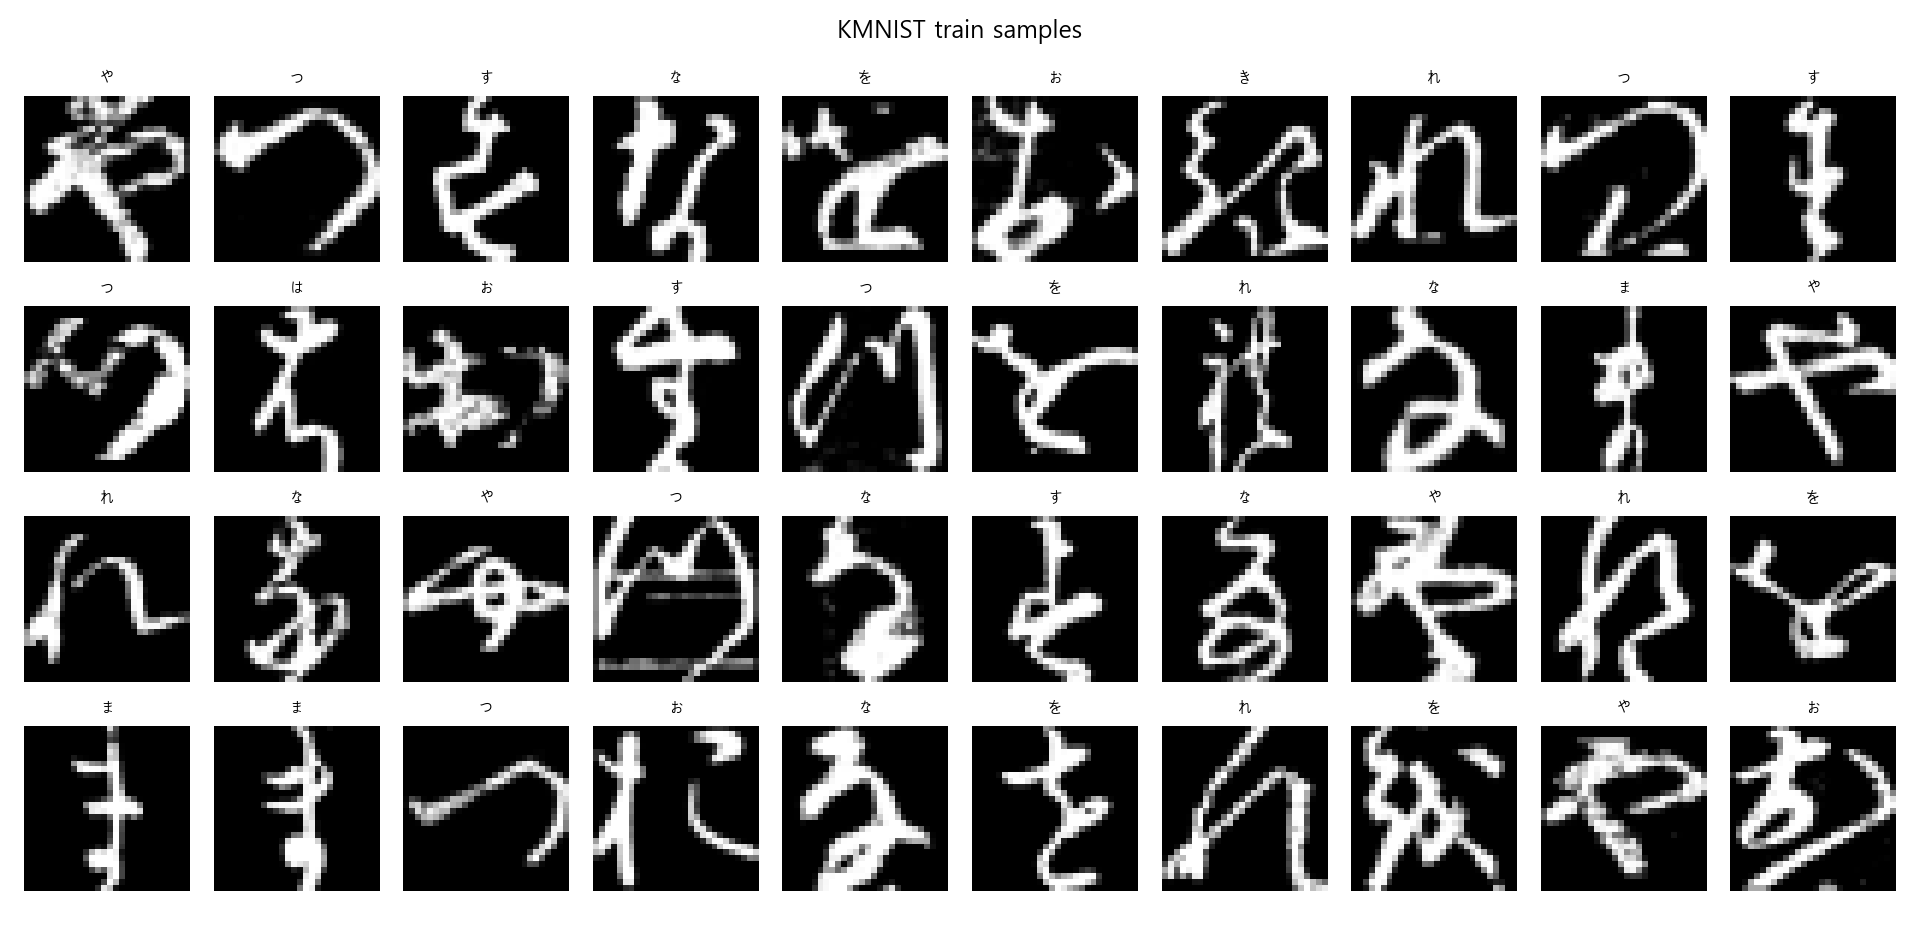
\includegraphics[width=\linewidth]{kmnist_train_samples.png}
        \caption{KMNIST train samples}
    \end{subfigure}
    \begin{subfigure}{0.48\linewidth}
        \centering
        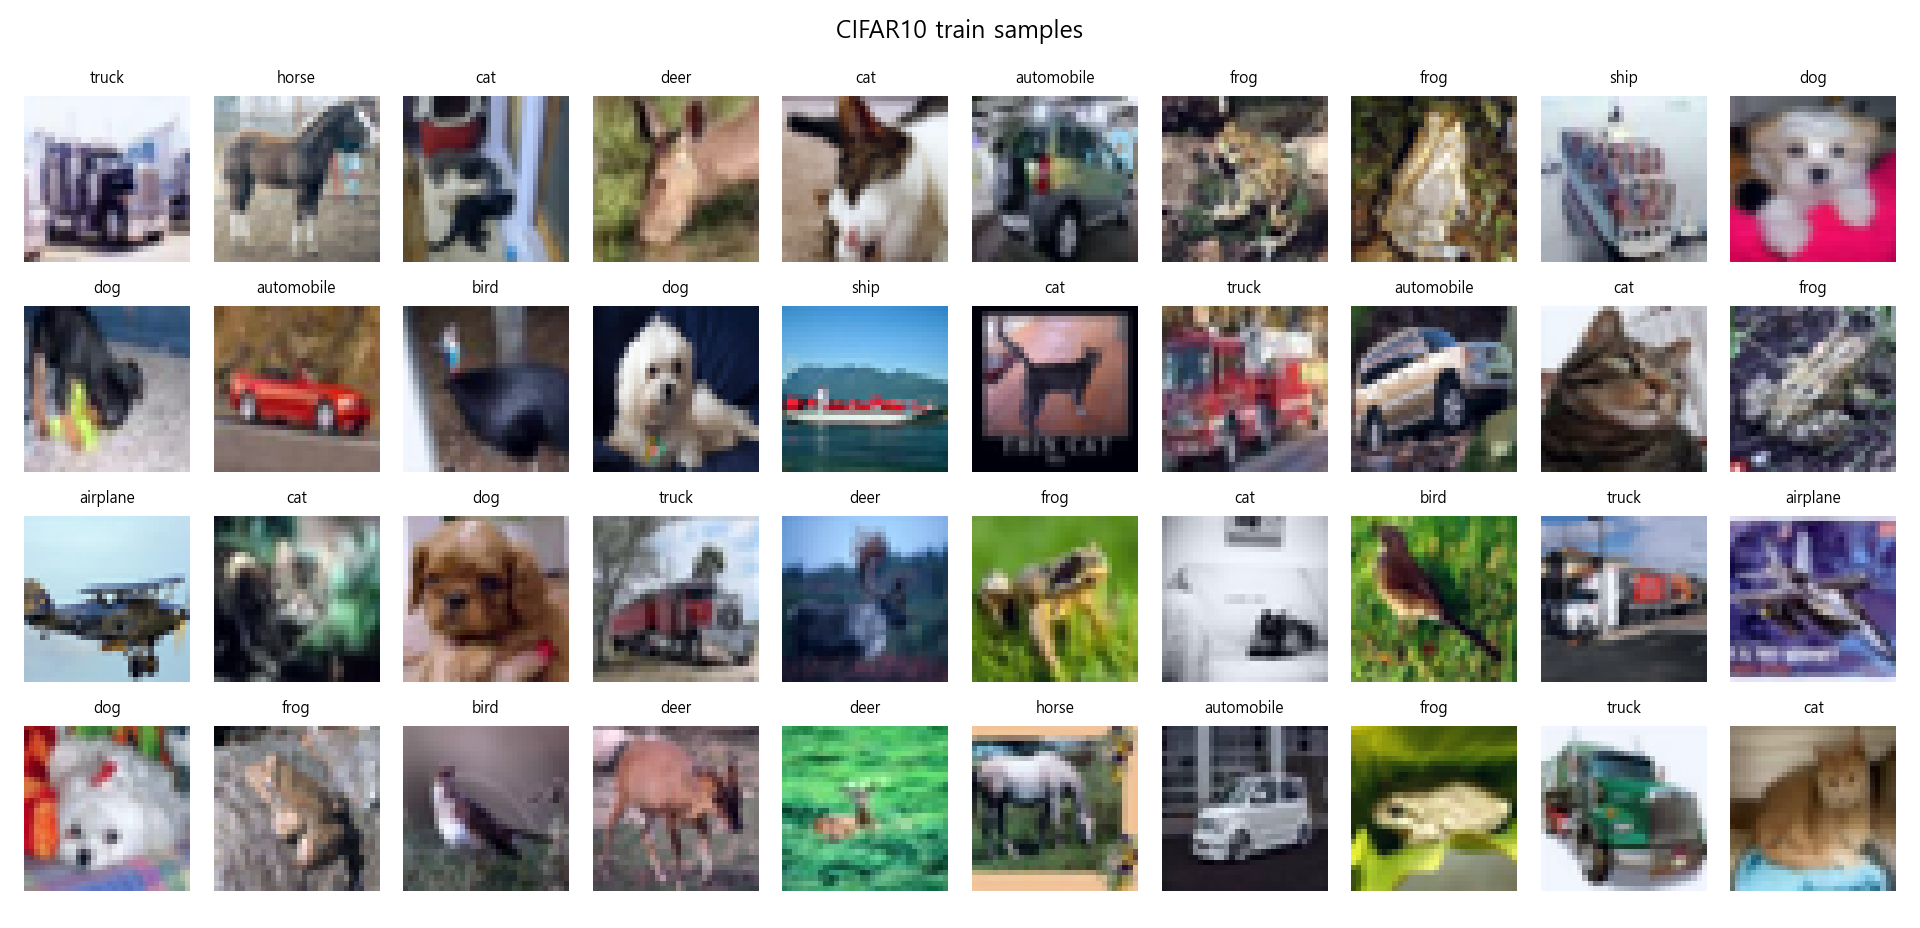
\includegraphics[width=\linewidth]{cifar10_train_samples.png}
        \caption{CIFAR-10 train samples}
    \end{subfigure}
    \caption{Dataset examples. KMNIST consists of simple grayscale handwritten characters, while CIFAR-10 contains RGB natural images with larger intra-class variation.}
    \label{fig:dataset-samples}
\end{figure}

\subsection{Feature Representations}

Required component 로 세 가지 feature representation 을 비교하였다.

\begin{itemize}[leftmargin=*]
    \item \textbf{PCA feature}: 이미지를 flatten 한 뒤 PCA 로 차원을 줄였다. 대표 비교에는 KMNIST 10차원, CIFAR-10 100차원을 포함하였고, component sweep 을 추가로 수행하여 차원 선택의 영향을 확인하였다.
    \item \textbf{AutoEncoder feature}: AutoEncoder 를 reconstruction loss 로 학습한 뒤 encoder output 을 사용하였다. 대표 비교에는 KMNIST MLP AutoEncoder 의 256차원 latent feature 와 CIFAR-10 convolutional AutoEncoder 의 64차원 latent feature 를 포함하였고, latent dimension 과 epoch sweep 을 추가로 수행하였다.
    \item \textbf{CNN feature}: CNN classifier 를 먼저 학습하고, classifier 직전 embedding 을 clustering feature 로 사용하였다. SmallCNN 과 ResNet18 을 비교하였다.
\end{itemize}

PCA 와 AutoEncoder 의 feature dimension 은 임의로 하나만 정하지 않고, 여러 후보를 비교하였다.
PCA component sweep 은 두 데이터셋 모두 같은 후보 \(\{2,10,20,50,100,200,300\}\)로 맞추었다.
AutoEncoder latent dimension sweep 도 두 데이터셋 모두 같은 후보 \(\{4,8,16,32,64,128,256,512\}\)로 맞추었다.

\begin{figure}[H]
    \centering
    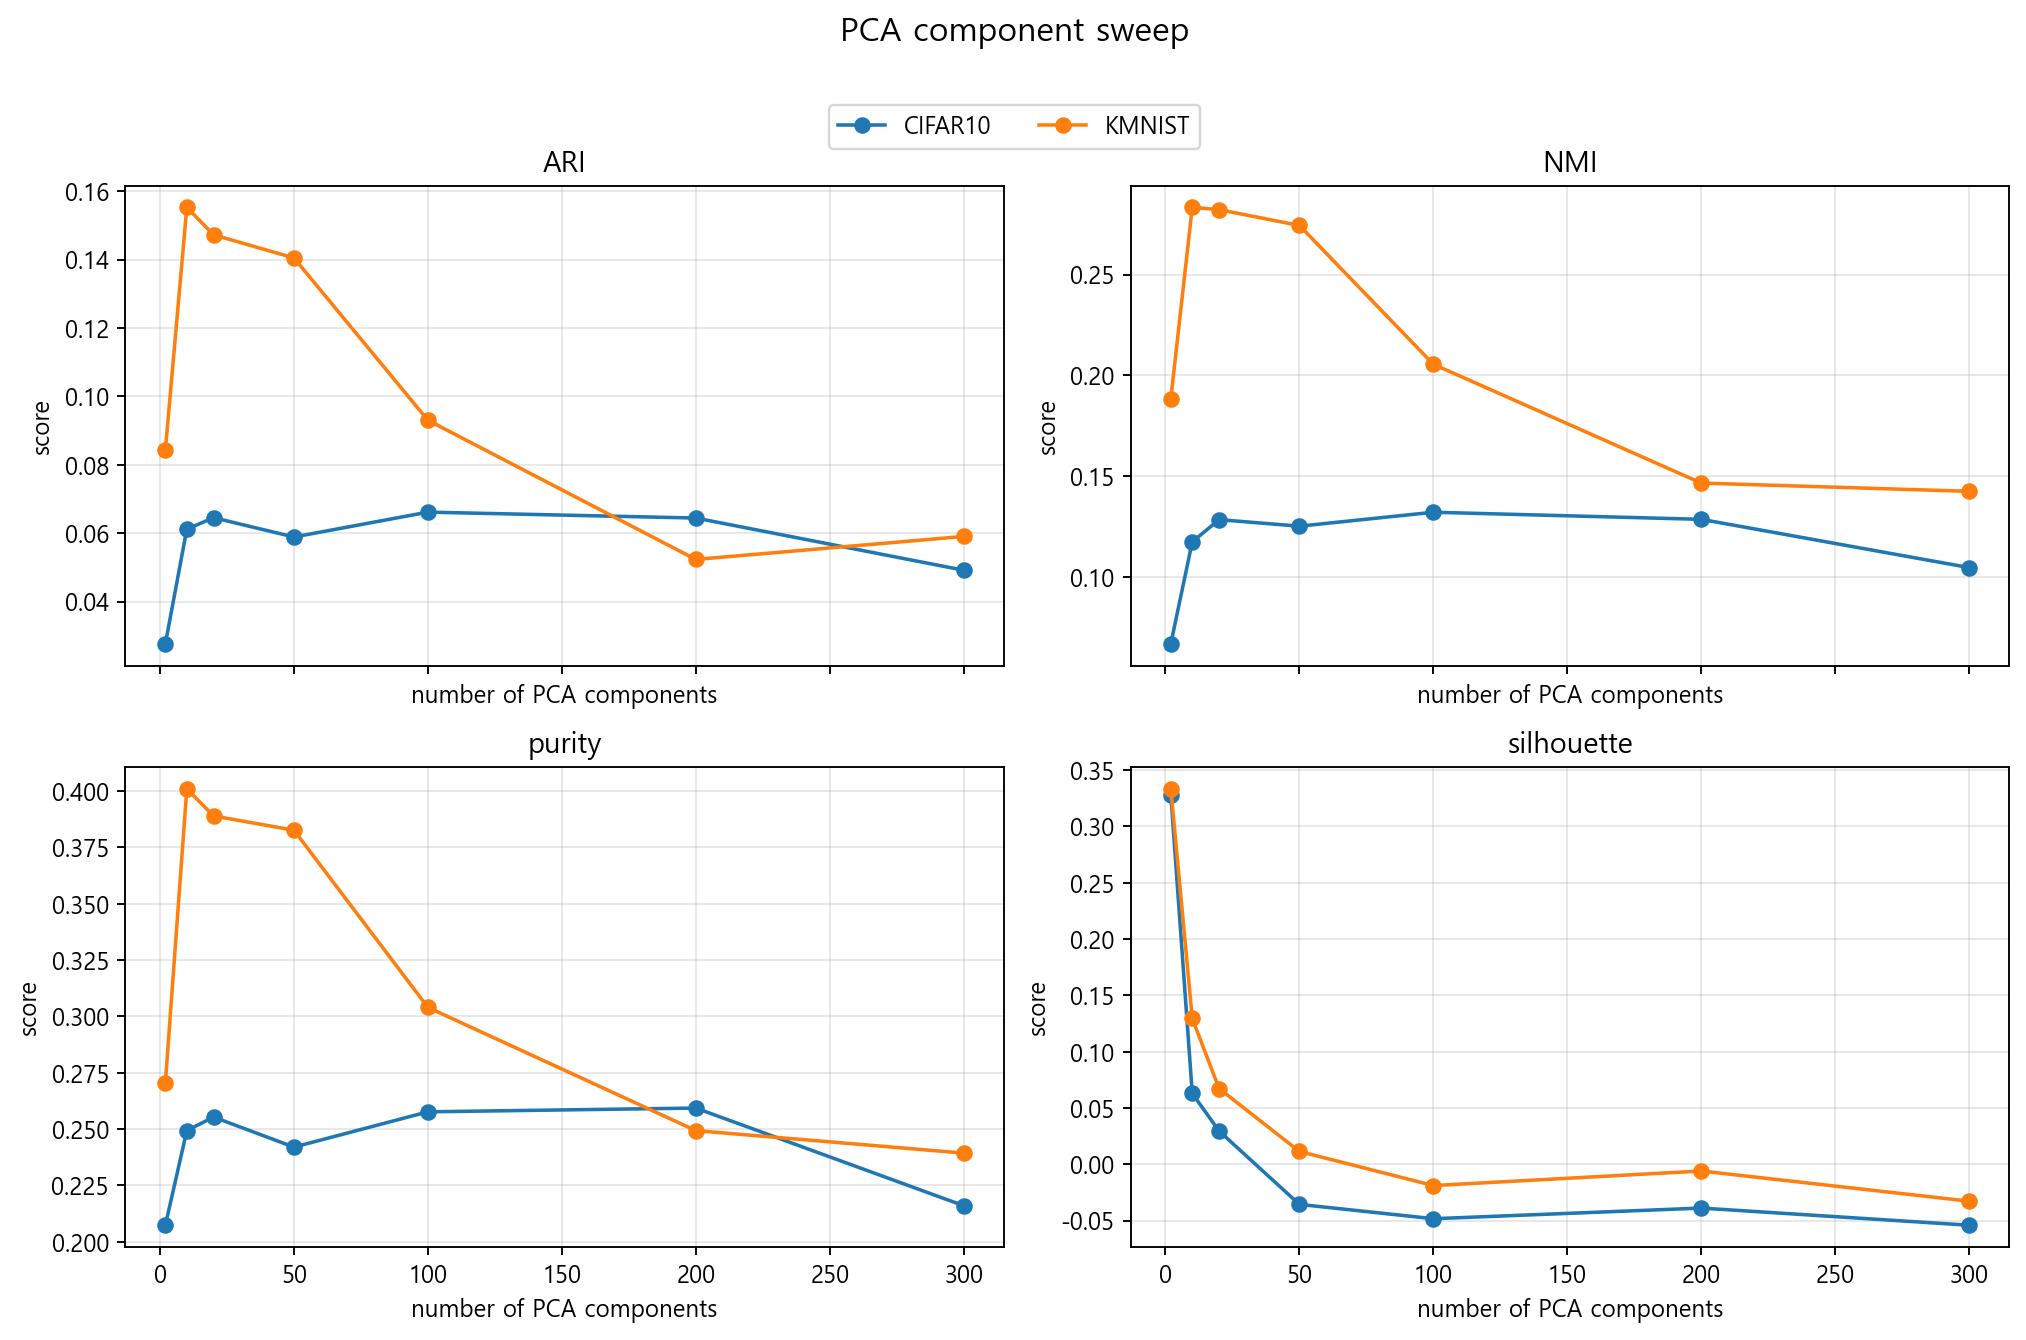
\includegraphics[width=\linewidth]{pca_component_sweep_metrics.png}
    \caption{Clustering metrics for different PCA dimensions.}
    \label{fig:pca-component-sweep}
\end{figure}

\begin{figure}[H]
    \centering
    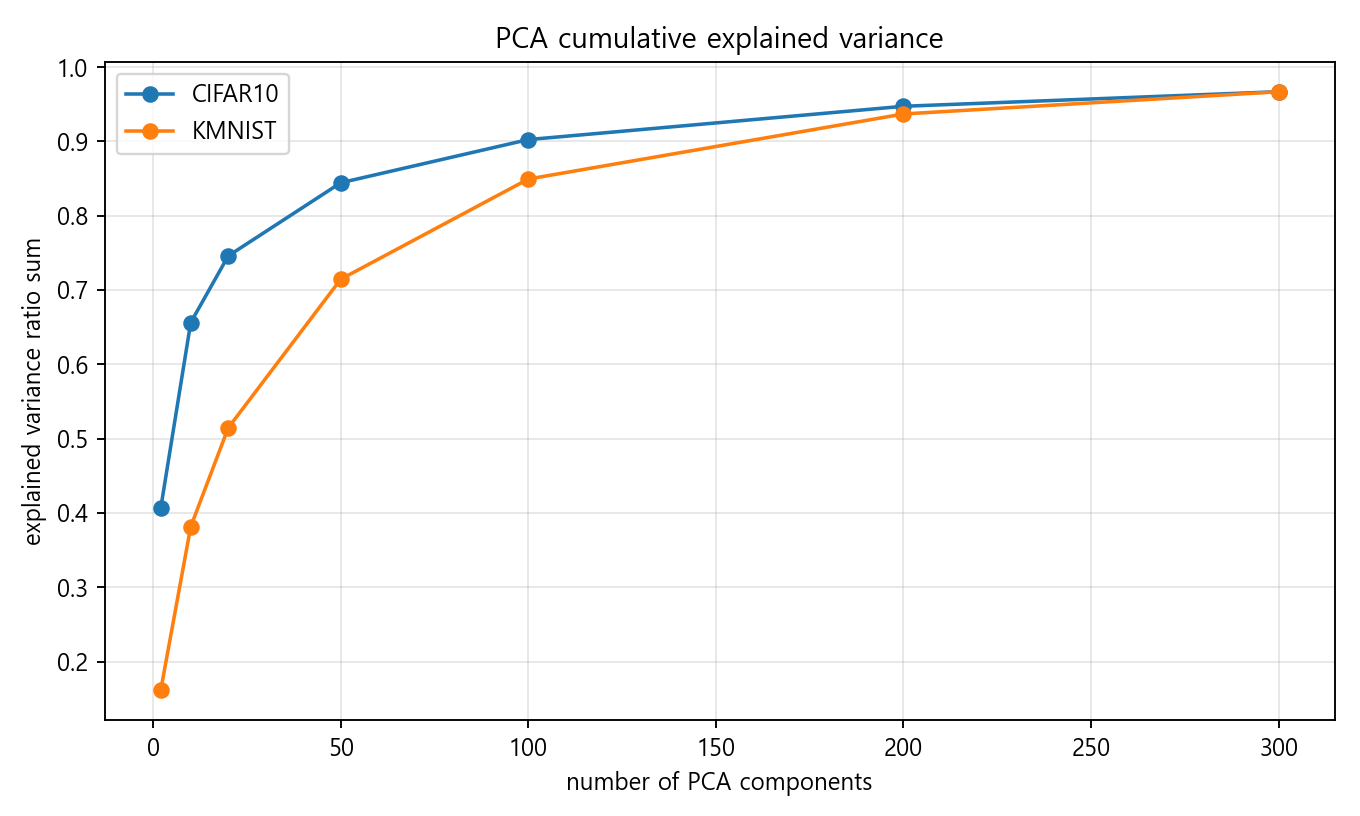
\includegraphics[width=0.78\linewidth]{pca_component_sweep_explained_variance.png}
    \caption{Cumulative explained variance for different PCA dimensions.}
    \label{fig:pca-explained-variance}
\end{figure}

Figure~\ref{fig:pca-component-sweep}와 Figure~\ref{fig:pca-explained-variance}를 같이 보면, PCA 의 explained variance 와 clustering metric 이 같은 방향으로 움직이지 않는다.
KMNIST 는 10 components 에서 ARI 0.1553으로 가장 높았지만, explained variance 는 300 components 에서 0.9667까지 계속 증가하였다.
CIFAR-10 은 100 components 에서 ARI 0.0662로 가장 높았고, 200 components 와 300 components 에서는 더 많은 variance 를 보존해도 ARI 가 개선되지 않았다.
따라서 PCA feature dimension 은 분산 보존량만 보고 정하기보다, clustering metric 을 함께 확인해야 한다.

\begin{figure}[H]
    \centering
    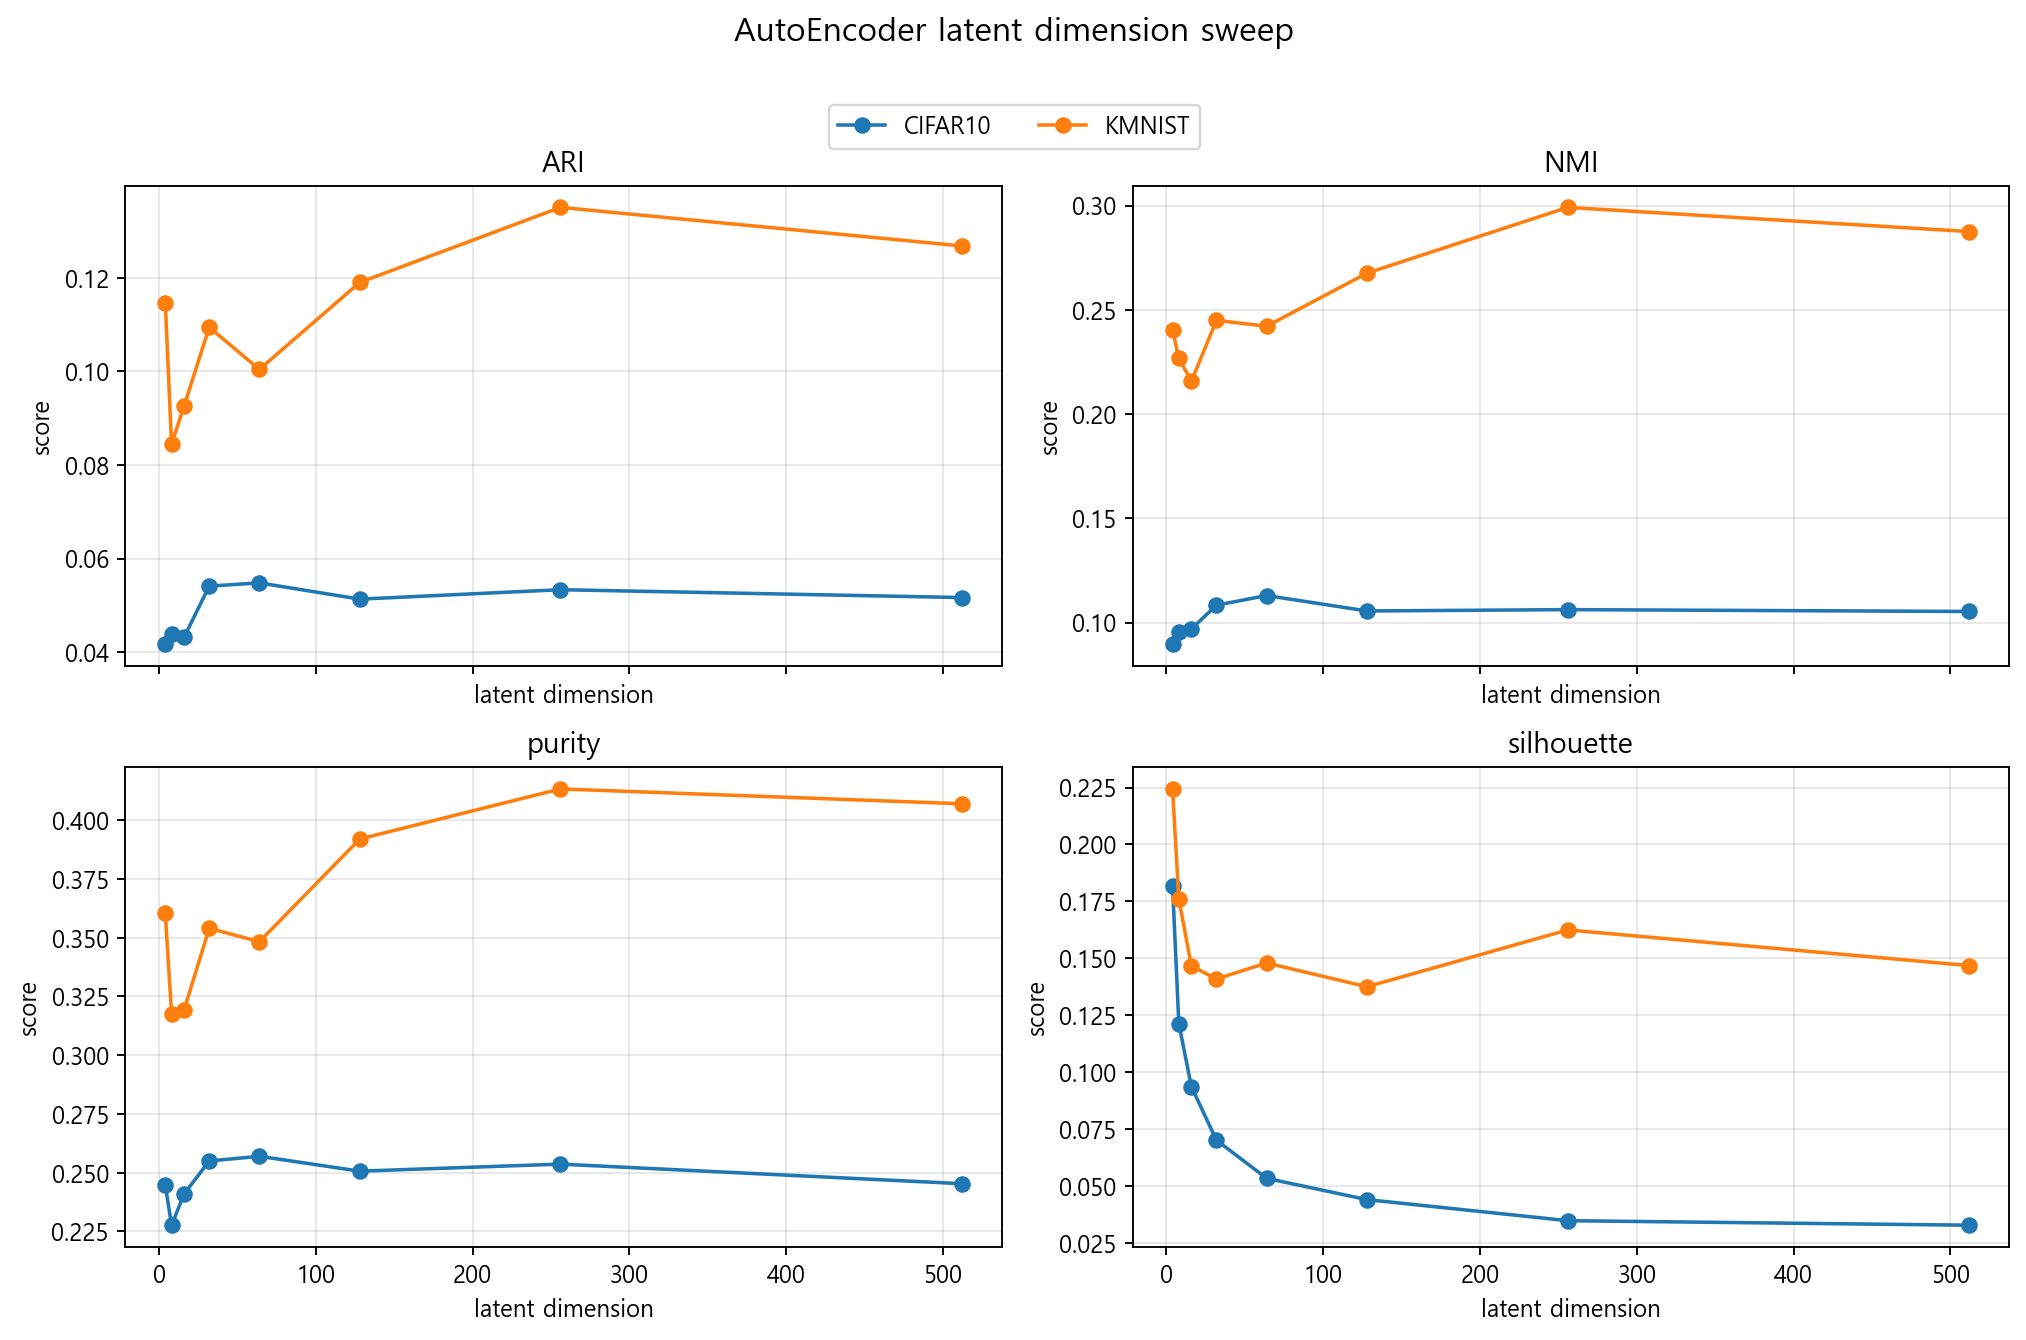
\includegraphics[width=\linewidth]{ae_latent_dim_sweep_metrics.png}
    \caption{Clustering metrics for different AutoEncoder latent dimensions.}
    \label{fig:ae-latent-sweep}
\end{figure}

\begin{figure}[H]
    \centering
    \begin{subfigure}{0.49\linewidth}
        \centering
        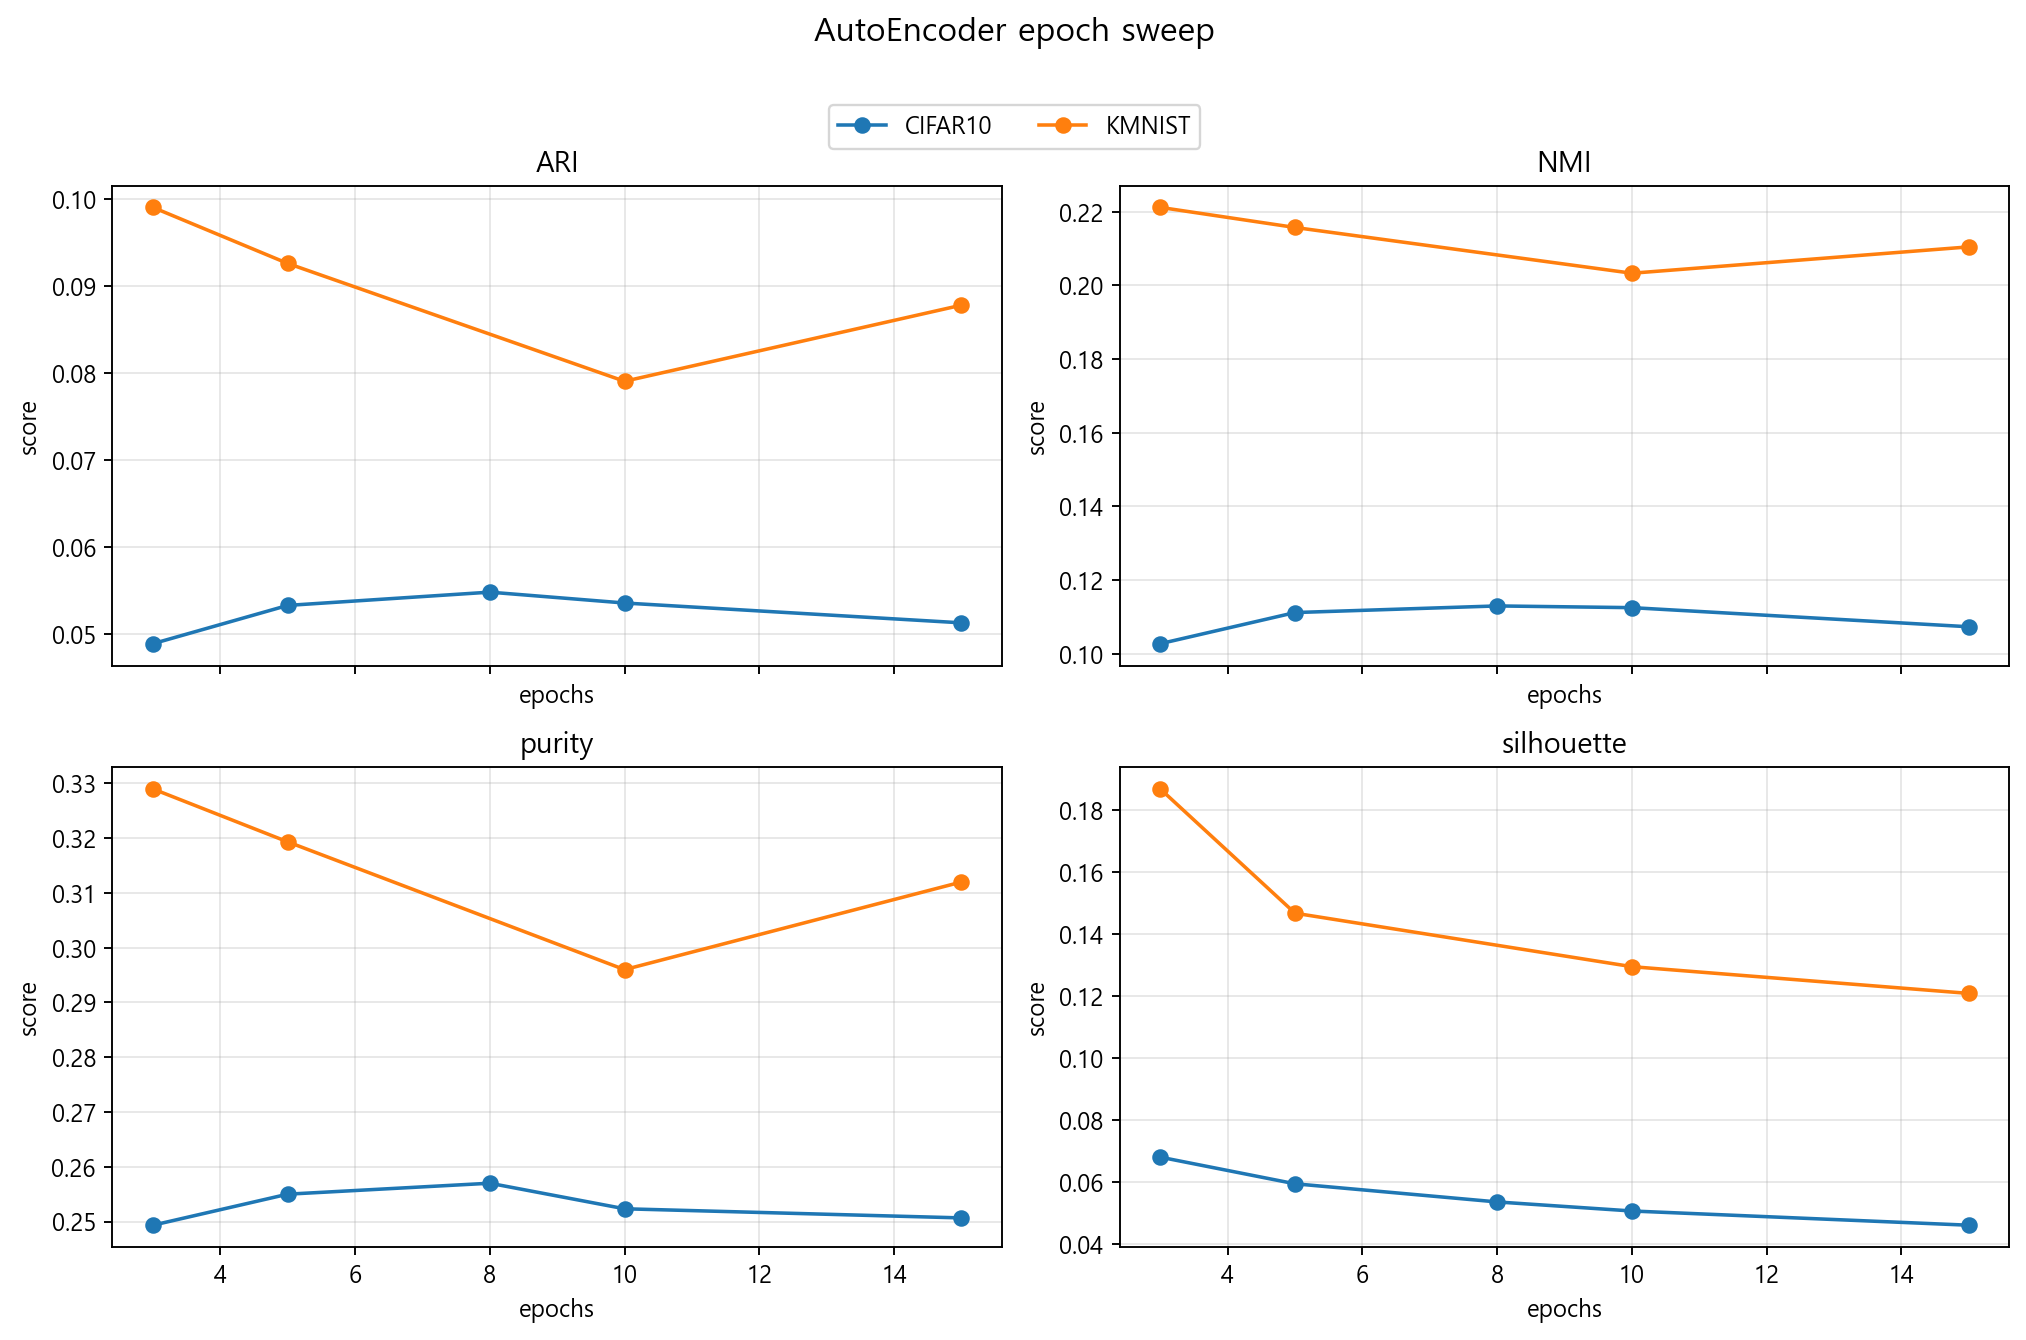
\includegraphics[width=\linewidth]{ae_epoch_sweep_metrics.png}
        \caption{Clustering metrics}
    \end{subfigure}
    \begin{subfigure}{0.49\linewidth}
        \centering
        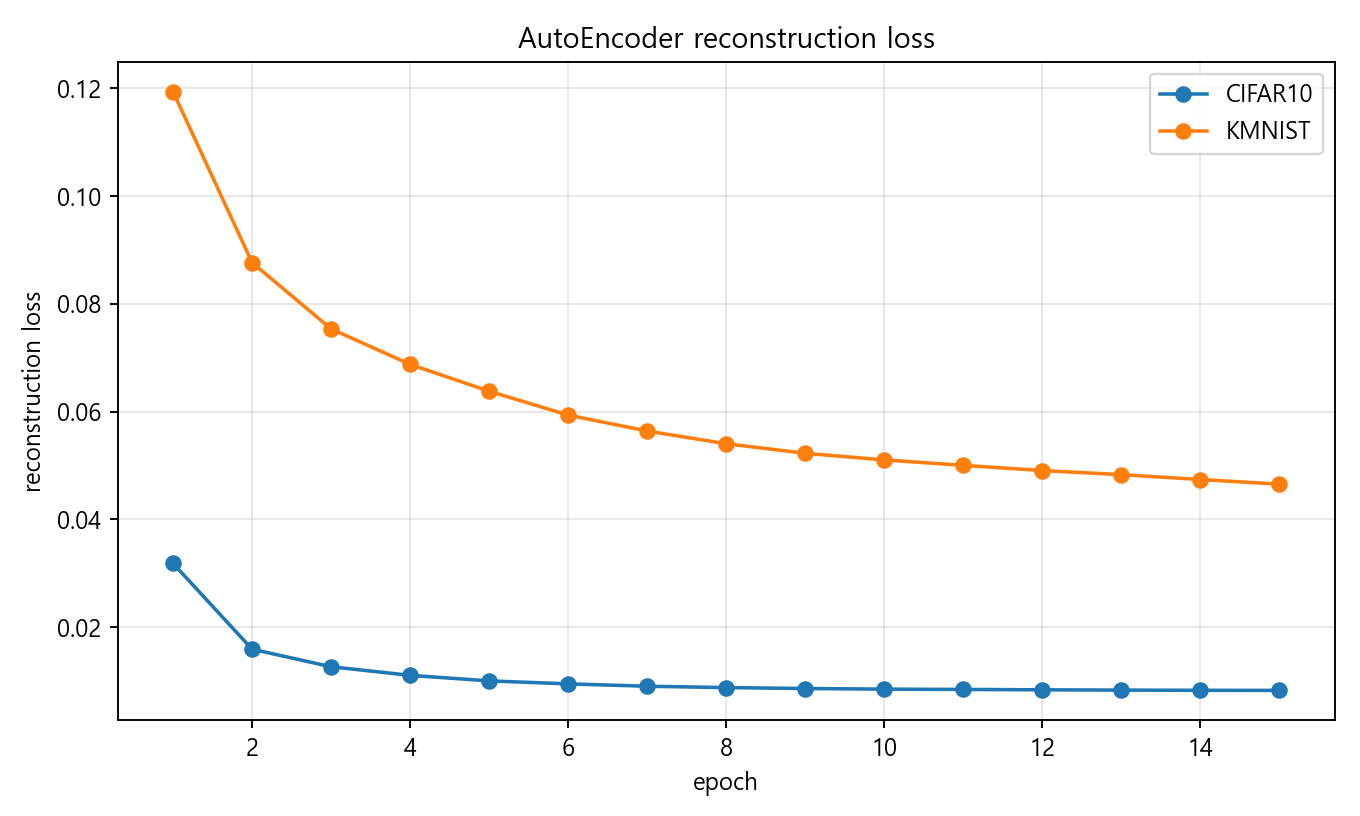
\includegraphics[width=\linewidth]{ae_reconstruction_loss_curves.png}
        \caption{Reconstruction loss}
    \end{subfigure}
    \caption{AutoEncoder epoch sweep at fixed latent dimensions. Reconstruction loss decreases with training, but clustering metrics do not improve in the same direction.}
    \label{fig:ae-epoch-sweep}
\end{figure}

Figure~\ref{fig:ae-latent-sweep}에서는 CIFAR-10 ConvAE 가 latent dimension 32--64 근처에서 plateau 를 보인다.
64차원에서 ARI 0.0548로 가장 높고, 128, 256, 512로 늘려도 개선되지 않았다.
KMNIST MLP AutoEncoder 는 256차원에서 ARI 0.1351로 가장 높았지만, 512차원에서는 0.1268로 낮아졌다.
즉 AutoEncoder latent dimension 을 키우는 것이 일정 구간에서는 도움이 될 수 있지만, CNN feature 와의 큰 성능 차이를 해결하지는 못했다.
Figure~\ref{fig:ae-epoch-sweep}에서도 reconstruction loss 는 계속 낮아지지만 clustering metric 은 함께 상승하지 않는다.
이는 AutoEncoder 가 image reconstruction 을 목표로 학습되며, class-separable latent space 를 직접 만들도록 강제되지 않기 때문이다.

SmallCNN 은 convolution block 을 쌓은 구조이며, 기본형은 channel \([32,64,128]\), embedding 128 차원이다.
두 데이터셋 모두에서 더 큰 비교군으로 channel \([64,128,256]\), embedding 256 차원의 wider SmallCNN 도 실험하였다.
다만 dataset 특성에 맞추어 augmentation 은 다르게 적용하였다.
Table~\ref{tab:cnn-settings}는 CNN 비교군의 주요 설정이다.

\begin{table}[H]
    \centering
    \caption{CNN feature extractor settings.}
    \label{tab:cnn-settings}
    \begin{tabular}{llcccc}
        \toprule
        Dataset & Model & Channels & Embedding & Augmentation & Epochs\\
        \midrule
        KMNIST & SmallCNN & \([32,64,128]\) & 128 & none & 5\\
        KMNIST & Wider SmallCNN & \([64,128,256]\) & 256 & affine / translate & 12\\
        KMNIST & ResNet18 & residual blocks & 128 & affine / translate & 20\\
        CIFAR-10 & Wider SmallCNN & \([64,128,256]\) & 256 & crop / flip & 20\\
        CIFAR-10 & ResNet18 & residual blocks & 128 & crop / flip & 20\\
        \bottomrule
    \end{tabular}
\end{table}

Lab2 example code 에서 나온 BatchNorm, Dropout 과 같은 추가 방법들의 흐름을 확장하여 실험을 세팅하였다.
Dropout 은 training 중 일부 embedding unit 을 확률적으로 0으로 만들어 특정 feature 에 과하게 의존하는 것을 줄이는 regularization 방법이다.
본 실험에서는 wider SmallCNN 에 dropout 0.25 를 적용하였다.
Random crop 은 CIFAR-10 image 주변을 padding 한 뒤 다시 \(32\times32\) 로 잘라내어 object 위치 변화에 덜 민감하게 만드는 augmentation 이다.
Horizontal flip 은 자연 이미지의 좌우 반전이 대체로 class 의미를 바꾸지 않는다는 점을 이용한 augmentation 이다.
반면 KMNIST 에서는 좌우 반전이 문자 모양 자체를 바꿀 수 있으므로 horizontal flip 은 사용하지 않았고, 작은 회전과 이동을 주는 random affine / translation 만 사용하였다.

ResNet18 은 CIFAR-size image 에 맞게 첫 convolution 을 \(3\times3\), stride 1 로 두고 초기 max-pooling 을 사용하지 않는 형태로 구현하였다.
Embedding dimension 은 128 로 고정하였다.
ResNet18 optimizer 는 SGD, learning rate 0.05, momentum 0.9, weight decay \(5\times10^{-4}\)를 사용하였고, 20 epochs 학습하였다.

\subsection{Clustering Methods}

Clustering 은 feature 를 StandardScaler 로 scaling 한 뒤 수행하였다.
K-means 는 cluster 수를 class 수와 같은 10으로 두었고, \texttt{n\_init=50}, \texttt{max\_iter=500}을 사용하였다.
GMM 도 component 수를 10으로 두었고, \texttt{covariance\_type=diag}, \texttt{n\_init=3}, \texttt{reg\_covar=1e-4}를 사용하였다.
GMM covariance estimation 은 numerical stability 를 위해 float64 feature 로 수행하였다.

\subsection{Evaluation Metrics}

본 보고서에서는 ARI, NMI, purity, silhouette 를 사용하였다.
여기서 \(U\)는 clustering 결과, \(V\)는 true class label, \(N\)은 sample 수를 의미한다.

\begin{itemize}[leftmargin=*]
    \item \textbf{ARI}: true label pair 와 cluster pair 의 일치도를 chance correction 한 값이다. Label permutation 에 영향을 받지 않아 clustering 평가에 적합하다.
    \[
        ARI =
        \frac{
        \text{Index} - \text{Expected Index}
        }{
        \text{Max Index} - \text{Expected Index}
        }
    \]
    \item \textbf{NMI}: true label 과 cluster label 사이의 mutual information 을 entropy 로 normalize 한 값이다. Cluster 가 class 정보를 얼마나 보존하는지 본다.
    \[
        MI(U,V) =
        \sum_i \sum_j
        P(U_i, V_j)
        \log
        \frac{
        P(U_i, V_j)
        }{
        P(U_i)P(V_j)
        }
    \]
    \[
        NMI(U,V) =
        \frac{
        MI(U,V)
        }{
        \sqrt{H(U)H(V)}
        }
    \]
    \item \textbf{Purity}: 각 cluster 에서 가장 많은 true class 를 맞았다고 보고 계산한 비율이다. 직관적이지만 chance correction 은 없다.
    \[
        \mathrm{Purity}(U,V) =
        \frac{1}{N}
        \sum_i \max_j |U_i \cap V_j|
    \]
    \item \textbf{Silhouette}: feature space 에서 같은 cluster 내부 거리는 작고, 다른 cluster 와의 거리는 큰지 보는 geometric metric 이다.
    \[
        a(i) = \text{same-cluster mean distance}, \qquad
        b(i) = \text{nearest other-cluster mean distance}
    \]
    \[
        s(i) =
        \frac{
        b(i) - a(i)
        }{
        \max(a(i), b(i))
        }
    \]
\end{itemize}

시각화는 dataset sample grid, PCA/t-SNE 2D embedding, cluster-class heatmap, cluster별 sample grid, wrong mapping example grid 를 사용하였다.

\section{Results on KMNIST}

\subsection{Quantitative Results}

Table~\ref{tab:kmnist-results}는 KMNIST test set 결과이다.
PCA 와 AutoEncoder feature 는 낮은 ARI/NMI 를 보였고, CNN feature 부터 class structure 가 뚜렷하게 나타났다.
KMNIST 에서는 feature extractor 의 성격이 clustering 결과를 거의 결정하였다.
같은 K-means 를 사용하더라도 PCA10 은 ARI 0.1553, AE256 은 ARI 0.1351 에 머물렀지만, SmallCNN128 은 ARI 0.6492 까지 상승하였다.
ResNet18 을 사용하면 12k subset 에서도 ARI 0.8916 을 얻었고, full train split 에서는 ARI 0.9284 까지 개선되었다.

\begin{table}[H]
    \centering
    \caption{KMNIST test results.}
    \label{tab:kmnist-results}
    \small
    \begin{tabular}{lccccc}
        \toprule
        Feature / clustering & Train size & ARI & NMI & Purity & Silhouette\\
        \midrule
        PCA10 + K-means & 12k & 0.1553 & 0.2834 & 0.4010 & 0.1295\\
        AE256 + K-means & 12k & 0.1351 & 0.2992 & 0.4133 & 0.1625\\
        SmallCNN128 + K-means & 12k & 0.6492 & 0.7100 & 0.8147 & 0.2374\\
        SmallCNN256 + K-means & 12k & 0.5886 & 0.7225 & 0.7793 & 0.1923\\
        ResNet18 + K-means & 12k & 0.8916 & 0.8957 & 0.9493 & 0.4500\\
        ResNet18 + GMM & 12k & 0.8611 & 0.8675 & 0.9350 & 0.4412\\
        SmallCNN128 + K-means & full & 0.8186 & 0.8276 & 0.9139 & 0.2451\\
        \textbf{ResNet18 + K-means} & \textbf{full} & \textbf{0.9284} & \textbf{0.9238} & \textbf{0.9672} & \textbf{0.5426}\\
        ResNet18 + GMM & full & 0.7023 & 0.8279 & 0.8782 & 0.4594\\
        \bottomrule
    \end{tabular}
\end{table}

\subsubsection{PCA and AutoEncoder Features}

PCA10 + K-means 는 PCA 기반 대표 baseline 이다.
이미지를 flatten 한 뒤 분산이 큰 방향을 보존하므로 stroke 의 굵기, 위치, 전체적인 pixel 변화는 반영하지만, class label 을 직접 분리하도록 학습되지는 않는다.
그 결과 test ARI 는 0.1553, purity 는 0.4010 으로 낮았다.
Figure~\ref{fig:kmnist-all-tsne}의 PCA panel 에서도 cluster 색이 중심부에서 많이 섞이고, Figure~\ref{fig:kmnist-all-heatmaps}에서도 한 cluster 행이 여러 true class 열로 퍼져 있다.

\begin{figure}[H]
    \centering
    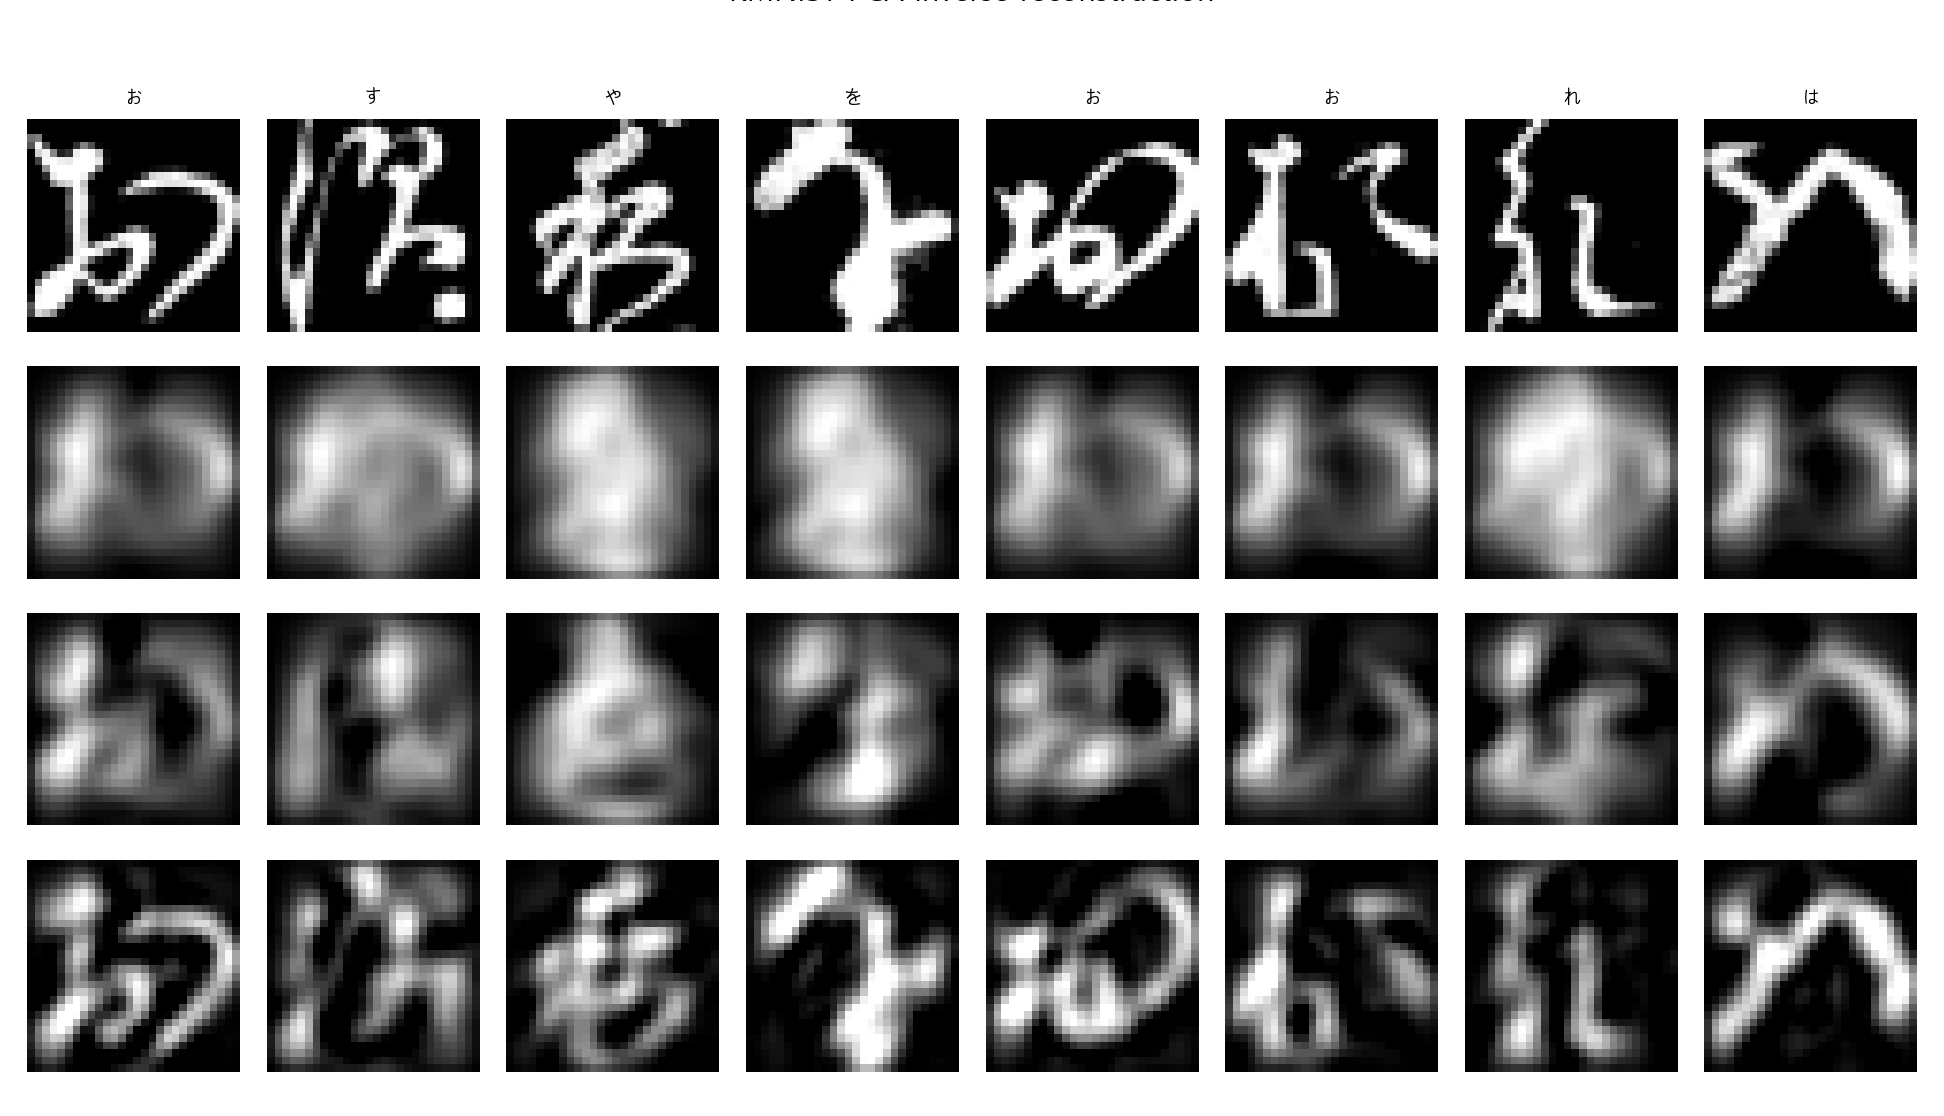
\includegraphics[width=0.92\linewidth]{kmnist_pca10_kmeans_pca_reconstruction.png}
    \caption{KMNIST PCA inverse reconstruction examples. Increasing the number of components restores more stroke structure, but low-dimensional PCA reconstructions remain blurry and lose fine local details.}
    \label{fig:kmnist-pca-reconstruction}
\end{figure}

Figure~\ref{fig:kmnist-pca-reconstruction}은 PCA feature 를 다시 원래 image space 로 inverse transform 한 결과이다.
Component 수가 작을 때는 문자 윤곽만 흐릿하게 남고, 대표 설정인 10 components 에서도 얇은 획과 국소적인 stroke 차이는 완전히 복원되지 않는다.
이는 PCA feature 가 pixel-level variance 는 보존하지만, 문자 class 를 구분하는 세밀한 획 구조를 충분히 안정적으로 보존하지 못했음을 보여준다.

AE256 + K-means 는 ARI 0.1351 을 보였다.
Silhouette 은 0.1625 로 PCA10 의 0.1295 보다 조금 높았다.
이는 AutoEncoder latent space 에서 어떤 geometric cluster 는 만들어졌지만, 그 cluster 가 실제 character class 와 잘 맞지는 않았다는 의미이다.
AutoEncoder 는 reconstruction loss 를 줄이도록 학습되므로, class 구분보다 stroke 복원에 필요한 굵기, 위치, local pattern 을 보존하는 쪽으로 latent feature 가 형성될 수 있다.

\begin{figure}[H]
    \centering
    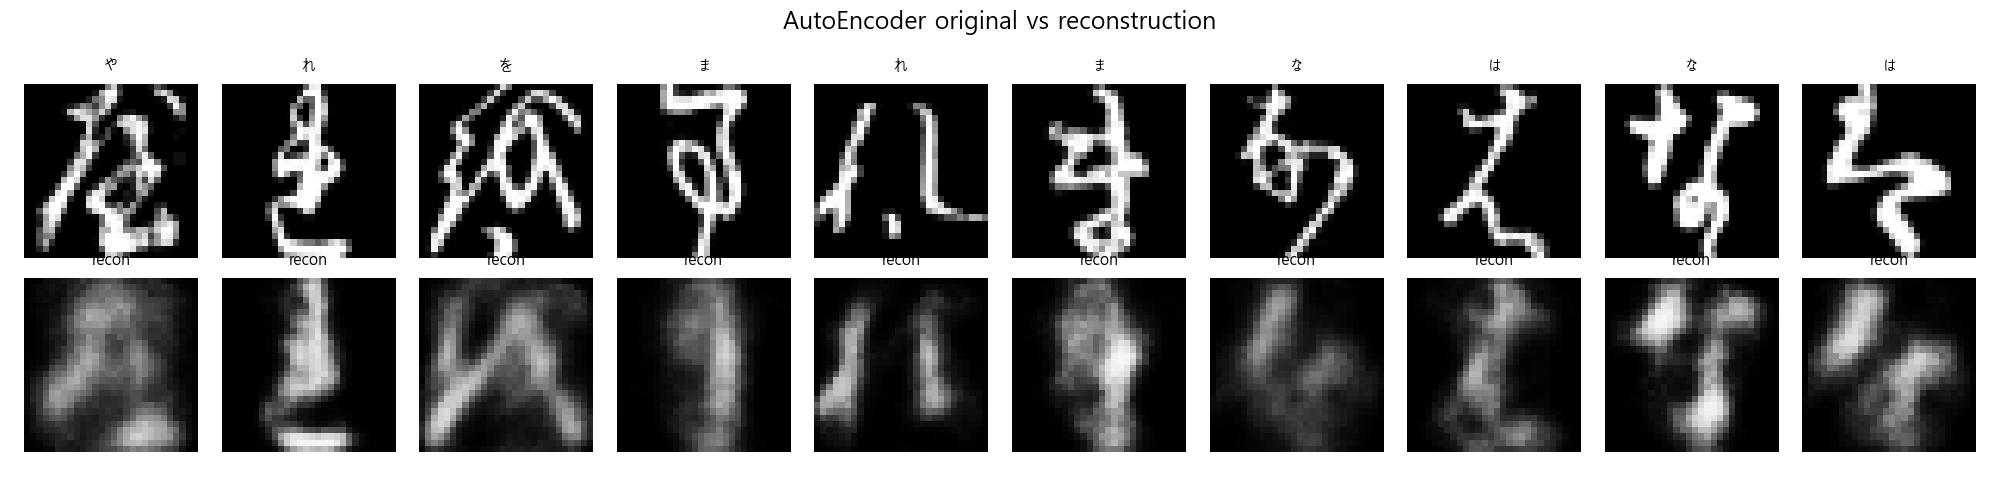
\includegraphics[width=0.80\linewidth]{kmnist_ae256_e5_kmeans_reconstruction_grid.png}
    \caption{KMNIST AutoEncoder reconstruction examples. The reconstructed images preserve rough stroke shapes, but this does not directly imply class-separable latent features.}
    \label{fig:kmnist-ae-reconstruction}
\end{figure}

Figure~\ref{fig:kmnist-ae-reconstruction}에서 복원 이미지는 원본의 대략적인 획 방향과 전체 윤곽은 유지하지만, 세부 stroke 가 흐릿하고 얇은 획이 사라지는 경우가 보인다.
이는 AE256 latent 에도 reconstruction 에 필요한 coarse shape 정보와 class 구분에 필요한 fine-grained stroke 정보가 완전히 같지는 않다는 점을 보여준다.

\subsubsection{SmallCNN Features}

SmallCNN128 + K-means 부터 결과가 크게 달라졌다.
Test ARI 는 0.6492, NMI 는 0.7100, purity 는 0.8147 이었다.
Supervised classifier 로 학습한 CNN embedding 은 label prediction 에 필요한 정보를 담기 때문에, PCA/AE feature 보다 class-discriminative 하다.
다만 train ARI 는 0.9027 이었던 반면 test ARI 는 0.6492 로 내려가, 12k subset 과 작은 CNN 구조만으로는 test feature space 가 완전히 안정적이지 않았다.

SmallCNN256 + K-means 는 channel 을 \([64,128,256]\)으로 늘리고 embedding 을 256차원으로 키운 설정이다.
NMI 는 0.7225 로 SmallCNN128 보다 약간 높았지만, ARI 는 0.5886, purity 는 0.7793 으로 낮아졌다.
즉 더 큰 CNN 이 class 정보량을 조금 더 담았을 수는 있지만, K-means 가 보기 좋은 10개의 균형 잡힌 cluster 로 정리되지는 않았다.
Figure~\ref{fig:kmnist-all-tsne}에서도 SmallCNN256 은 여러 작은 island 가 생기지만 일부 cluster 가 쪼개지거나 가까운 영역에서 섞이는 모습이 남아 있다.
따라서 KMNIST 에서는 단순히 channel 수와 embedding dimension 을 키우는 것만으로는 clustering 성능이 보장되지 않았다.

SmallCNN128 을 full train split 으로 학습한 경우 ARI 는 0.8186 까지 상승하였다.
이는 KMNIST 에서 train set 크기도 중요한 요인임을 보여준다.
하지만 같은 full split 에서 ResNet18 + K-means 는 ARI 0.9284 를 얻었으므로, 단순히 sample 수만 늘리는 것보다 feature extractor 구조를 강화하는 효과가 더 컸다.

\subsubsection{ResNet18 Features}

ResNet18 + K-means 는 KMNIST 에서 가장 강한 조합이었다.
12k subset 만 사용해도 ARI 0.8916, purity 0.9493 을 얻었고, full train split 에서는 ARI 0.9284, purity 0.9672 로 더 좋아졌다.
Residual block 을 가진 ResNet18 은 stroke 의 작은 변형을 더 안정적으로 처리하며, classifier 직전 embedding 에서 class별 cluster 가 더 compact 하게 형성되었다.

\begin{figure}[H]
    \centering
    \begin{subfigure}{0.92\linewidth}
        \centering
        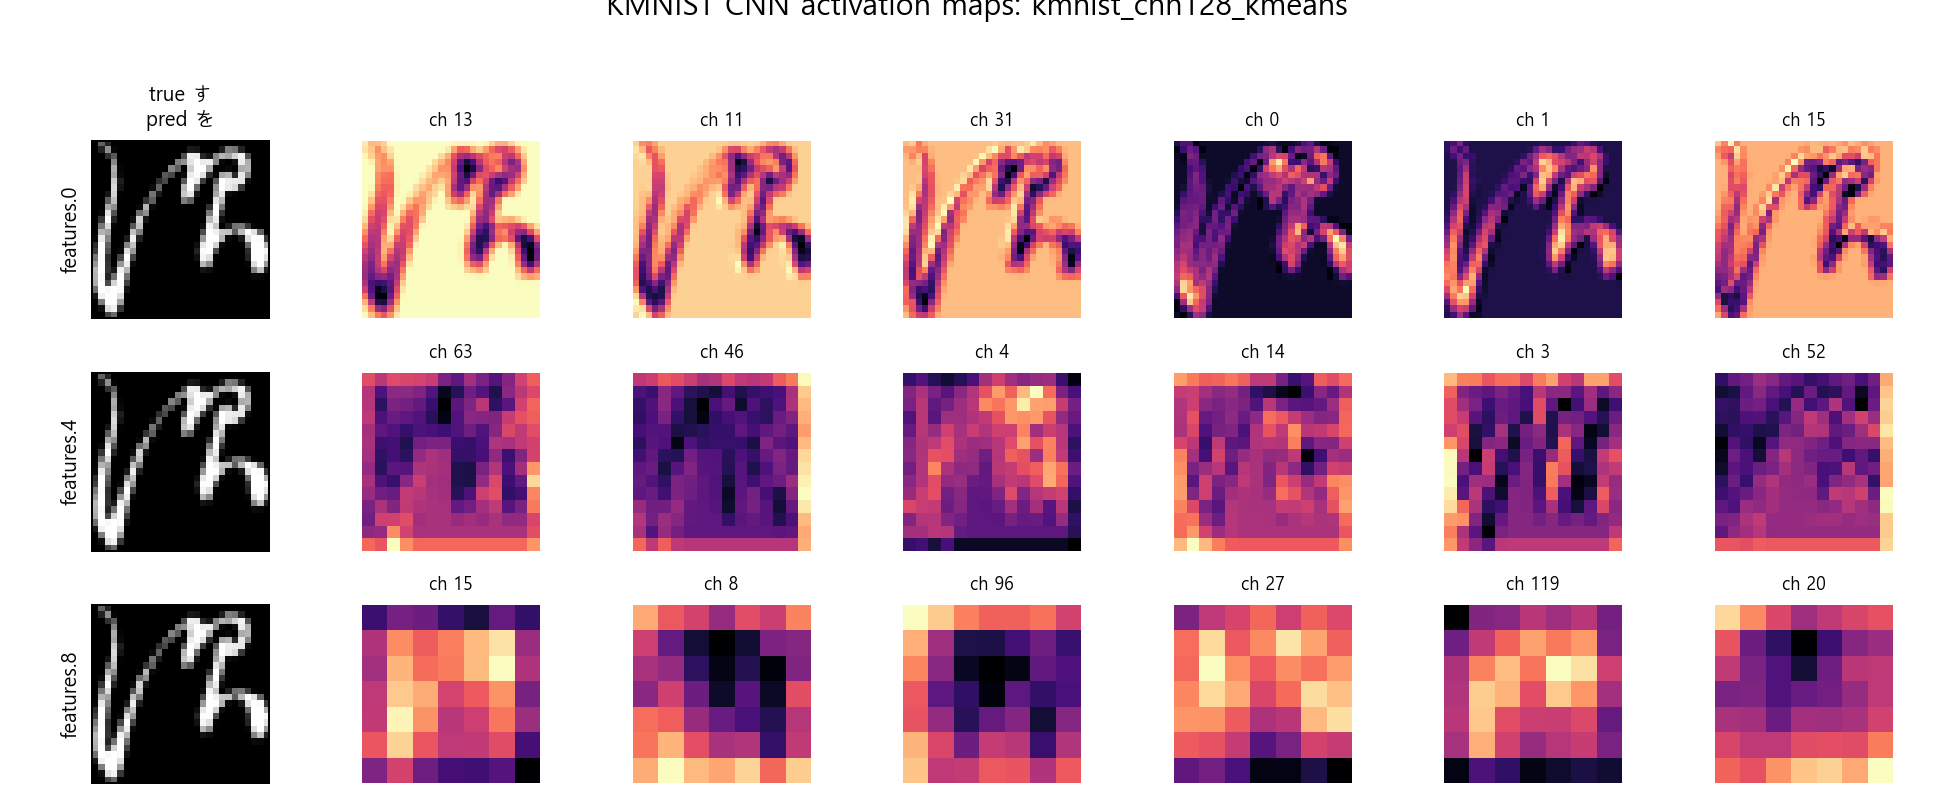
\includegraphics[width=\linewidth]{kmnist_cnn128_kmeans_activation_maps.png}
        \caption{SmallCNN128}
    \end{subfigure}
    \vspace{0.08in}
    \begin{subfigure}{0.92\linewidth}
        \centering
        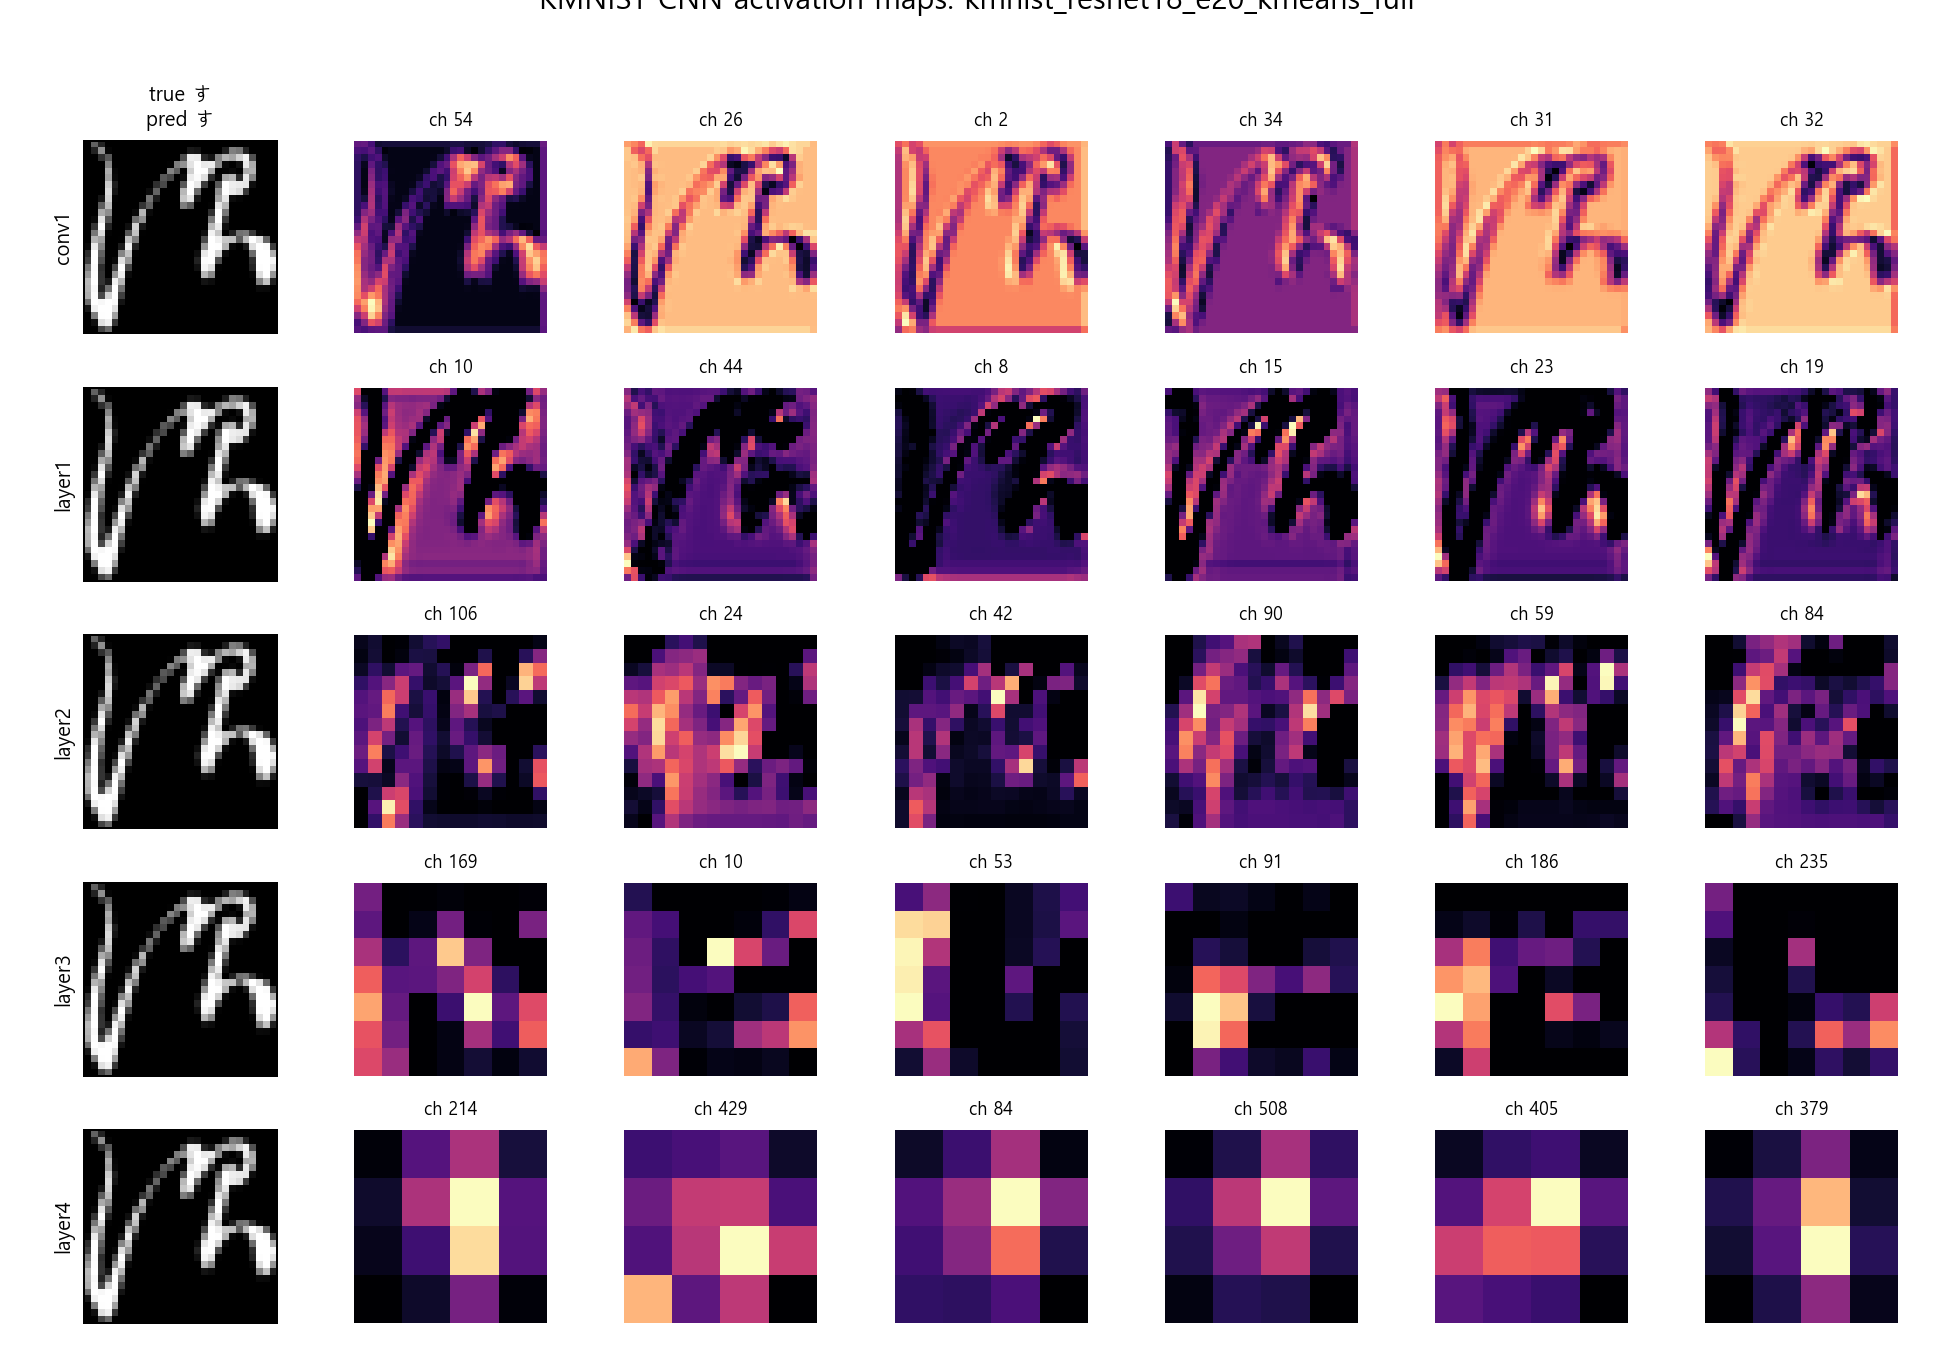
\includegraphics[width=\linewidth]{kmnist_resnet18_e20_kmeans_full_activation_maps.png}
        \caption{ResNet18}
    \end{subfigure}
    \caption{KMNIST CNN activation maps for the same raw test image. The true class is \jp{す}; SmallCNN predicts \jp{を}, while ResNet18 predicts \jp{す}.}
    \label{fig:kmnist-cnn-activation}
\end{figure}

Figure~\ref{fig:kmnist-cnn-activation}은 같은 raw test image 를 SmallCNN 과 ResNet18 에 넣고, CNN 내부 layer 의 activation map 을 forward hook 으로 저장한 것이다.
CNN classifier 는 AutoEncoder 와 달리 decoder 를 갖고 있지 않으므로 latent feature 를 이미지로 직접 복원할 수는 없다.
대신 activation map 을 보면 앞쪽 layer 는 획의 위치와 edge 에 강하게 반응하고, 뒤쪽 layer 로 갈수록 공간 해상도는 작아지지만 class 판단에 필요한 더 추상적인 pattern 으로 압축되는 것을 확인할 수 있다.
이 sample 의 실제 class 는 \jp{す}인데, SmallCNN 은 \jp{を}로 잘못 예측했고 ResNet18 은 \jp{す}로 맞혔다.
SmallCNN 도 획의 위치에 반응하지만 layer 수가 적어 feature hierarchy 가 짧고, final activation 이 비교적 빠르게 거친 spatial pattern 으로 압축된다.
반면 ResNet18 은 더 깊은 residual block 을 거치면서 local stroke response 에서 broader class-level pattern 으로 넘어가는 단계가 더 분명하게 나타났고, 같은 입력에서 더 안정적인 feature 를 만든다는 점이 Table~\ref{tab:kmnist-results}의 ARI 차이와도 일치한다.

\subsubsection{K-means and GMM Comparison}

GMM 은 같은 ResNet18 feature 를 사용했을 때도 K-means 보다 낮았다.
12k subset 에서는 GMM 도 ARI 0.8611 로 꽤 높았지만, K-means 의 0.8916 보다는 낮았다.
Full split 에서는 차이가 더 커져서 K-means ARI 0.9284, GMM ARI 0.7023 이 되었다.
Figure~\ref{fig:kmnist-all-heatmaps}의 ResNet18 full + GMM panel 에서는 한 component 행이 여러 class 열을 넓게 포함한다.
이는 diagonal Gaussian component 가 CNN embedding 의 실제 class manifold 를 충분히 잘 설명하지 못했고, 큰 component 가 여러 class 를 흡수했기 때문으로 해석된다.

\subsubsection{All-run Visual Comparison}

\begin{figure}[H]
    \centering
    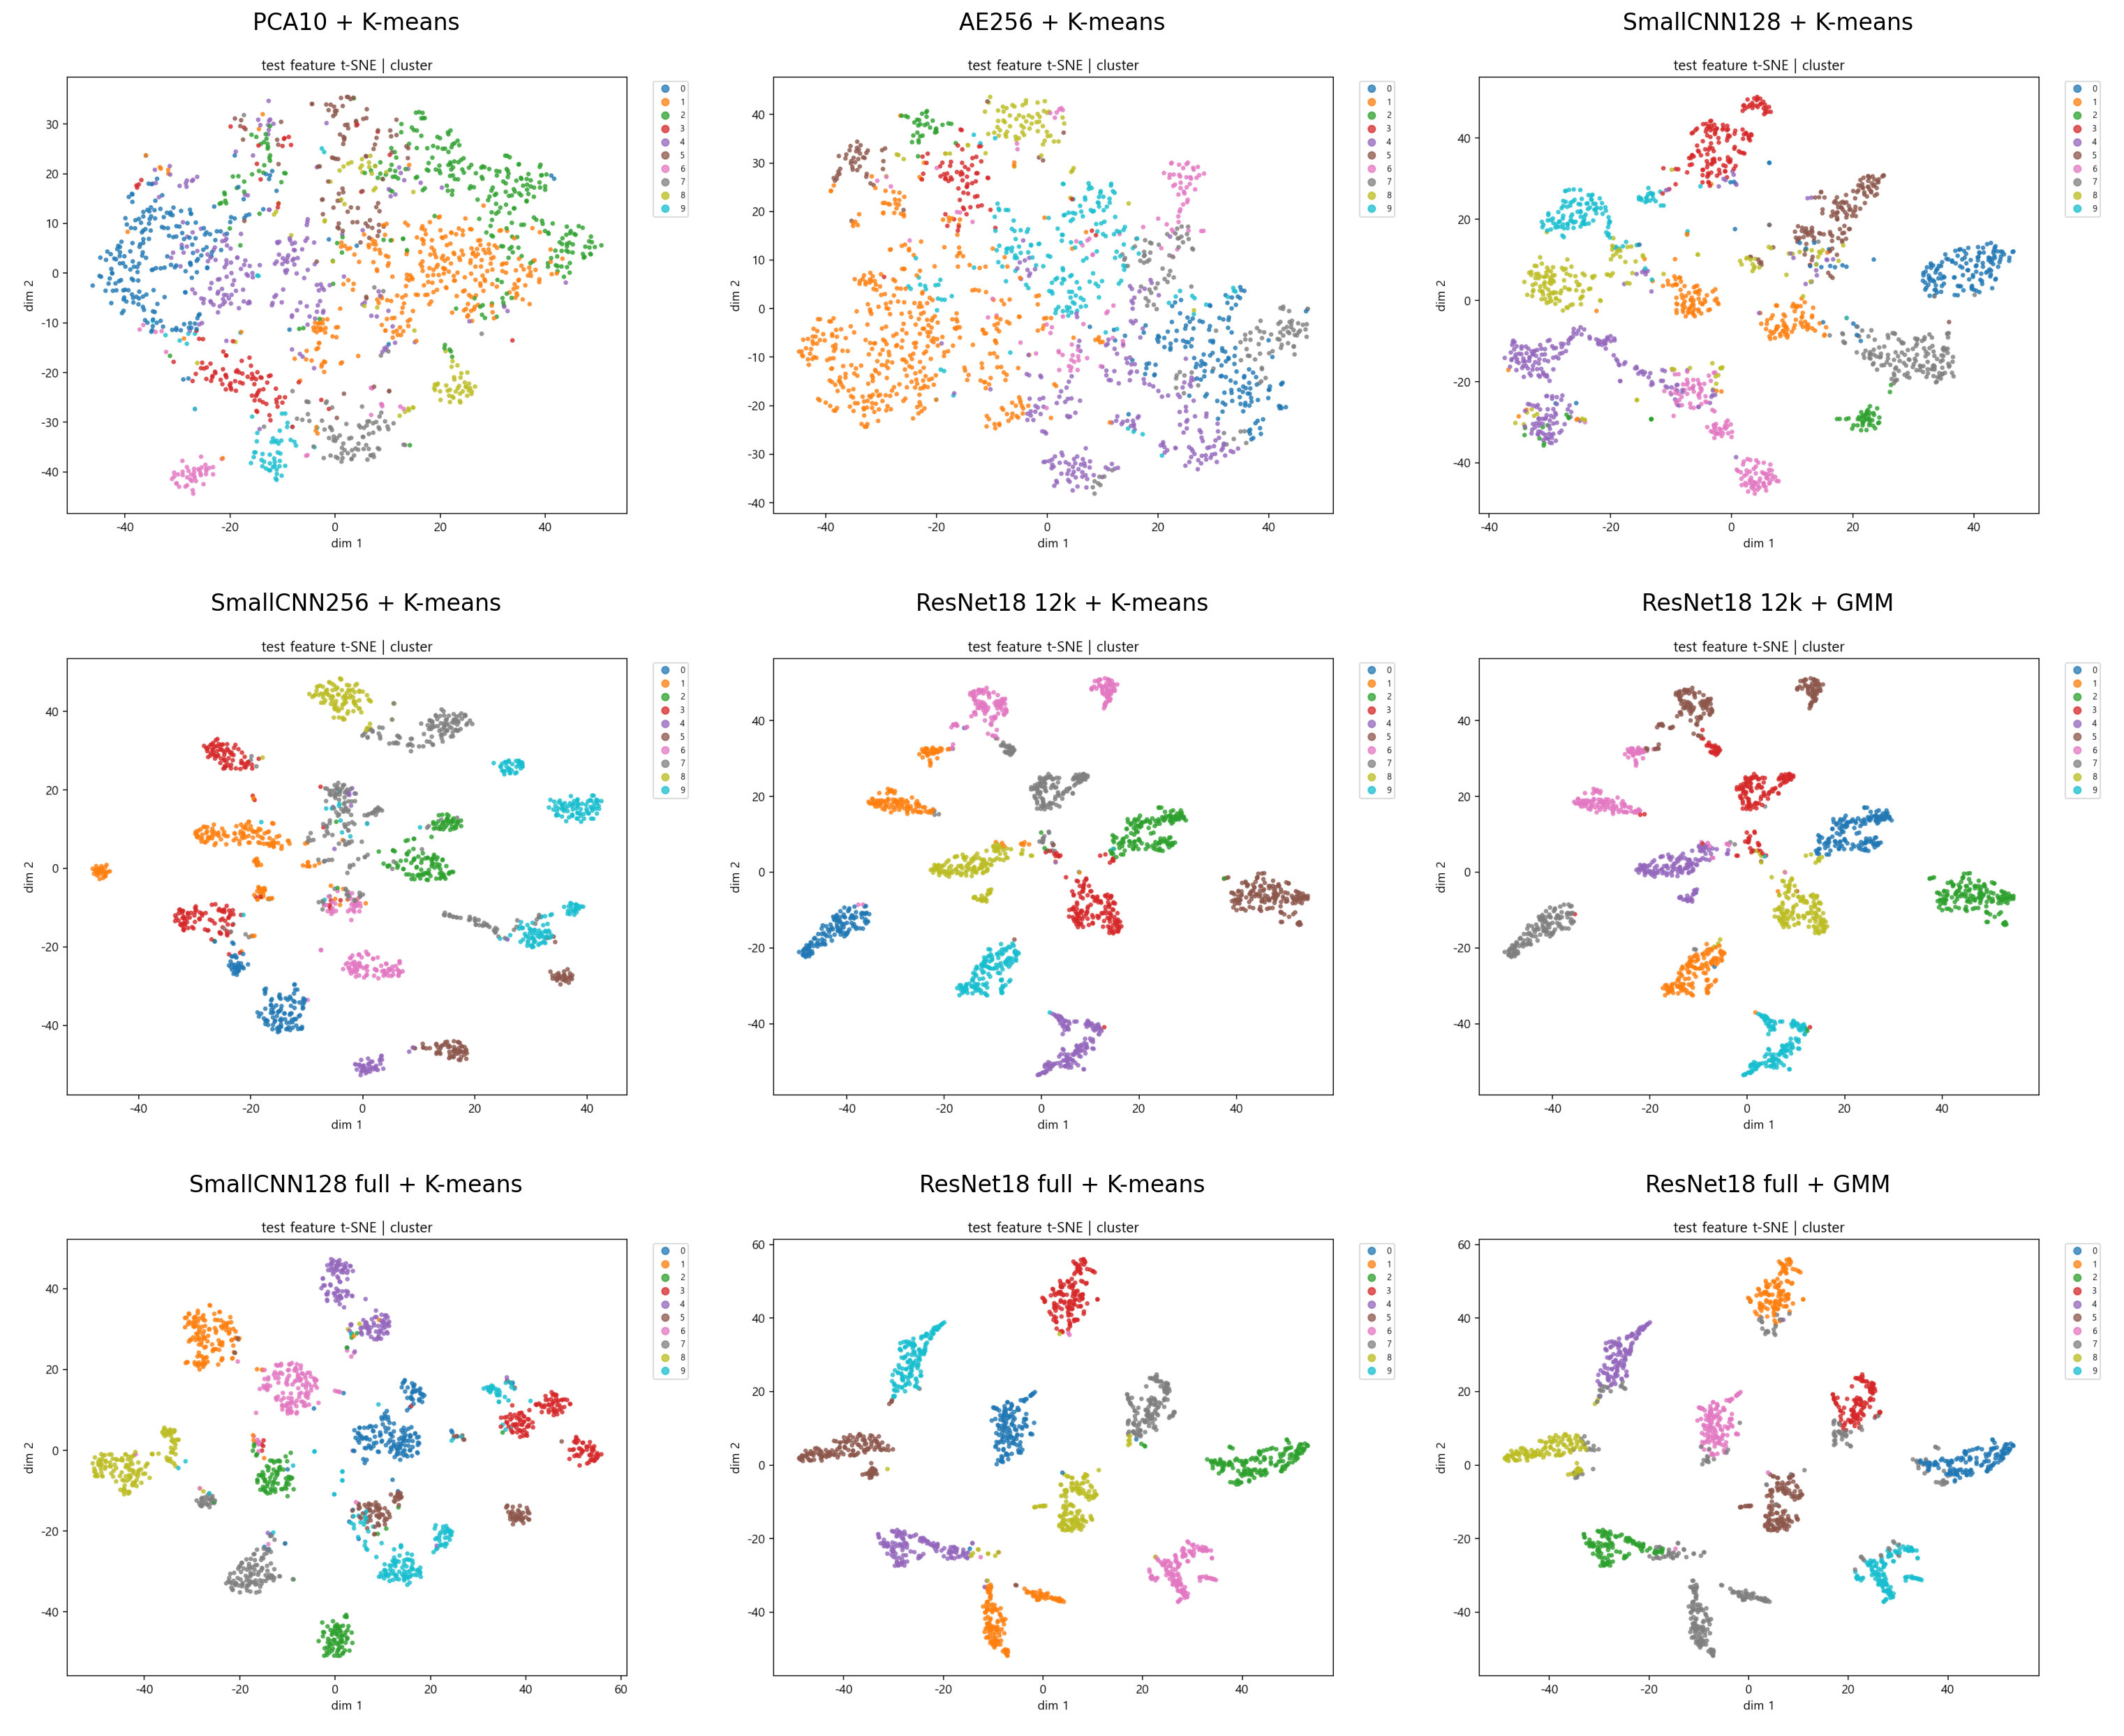
\includegraphics[width=\linewidth]{kmnist_all_runs_tsne_cluster.png}
    \caption{KMNIST t-SNE visualization by cluster for selected KMNIST runs. PCA and AE show mixed cluster structure, while CNN and especially ResNet18 produce clearer cluster islands.}
    \label{fig:kmnist-all-tsne}
\end{figure}

\begin{figure}[H]
    \centering
    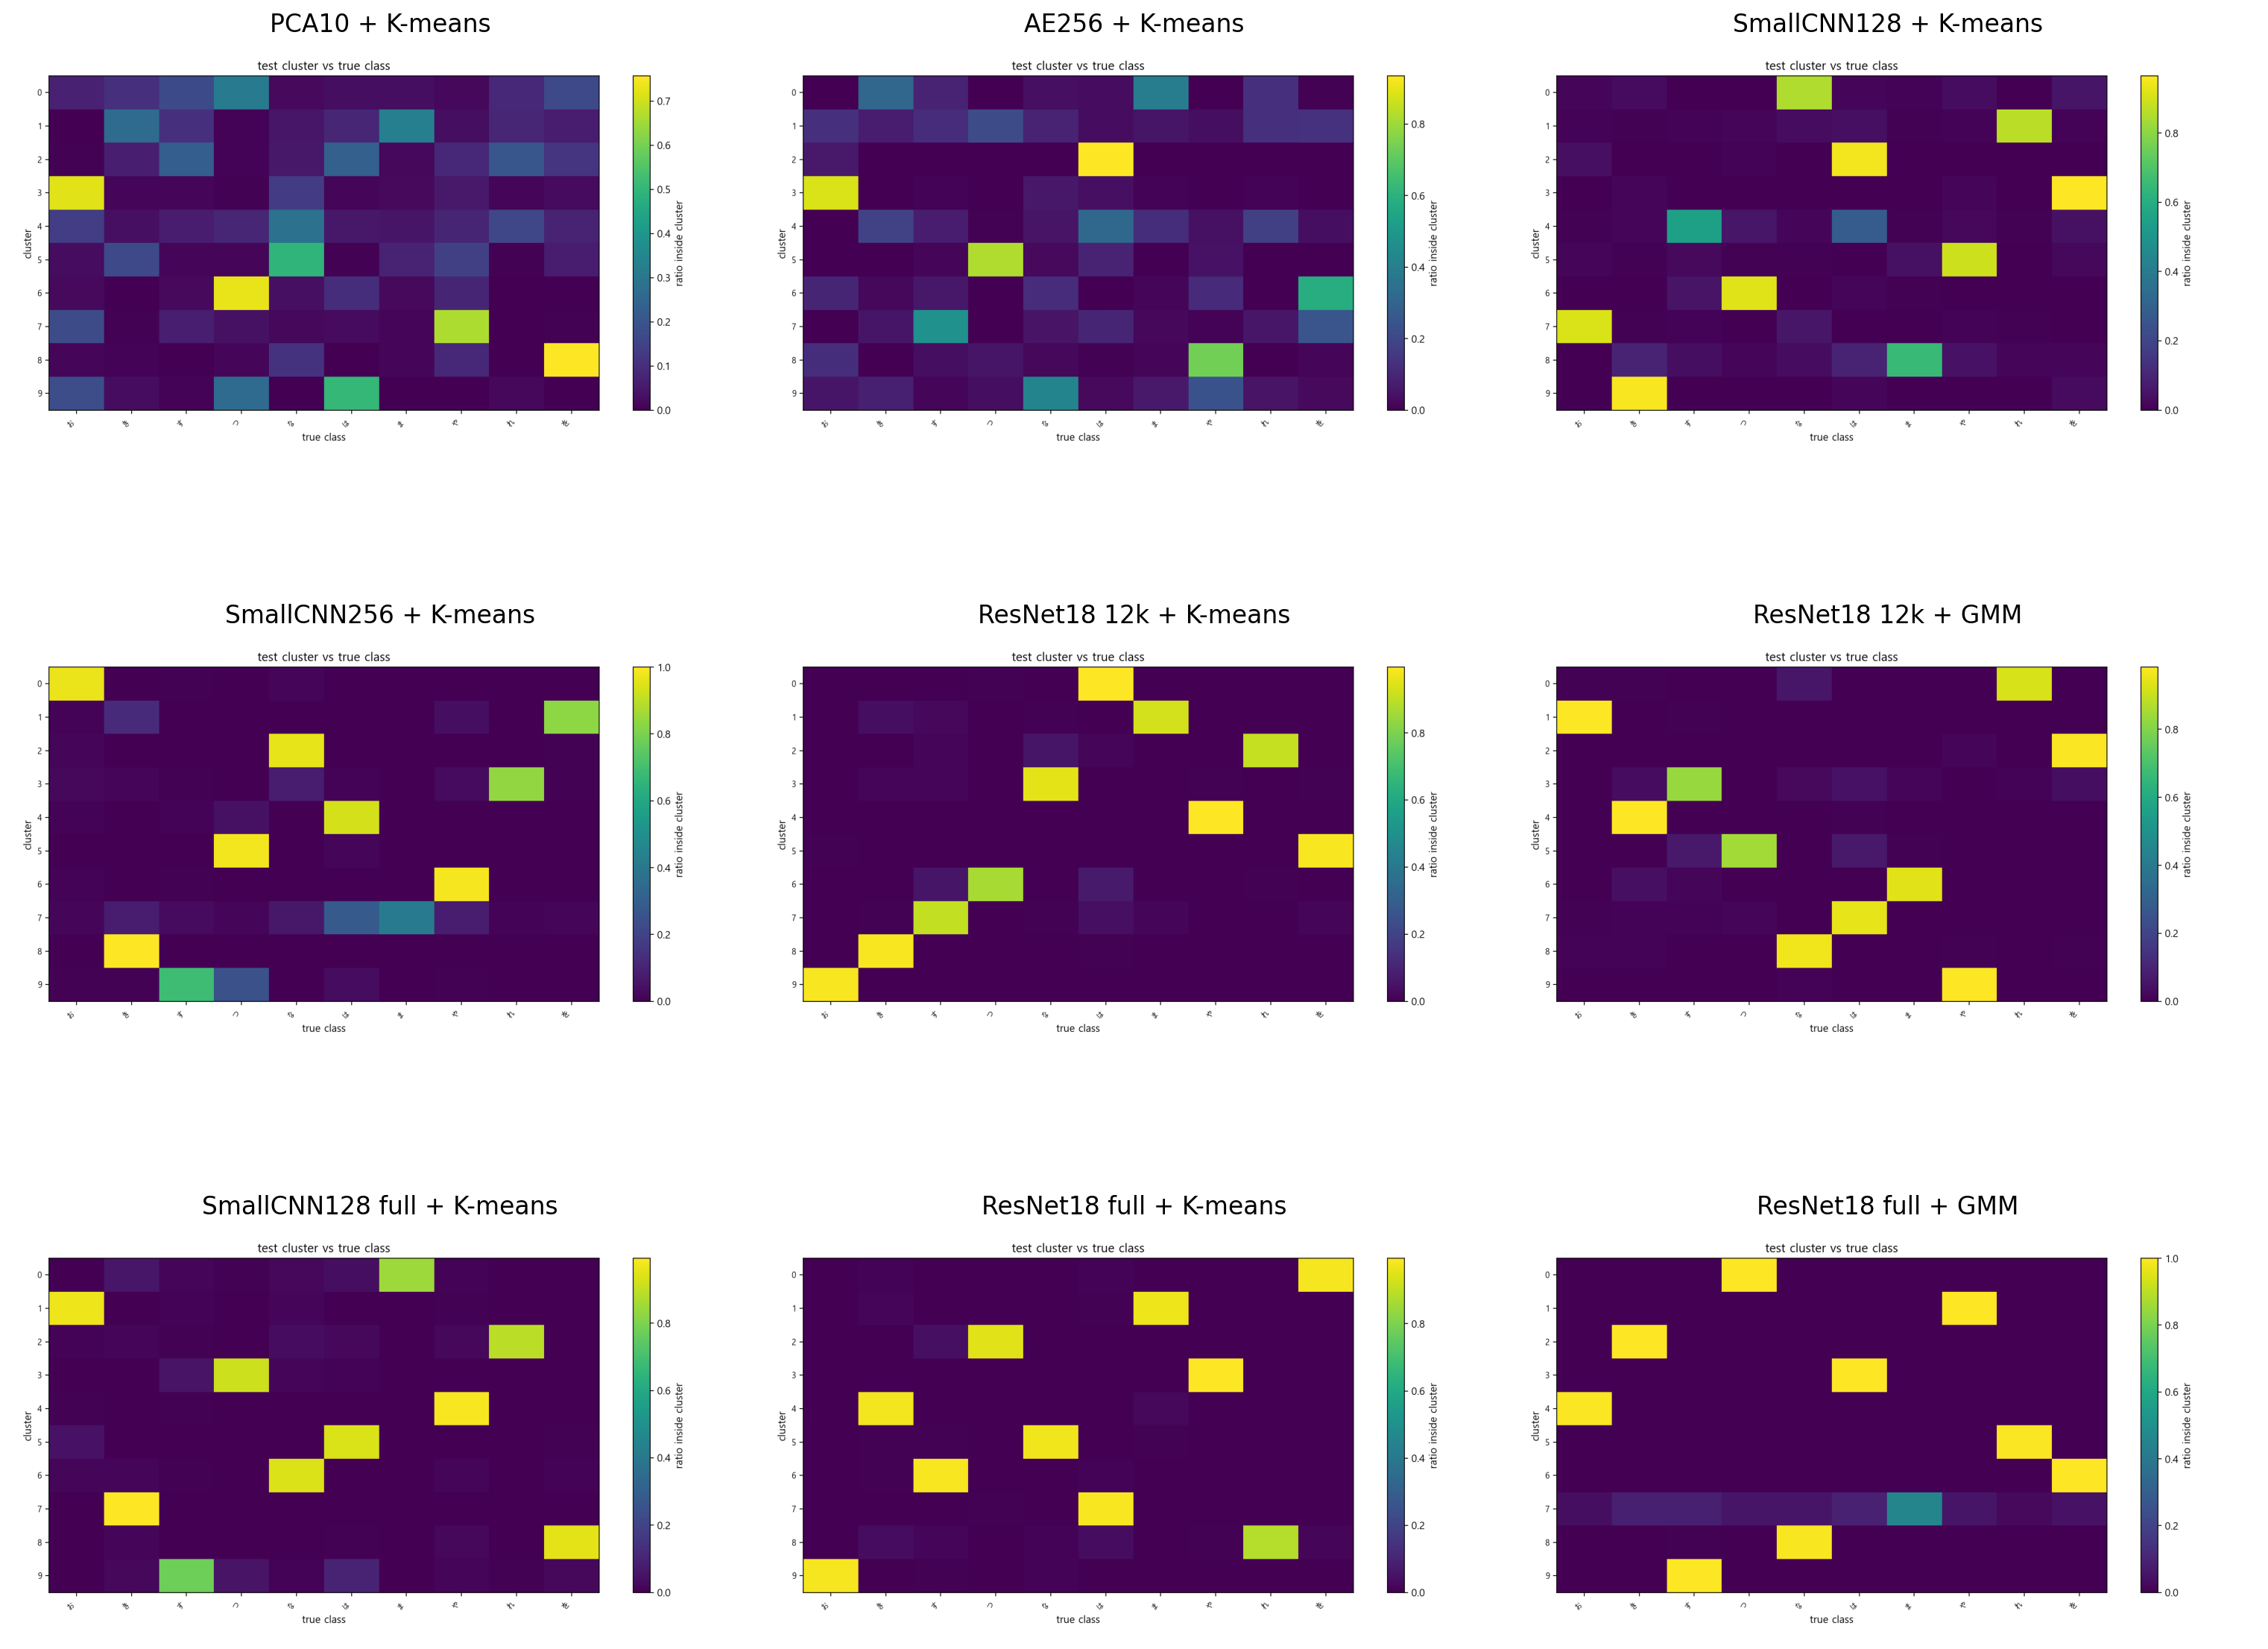
\includegraphics[width=\linewidth]{kmnist_all_runs_heatmaps.png}
    \caption{KMNIST cluster-class heatmaps for all KMNIST runs. Each row is a predicted cluster and each column is a true character class. Strong one-column concentration within each row indicates better class-level clustering.}
    \label{fig:kmnist-all-heatmaps}
\end{figure}

\subsection{Final Model Visual Analysis}

\subsubsection{t-SNE and Cluster-Class Heatmap}

Figure~\ref{fig:kmnist-tsne}는 ResNet18 + K-means full split 의 t-SNE visualization 이다.
True class 기준 그림과 cluster 기준 그림의 구조가 거의 대응된다.
일부 overlap 은 남아 있지만 대부분의 class 가 compact 한 island 로 분리되어 있으며, 이는 ARI/NMI 결과와 일치한다.

\begin{figure}[H]
    \centering
    \begin{subfigure}{0.48\linewidth}
        \centering
        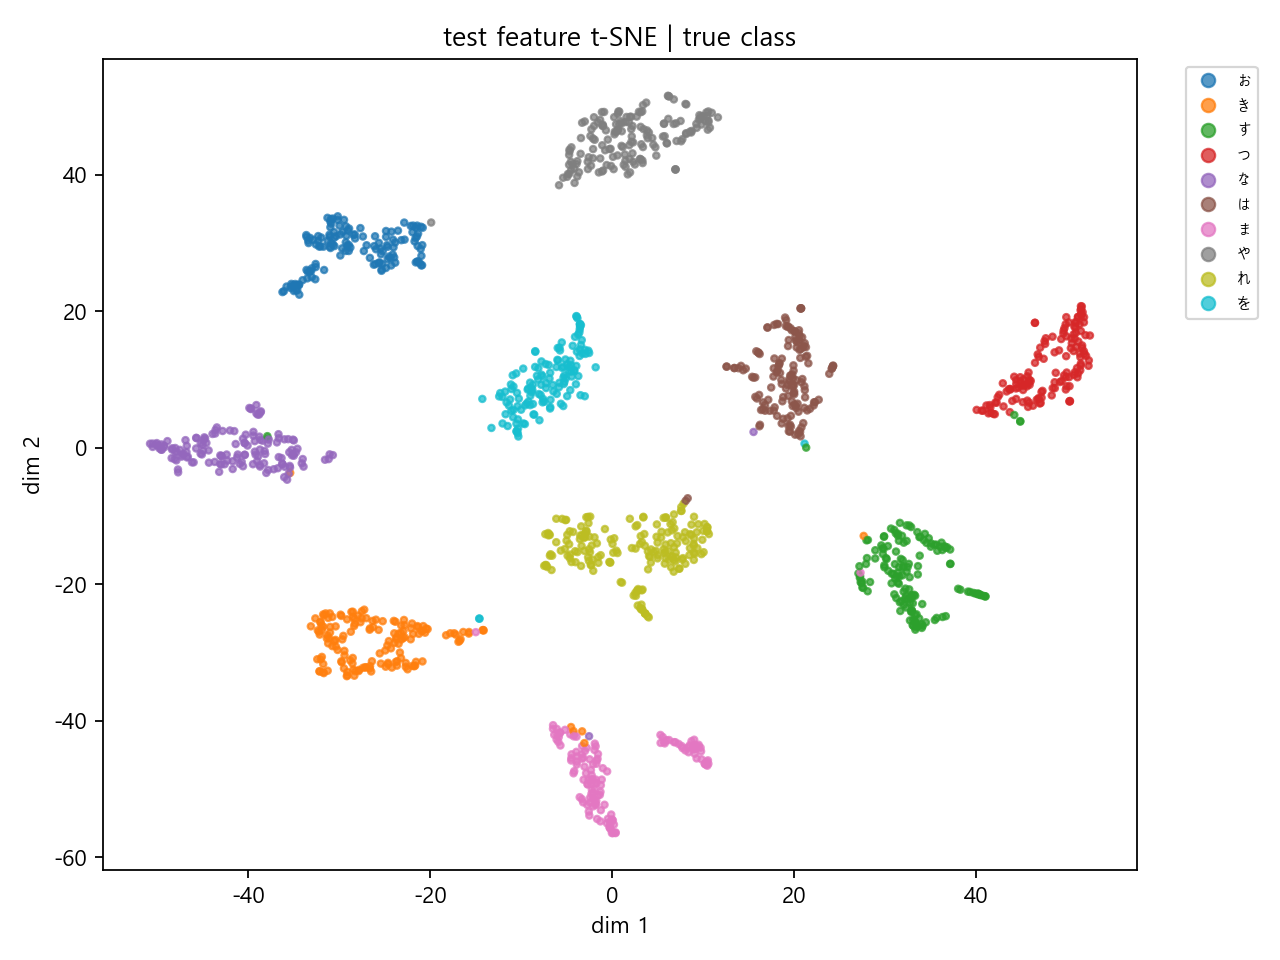
\includegraphics[width=\linewidth]{kmnist_resnet_kmeans_tsne_true.png}
        \caption{True class}
    \end{subfigure}
    \begin{subfigure}{0.48\linewidth}
        \centering
        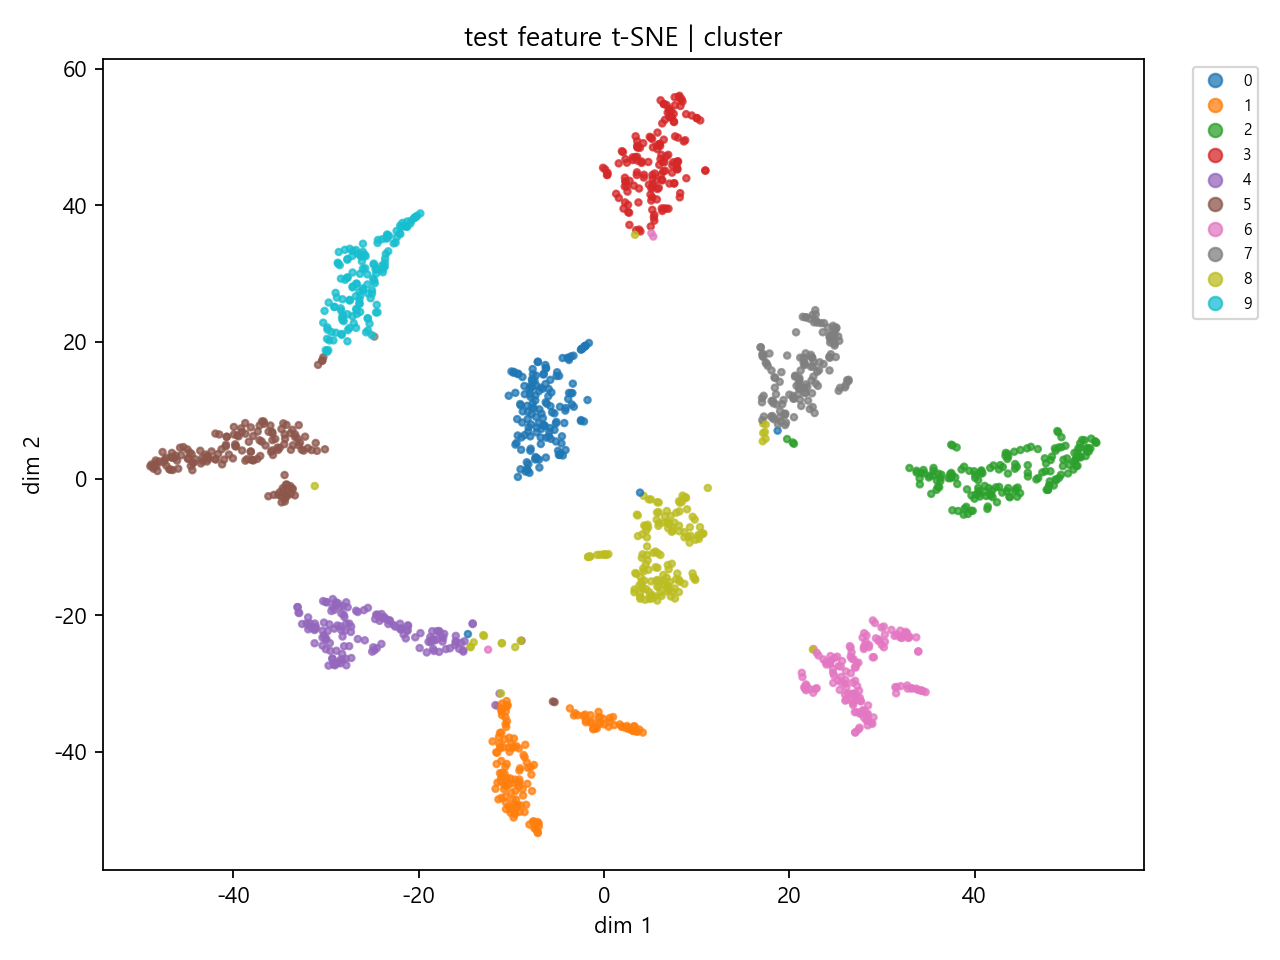
\includegraphics[width=\linewidth]{kmnist_resnet_kmeans_tsne_cluster.png}
        \caption{K-means cluster}
    \end{subfigure}
    \caption{KMNIST ResNet18 + K-means t-SNE visualization on the test set.}
    \label{fig:kmnist-tsne}
\end{figure}

Figure~\ref{fig:kmnist-heatmap}은 cluster-class heatmap 이다.
K-means 의 경우 각 cluster 행에서 count 가 특정 character class 열 하나에 강하게 집중되어, cluster 하나가 특정 class 하나와 거의 1:1로 대응된다.
반면 GMM 은 full ResNet feature 를 사용했음에도 cluster 하나가 여러 class 를 흡수하는 현상이 나타났다.
특히 GMM 에서는 여러 class 가 하나의 큰 component 로 들어가면서 ARI 가 0.7023 으로 낮아졌다.

\begin{figure}[H]
    \centering
    \begin{subfigure}{0.48\linewidth}
        \centering
        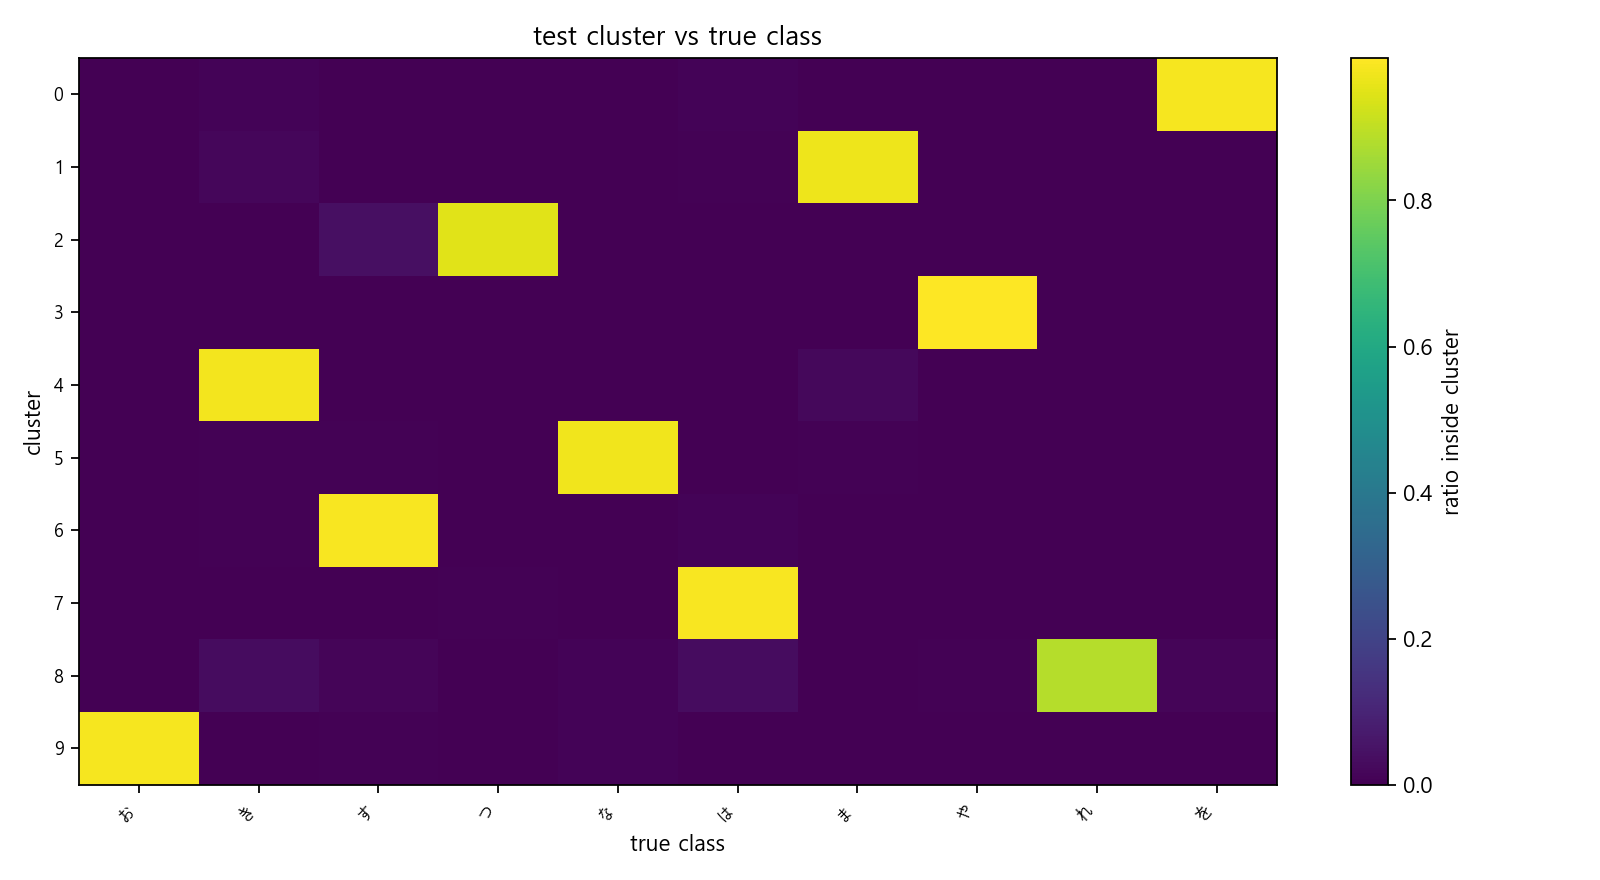
\includegraphics[width=\linewidth]{kmnist_resnet_kmeans_heatmap.png}
        \caption{K-means}
    \end{subfigure}
    \begin{subfigure}{0.48\linewidth}
        \centering
        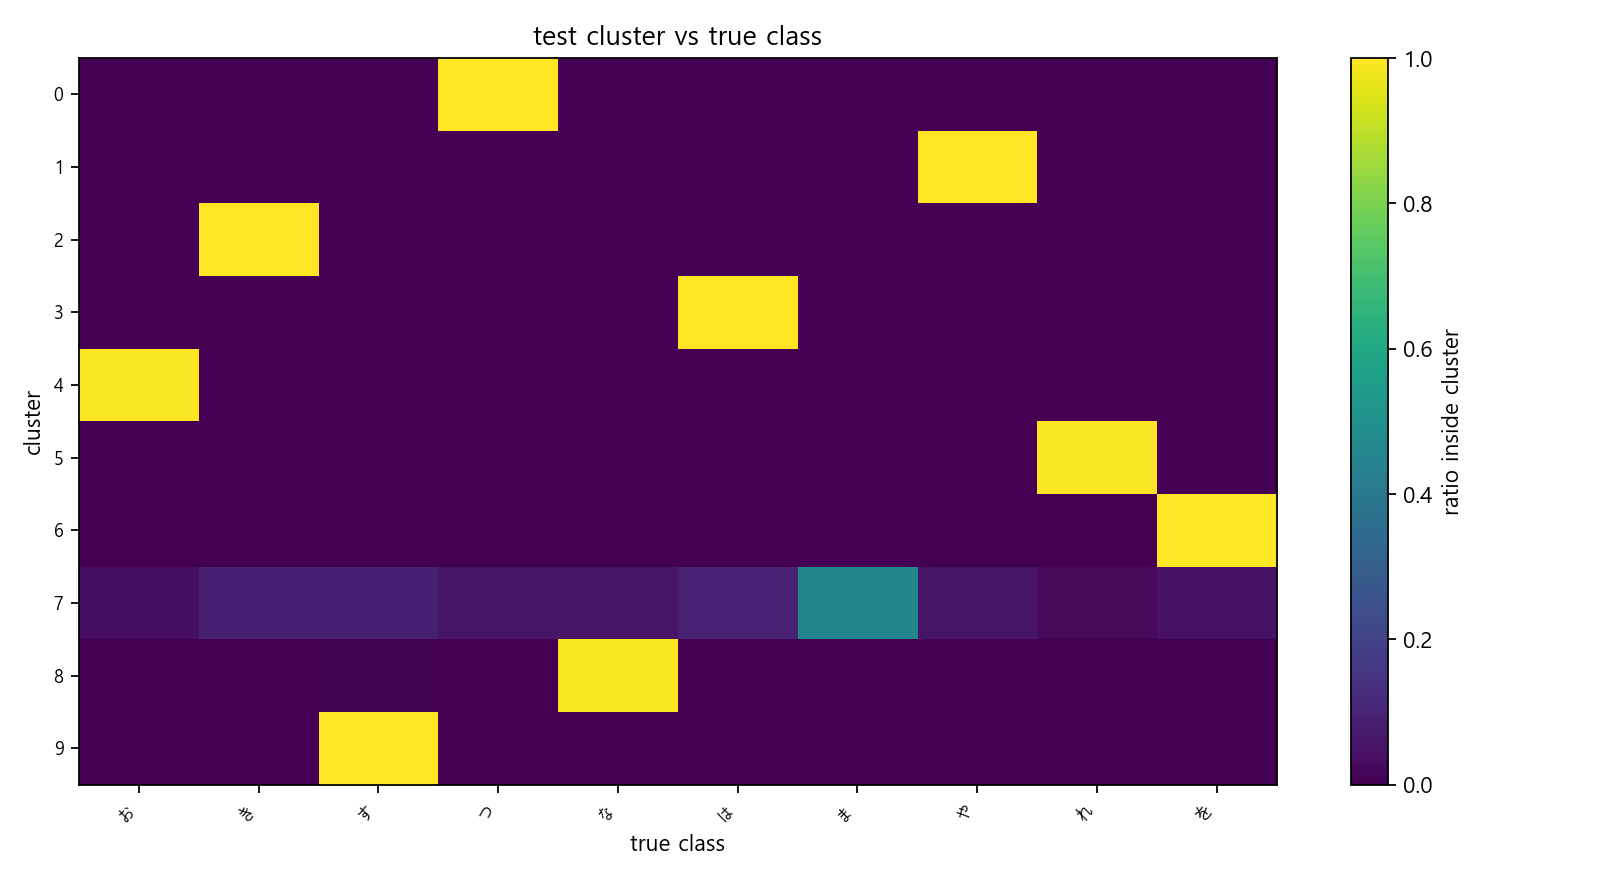
\includegraphics[width=\linewidth]{kmnist_resnet_gmm_heatmap.png}
        \caption{GMM}
    \end{subfigure}
    \caption{KMNIST cluster-class relationship for ResNet18 full-split features.}
    \label{fig:kmnist-heatmap}
\end{figure}

\subsubsection{Error Pattern}

Class별로 보면 ResNet18 + K-means 에서 문자 \jp{お}, \jp{つ}, \jp{や}, \jp{れ}, \jp{を} 는 dominant cluster ratio 가 0.98 이상으로 매우 잘 분리되었다.
상대적으로 자주 섞인 pair 는 \jp{す}\(\rightarrow\)\jp{つ}, \jp{き}\(\rightarrow\)\jp{れ}, \jp{は}\(\rightarrow\)\jp{れ} 등이었다.
이들은 획의 방향이나 stroke pattern 이 비슷하게 보이는 sample 에서 혼동이 발생하였다.

\begin{table}[H]
    \centering
    \caption{Most frequent KMNIST mapped-class mismatch pairs on the test set.}
    \label{tab:kmnist-mismatch-pairs}
    \small
    \begin{tabular}{llc}
        \toprule
        Run & True \(\rightarrow\) mapped class & Count\\
        \midrule
        ResNet18 + K-means full & \jp{す} \(\rightarrow\) \jp{つ} & 43\\
        ResNet18 + K-means full & \jp{き} \(\rightarrow\) \jp{れ} & 37\\
        ResNet18 + K-means full & \jp{は} \(\rightarrow\) \jp{れ} & 37\\
        ResNet18 + K-means full & \jp{ま} \(\rightarrow\) \jp{き} & 19\\
        ResNet18 + K-means full & \jp{す} \(\rightarrow\) \jp{れ} & 16\\
        \midrule
        ResNet18 + GMM full & \jp{は} \(\rightarrow\) \jp{ま} & 205\\
        ResNet18 + GMM full & \jp{す} \(\rightarrow\) \jp{ま} & 193\\
        ResNet18 + GMM full & \jp{き} \(\rightarrow\) \jp{ま} & 189\\
        ResNet18 + GMM full & \jp{な} \(\rightarrow\) \jp{ま} & 124\\
        ResNet18 + GMM full & \jp{や} \(\rightarrow\) \jp{ま} & 123\\
        \bottomrule
    \end{tabular}
\end{table}

Table~\ref{tab:kmnist-mismatch-pairs}에서 K-means 의 오인은 특정 pair 몇 개에 비교적 작게 집중된다.
반면 GMM 은 많은 class 를 \jp{ま}로 mapping 된 큰 component 에 넣는 경향이 강했다.
따라서 GMM 의 낮은 ARI 는 단순히 비슷한 문자 몇 개를 헷갈린 결과라기보다, component 하나가 여러 class 를 한꺼번에 흡수한 결과에 가깝다.

\begin{figure}[H]
    \centering
    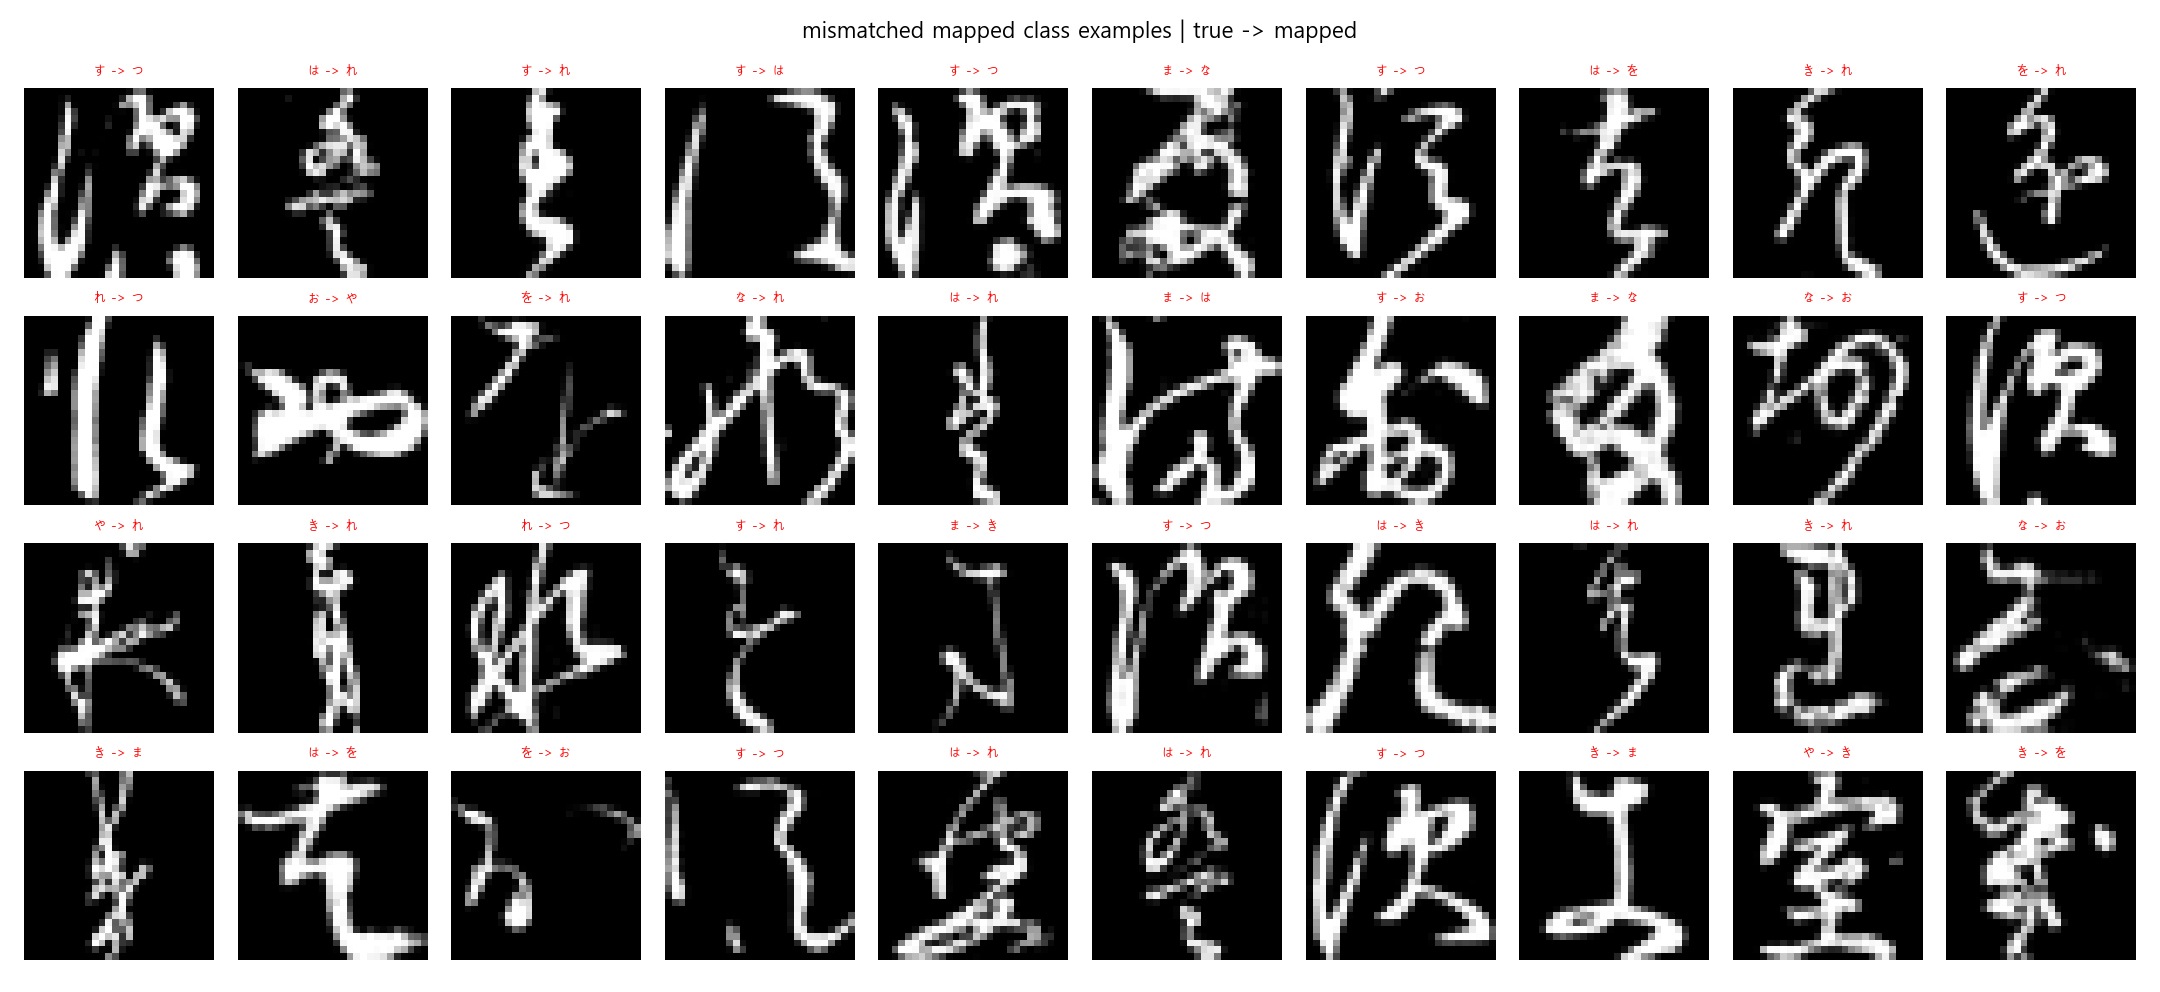
\includegraphics[width=0.82\linewidth]{kmnist_resnet_kmeans_mismatches.png}
    \caption{KMNIST examples whose true class and mapped cluster class differ.}
    \label{fig:kmnist-mismatch}
\end{figure}

\section{Results on CIFAR-10}

\subsection{Quantitative Results}

Table~\ref{tab:cifar-results}는 CIFAR-10 test set 결과이다.
PCA 와 AutoEncoder feature 는 CIFAR-10 에서 거의 class-level clustering 을 만들지 못했다.
PCA100 + K-means 는 ARI 0.0662, ConvAE64 + K-means 는 ARI 0.0548 이었다.
이는 raw pixel variance 또는 reconstruction objective 가 semantic class separation 과 직접적으로 일치하지 않기 때문이다.

\begin{table}[H]
    \centering
    \caption{CIFAR-10 test results.}
    \label{tab:cifar-results}
    \begin{tabular}{lccccc}
        \toprule
        Feature / clustering & Train size & ARI & NMI & Purity & Silhouette\\
        \midrule
        PCA100 + K-means & 12k & 0.0662 & 0.1320 & 0.2577 & -0.0483\\
        ConvAE64 + K-means & 12k & 0.0548 & 0.1130 & 0.2570 & 0.0535\\
        SmallCNN256 + K-means & 12k & 0.3527 & 0.5177 & 0.6320 & 0.1340\\
        ResNet18 + K-means & 12k & 0.3642 & 0.5543 & 0.6290 & 0.2177\\
        \textbf{ResNet18 + K-means} & \textbf{full} & \textbf{0.6408} & \textbf{0.7252} & \textbf{0.7825} & \textbf{0.2747}\\
        ResNet18 + GMM & full & 0.3178 & 0.5578 & 0.5434 & 0.1654\\
        \bottomrule
    \end{tabular}
\end{table}

CIFAR-10 에서는 feature extractor 의 구조와 train set 크기가 모두 중요했다.
PCA100 과 ConvAE64 는 ARI 0.07 이하에 머물렀고, supervised CNN feature 를 사용한 뒤에야 ARI 가 0.35 이상으로 올라갔다.
다만 SmallCNN256 과 ResNet18 은 12k subset 에서는 ARI 차이가 작았다.
ResNet18 을 full train split 으로 학습했을 때 ARI 가 0.6408 로 크게 상승한 점을 보면, CIFAR-10 에서는 모델을 키우는 것만으로는 부족하고 충분한 sample 로 feature extractor 를 학습해야 했다.

\subsubsection{PCA and AutoEncoder Features}

CIFAR-10 에서 PCA100 + K-means 는 ARI 0.0662, purity 0.2577 이었다.
KMNIST 와 달리 CIFAR-10 은 RGB image 이고, 같은 class 안에서도 배경, object 위치, pose, texture 가 많이 달라진다.
PCA 는 이런 pixel-level variance 를 잘 요약하지만, 그 방향이 semantic class 와 일치한다고 보장할 수 없다.
실제로 PCA100 run 에서는 airplane, bird, cat, deer, horse 등이 dog 또는 airplane 으로 자주 mapping 되었고, class별 dominant cluster ratio 도 대부분 0.20--0.49 수준에 머물렀다.

\begin{figure}[H]
    \centering
    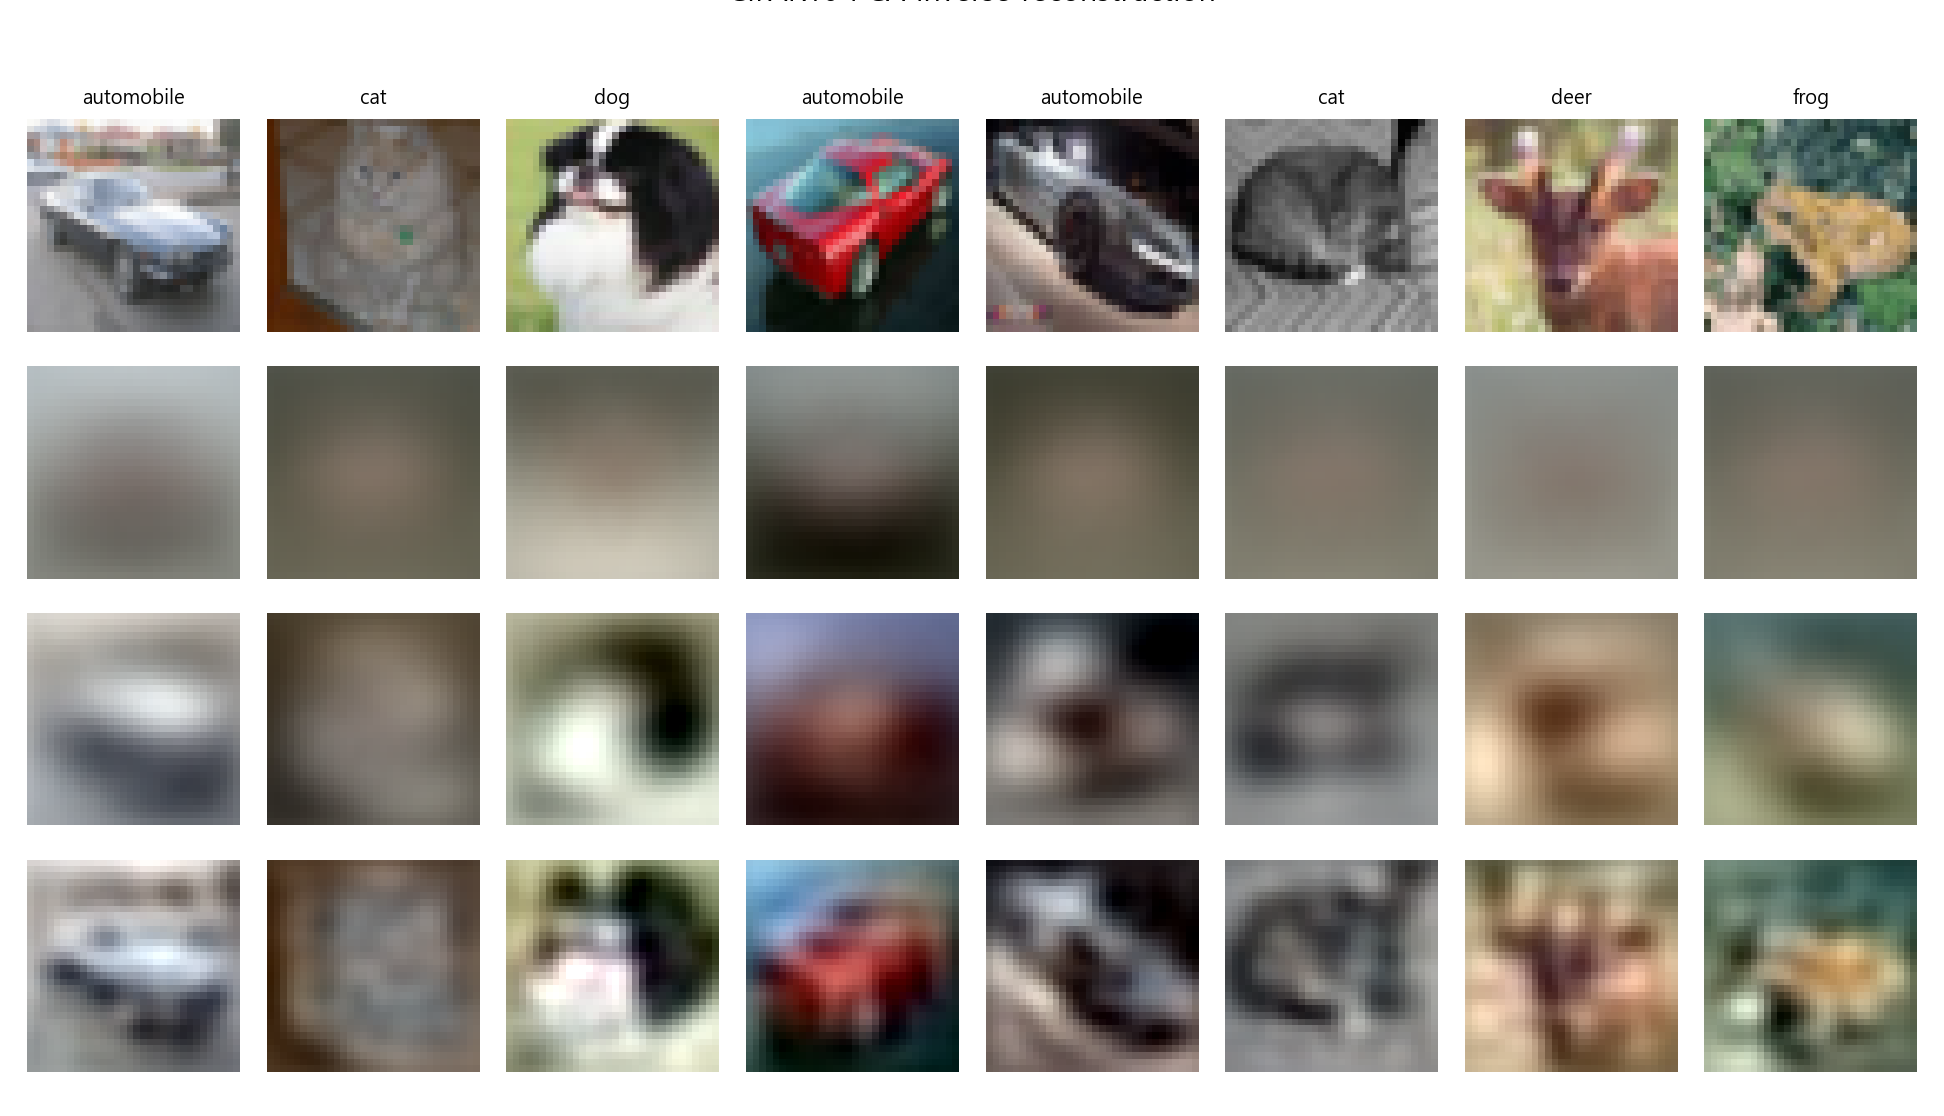
\includegraphics[width=0.92\linewidth]{cifar10_pca100_kmeans_pca_reconstruction.png}
    \caption{CIFAR-10 PCA inverse reconstruction examples. PCA preserves coarse color and layout, but fine object boundary and texture are blurred.}
    \label{fig:cifar-pca-reconstruction}
\end{figure}

Figure~\ref{fig:cifar-pca-reconstruction}에서 PCA reconstruction 은 색감과 큰 배치는 어느 정도 복원하지만, object boundary 와 texture 가 흐릿하다.
이 정도 정보만으로는 cat 과 dog, bird 와 airplane, ship 과 airplane 처럼 배경이나 윤곽이 겹치는 class 를 안정적으로 나누기 어렵다.

ConvAE64 + K-means 도 ARI 0.0548 로 PCA 보다 좋아지지 않았다.
AutoEncoder 는 reconstruction loss 를 줄이도록 학습되므로, 배경색과 전체적인 형태를 복원하는 데 필요한 정보는 latent vector 에 남긴다.
하지만 class separation 을 직접 요구하지 않기 때문에, latent space 에서 cluster 가 생기더라도 그 cluster 가 CIFAR-10 class 와 대응되지는 않았다.

\begin{figure}[H]
    \centering
    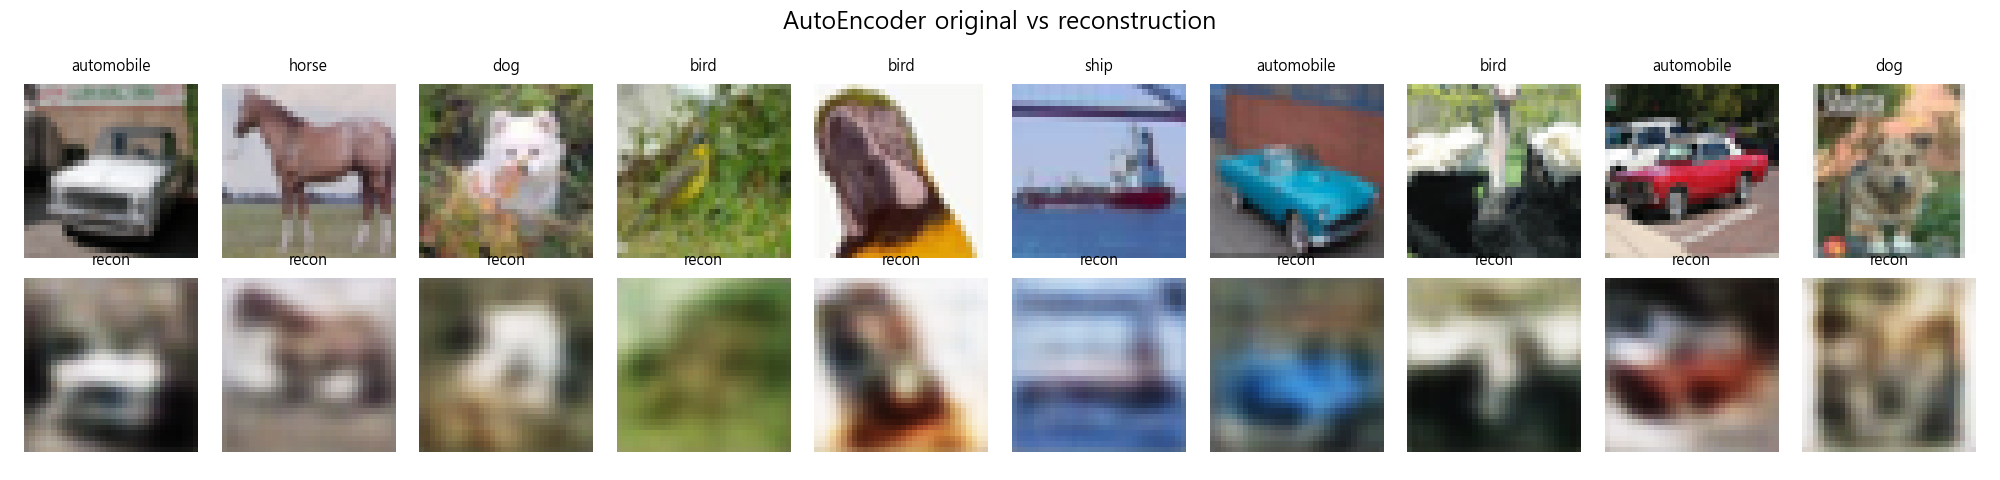
\includegraphics[width=0.86\linewidth]{cifar10_ae_reconstruction_grid.png}
    \caption{CIFAR-10 AutoEncoder reconstruction examples. Reconstructions keep coarse color and object placement, but object identity is often blurred.}
    \label{fig:cifar-ae-reconstruction}
\end{figure}

Figure~\ref{fig:cifar-ae-reconstruction}에서도 복원 이미지는 원본의 큰 색상과 위치는 유지하지만 object identity 는 많이 흐려진다.
따라서 ConvAE latent feature 는 image compression feature 로는 의미가 있지만, 본 실험의 class-level clustering feature 로는 충분하지 않았다.

\subsubsection{SmallCNN Features}

SmallCNN256 + K-means 는 ARI 0.3527, NMI 0.5177, purity 0.6320 으로 PCA/AE 보다 크게 좋아졌다.
이 run 은 wider channel \([64,128,256]\), embedding 256, dropout 0.25, normalization, random crop, horizontal flip 을 사용한 설정이다.
Supervised classifier 로 먼저 학습했기 때문에 class label 과 관련된 feature 를 만들 수 있었고, 그 결과 t-SNE plot 에서도 PCA/AE 보다 cluster island 가 뚜렷해졌다.

하지만 class별 결과를 보면 여전히 한계가 뚜렷하다.
Automobile 과 ship 은 dominant cluster ratio 가 각각 0.802, 0.825 로 비교적 높았지만, bird 는 0.444, cat 은 0.516, horse 는 0.547 에 그쳤다.
주요 오인은 cat \(\rightarrow\) dog 100개, horse \(\rightarrow\) cat 98개, dog \(\rightarrow\) cat 97개, bird \(\rightarrow\) cat 89개였다.
즉 SmallCNN feature 는 큰 object category 를 어느 정도 나누지만, 동물 class 내부의 pose 와 texture 차이를 충분히 정리하지 못했다.

\subsubsection{ResNet18 Features}

ResNet18 + K-means 는 12k subset 에서 ARI 0.3642 로 SmallCNN256 의 0.3527 보다 조금 높았다.
차이가 작아 보이지만 NMI 는 0.5177 에서 0.5543 으로, silhouette 은 0.1340 에서 0.2177 로 올라갔다.
이는 12k subset 에서도 ResNet18 feature space 가 geometric cluster 를 더 뚜렷하게 만들기 시작했다는 뜻이다.

Full train split 을 사용하면 차이가 훨씬 커졌다.
ResNet18 + K-means full run 은 ARI 0.6408, NMI 0.7252, purity 0.7825 를 얻었다.
Class별 dominant cluster ratio 는 airplane 0.956, automobile 0.944, dog 0.930, frog 0.905, truck 0.895, ship 0.868 로 높았다.
상대적으로 낮은 class 는 bird 0.642, horse 0.818, cat 0.842 였다.
이는 CIFAR-10 에서도 man-made object 나 배경이 비교적 일정한 class 는 잘 모이지만, 동물 class 와 작은 object class 는 더 어렵다는 점을 보여준다.

\begin{figure}[H]
    \centering
    \begin{subfigure}{0.92\linewidth}
        \centering
        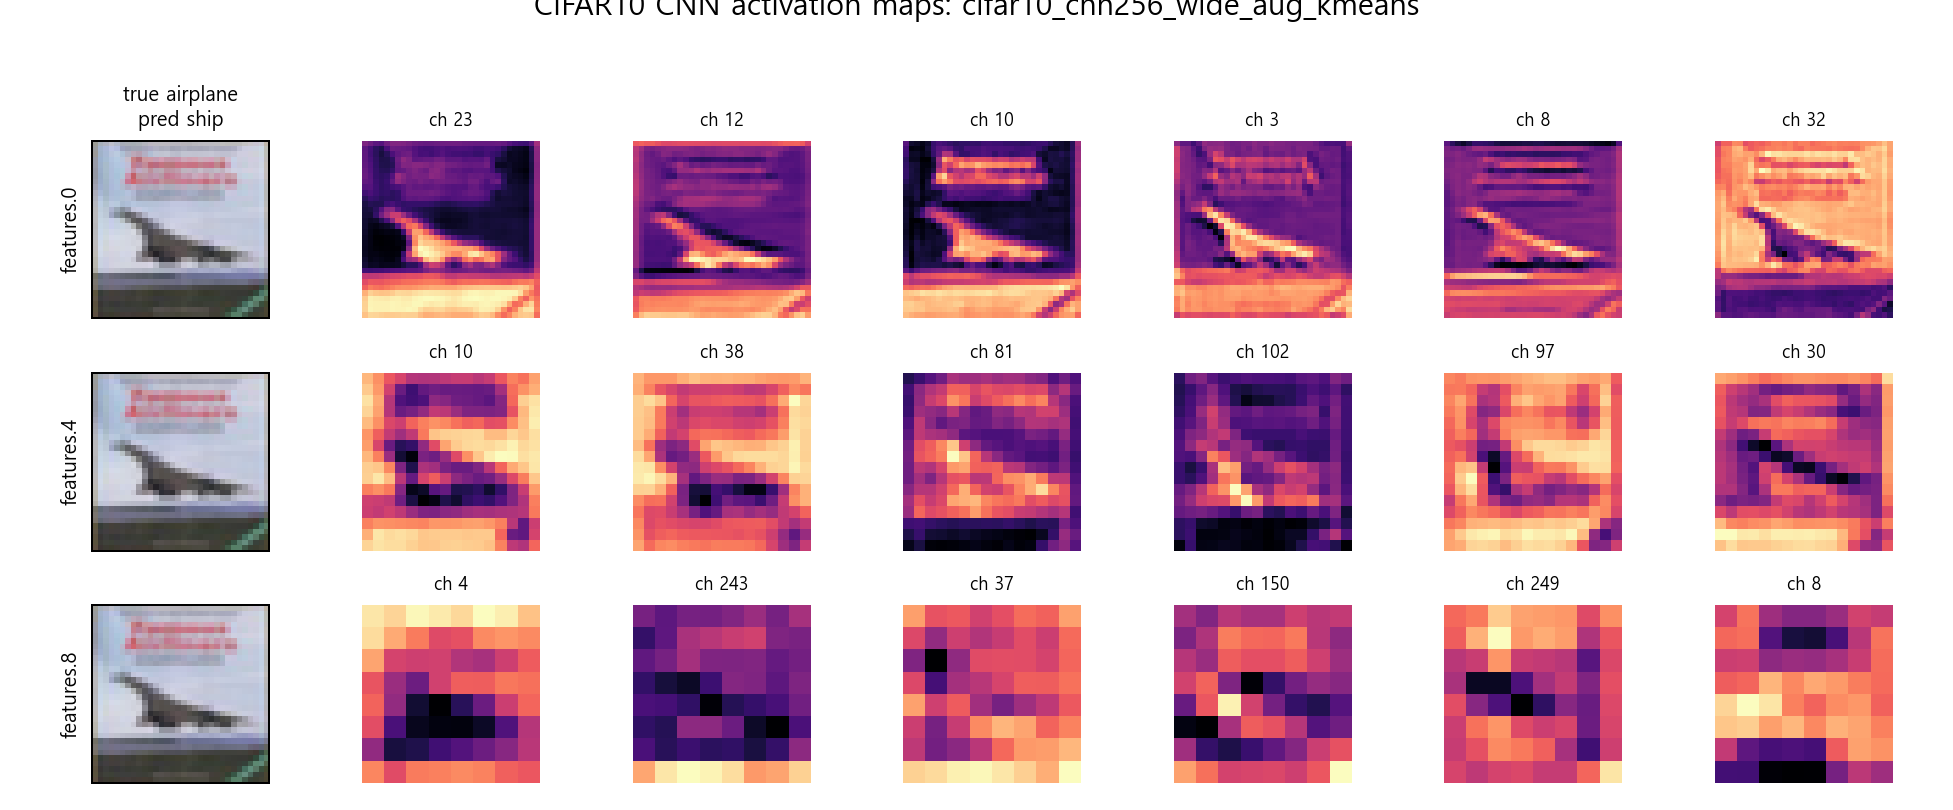
\includegraphics[width=\linewidth]{cifar10_cnn256_wide_aug_kmeans_activation_maps.png}
        \caption{SmallCNN256}
    \end{subfigure}
    \vspace{0.08in}
    \begin{subfigure}{0.92\linewidth}
        \centering
        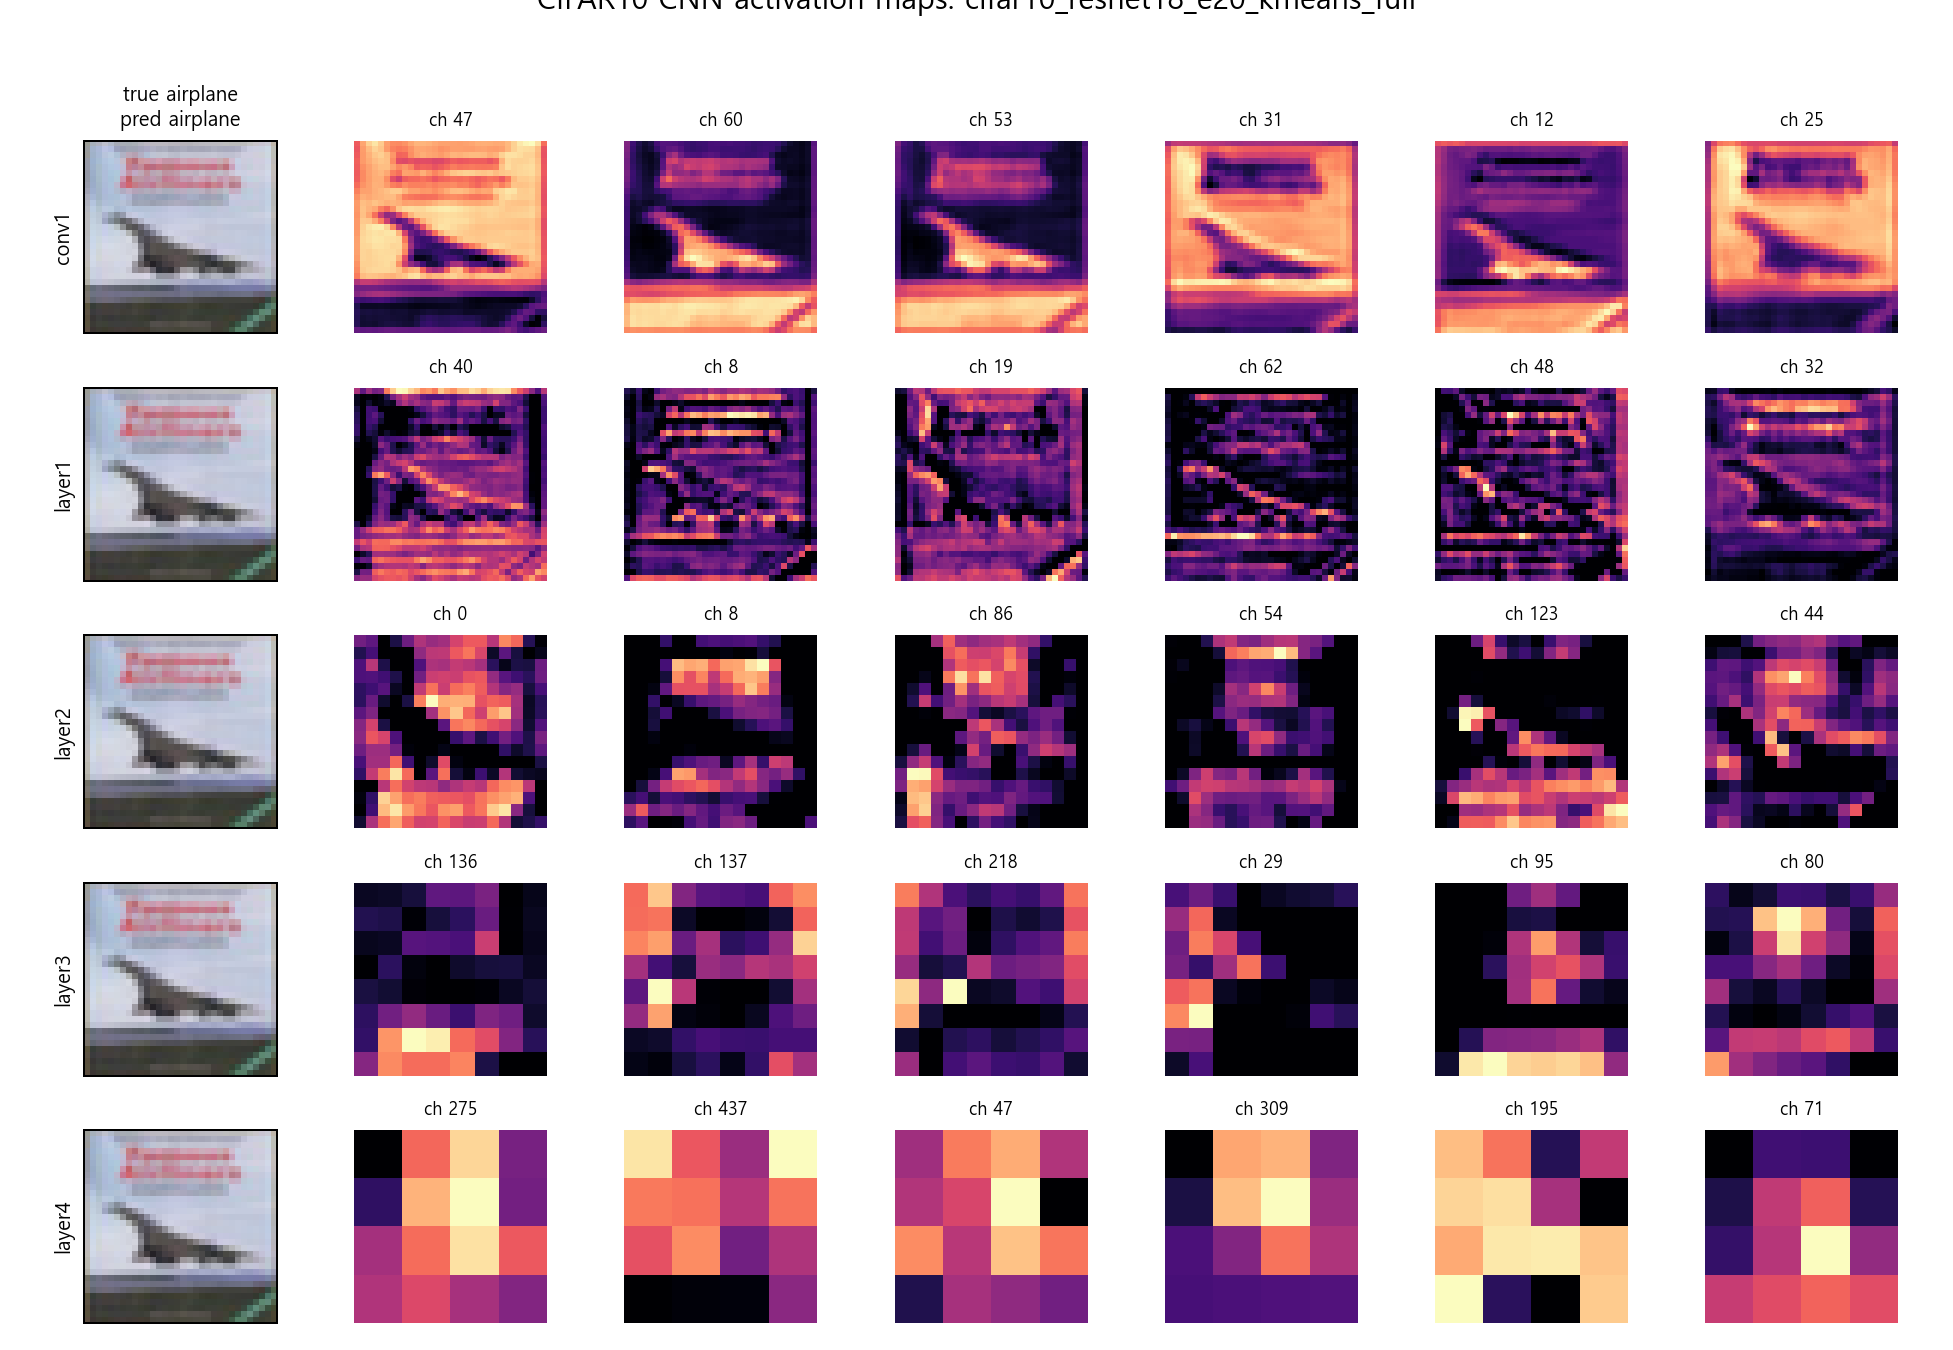
\includegraphics[width=\linewidth]{cifar10_resnet18_e20_kmeans_full_activation_maps.png}
        \caption{ResNet18}
    \end{subfigure}
    \caption{CIFAR-10 CNN activation maps for the same raw test image. The true class is airplane; SmallCNN predicts ship, while ResNet18 predicts airplane.}
    \label{fig:cifar-cnn-activation}
\end{figure}

Figure~\ref{fig:cifar-cnn-activation}은 같은 airplane image 를 SmallCNN 과 ResNet18 에 넣고 activation map 을 비교한 것이다.
SmallCNN 은 초반 layer 에서 airplane 과 배경의 horizontal edge 에 반응하지만, 뒤쪽 feature map 에서 전체 image 가 긴 horizontal pattern 중심으로 압축되어 classifier prediction 이 ship 으로 나왔다.
ResNet18 도 초반에는 같은 edge 와 texture 에 반응하지만, 더 깊은 layer 에서 object 영역과 배경이 구분되는 activation 이 더 오래 남아 있고 최종적으로 airplane 으로 맞혔다.
이 example 은 CIFAR-10 에서 단순한 윤곽 정보만으로는 class 를 구분하기 어렵고, 더 깊은 feature hierarchy 가 필요한 경우를 보여준다.

\subsubsection{K-means and GMM Comparison}

CIFAR-10 에서도 GMM 은 K-means 보다 낮았다.
같은 ResNet18 full feature 를 사용했을 때 K-means 는 ARI 0.6408 이었지만, GMM 은 ARI 0.3178 로 떨어졌다.
GMM full run 에서는 test set 10,000개 중 cluster 9 가 3,863개, cluster 3 이 2,026개를 차지했고, 하나의 큰 component 가 여러 class 를 흡수했다.
예를 들어 cat 929개, deer 961개, dog 768개가 같은 component 쪽으로 묶이는 현상이 나타났다.
이는 CIFAR-10 CNN embedding 이 diagonal Gaussian mixture 로 깔끔하게 나뉘지 않았기 때문으로 볼 수 있다.

\subsubsection{All-run Visual Comparison}

\begin{figure}[H]
    \centering
    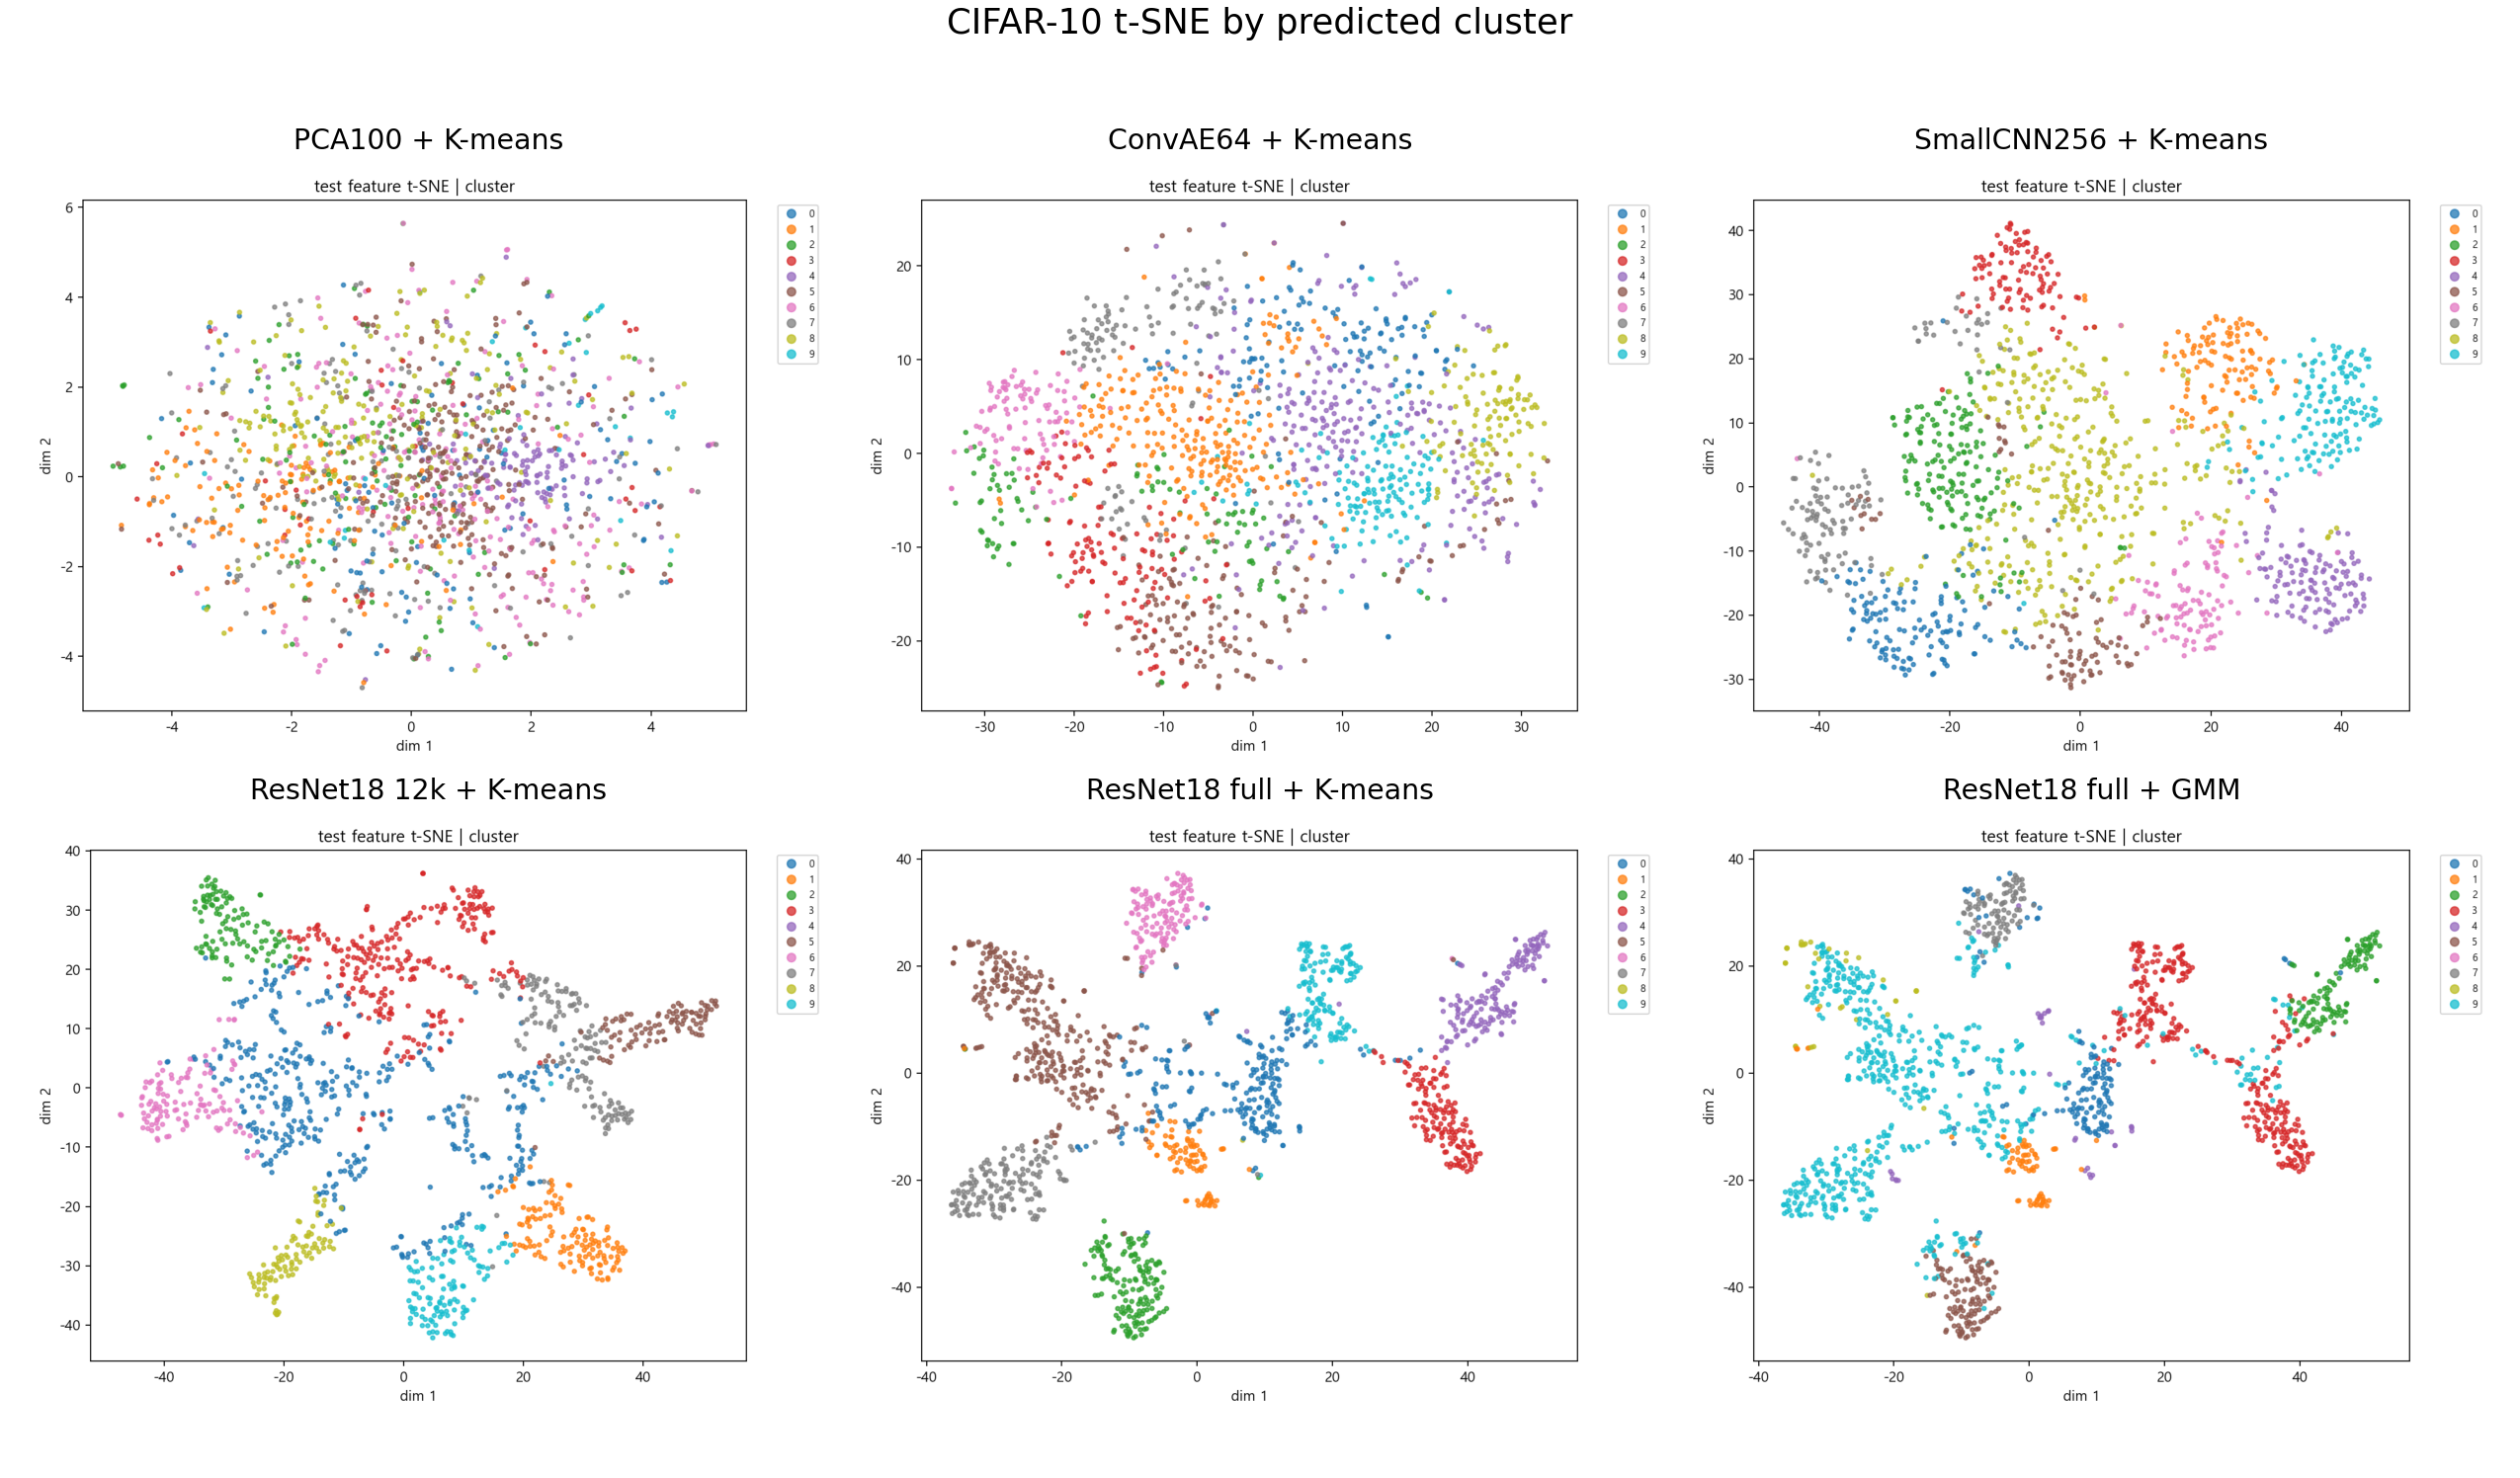
\includegraphics[width=\linewidth]{cifar10_all_runs_tsne_cluster.png}
    \caption{CIFAR-10 t-SNE visualization by cluster for selected CIFAR-10 runs. PCA and AE remain mixed, SmallCNN begins to form islands, and ResNet18 full training produces the clearest cluster structure.}
    \label{fig:cifar-all-tsne}
\end{figure}

\begin{figure}[H]
    \centering
    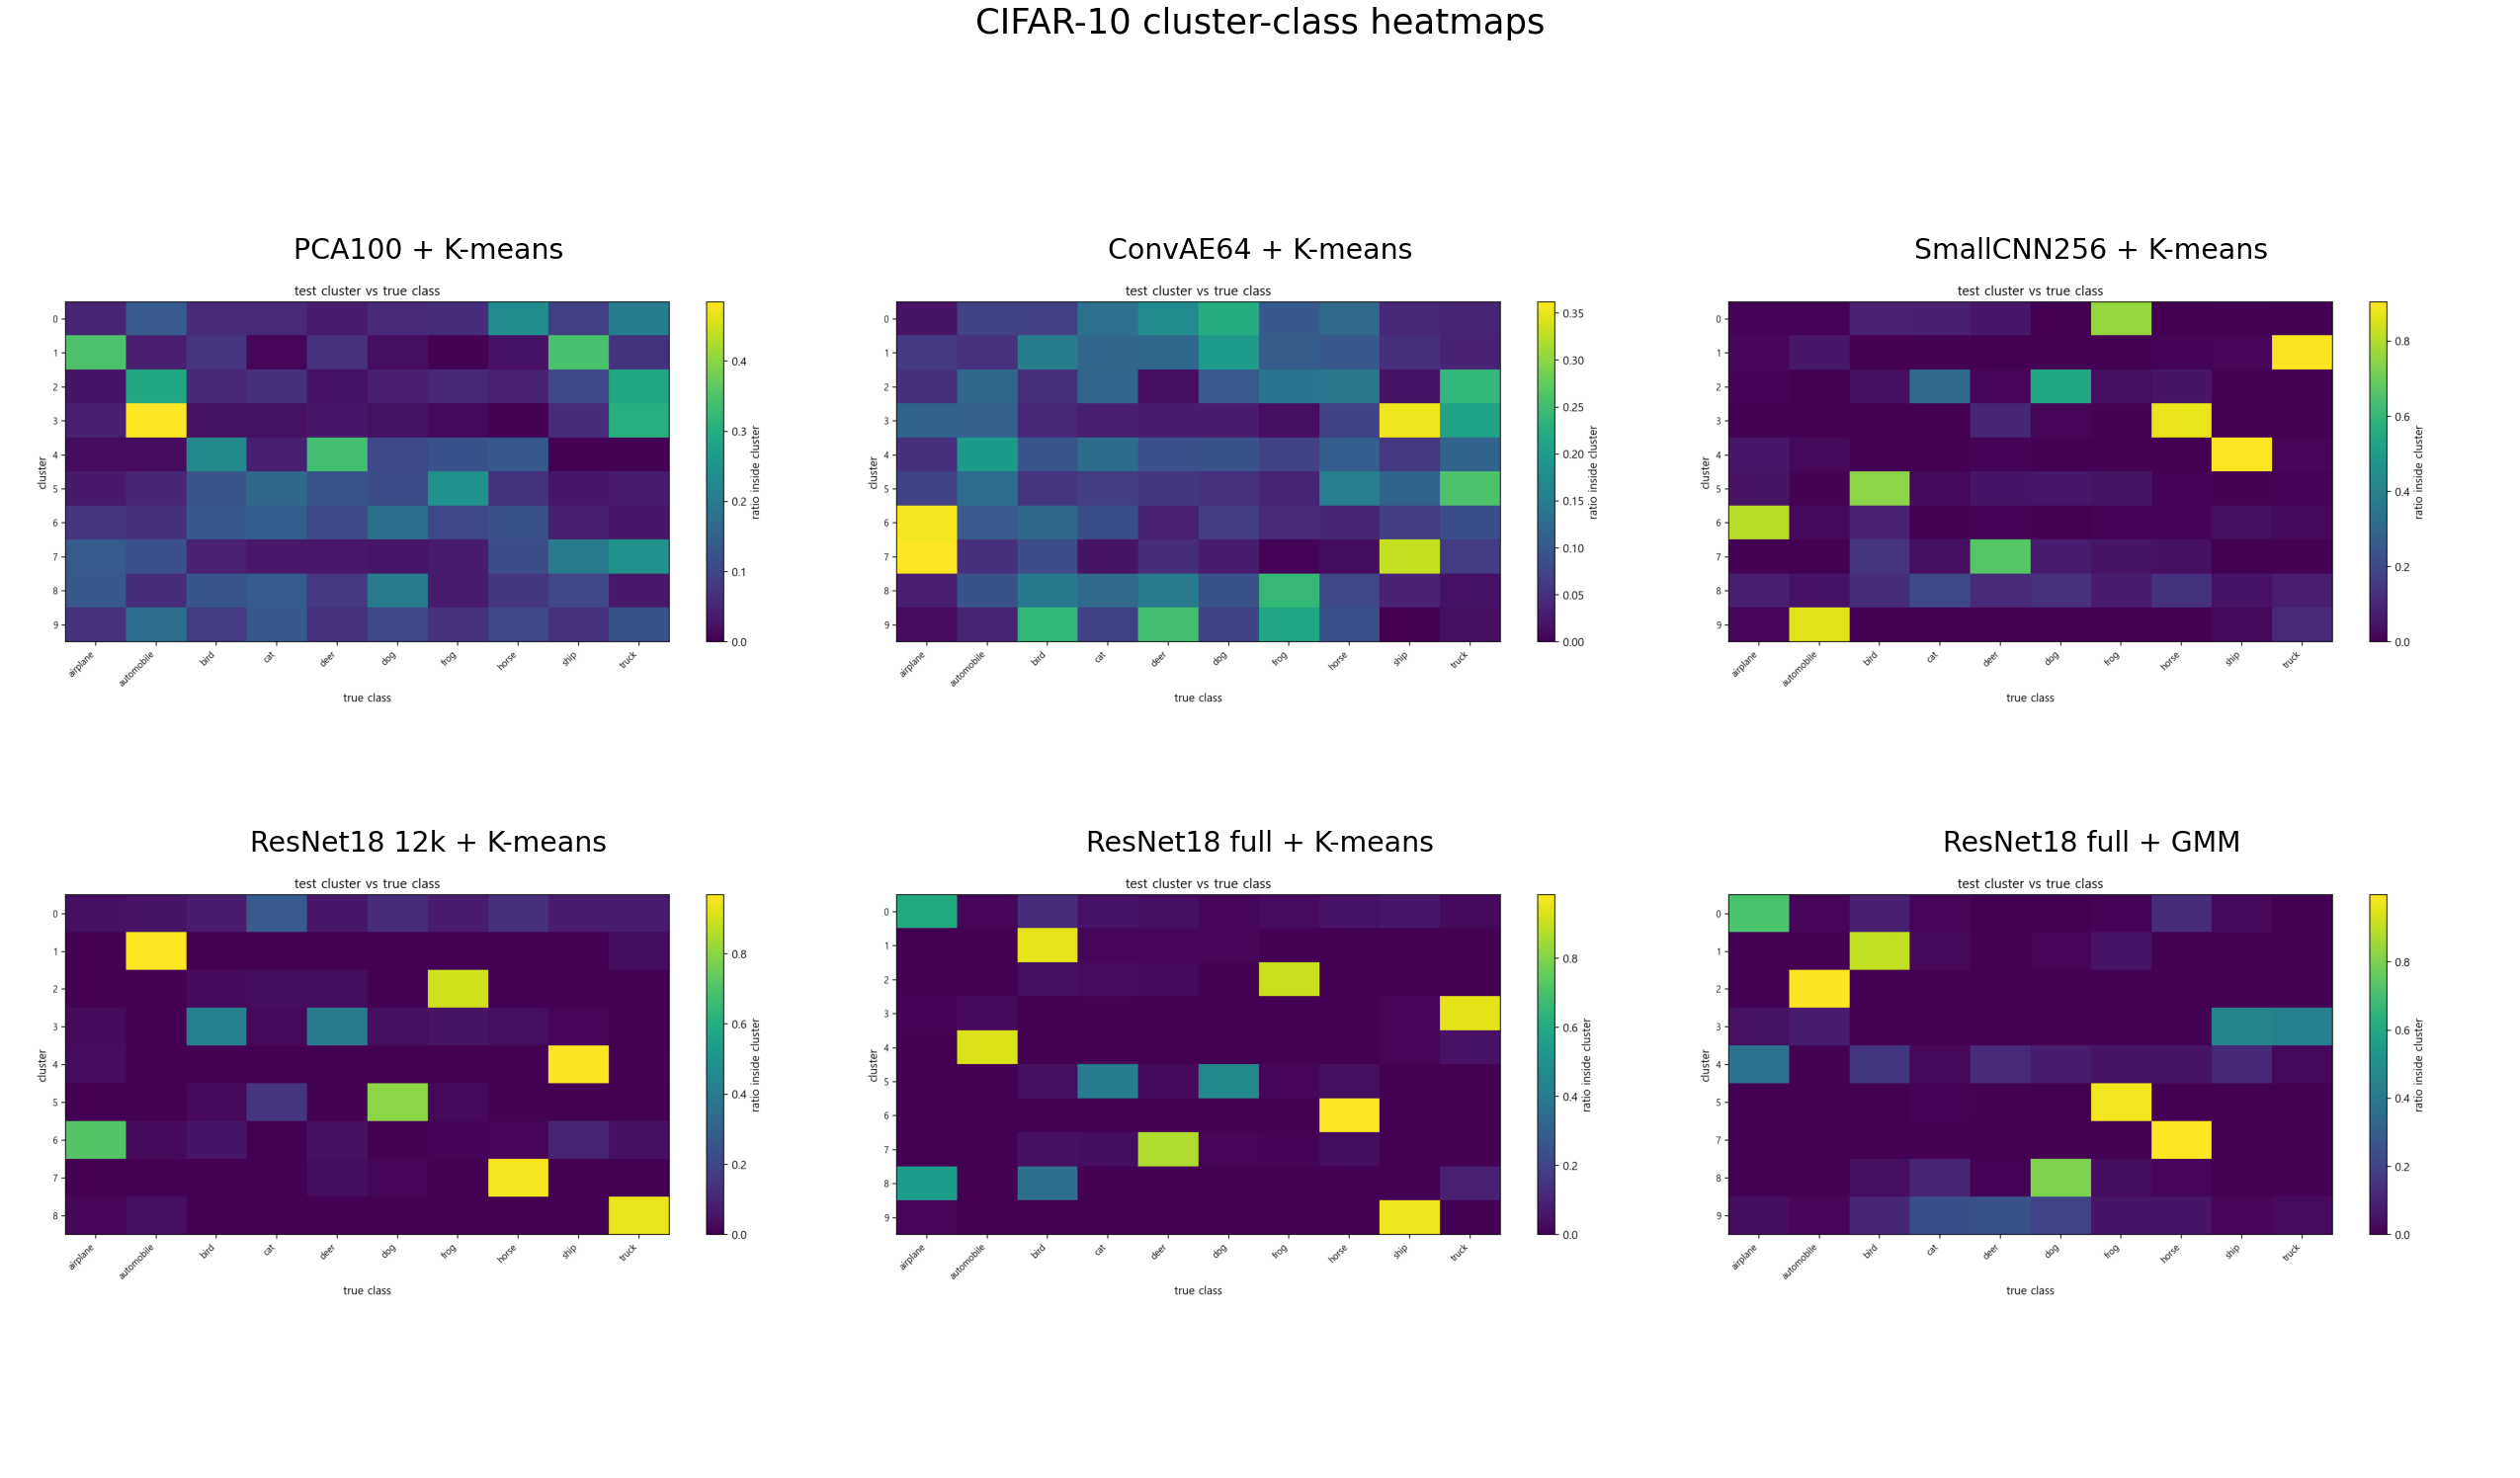
\includegraphics[width=\linewidth]{cifar10_all_runs_heatmaps.png}
    \caption{CIFAR-10 cluster-class heatmaps for selected CIFAR-10 runs. ResNet18 full + K-means gives the strongest class concentration, while GMM creates large mixed components.}
    \label{fig:cifar-all-heatmaps}
\end{figure}

Figure~\ref{fig:cifar-all-tsne}와 Figure~\ref{fig:cifar-all-heatmaps}는 같은 실험 흐름을 시각적으로 보여준다.
PCA/AE 는 t-SNE 에서 색이 넓게 섞이고 heatmap 도 여러 class 열에 퍼진다.
SmallCNN256 부터는 island 가 생기지만 중앙부 overlap 이 남는다.
ResNet18 12k 는 더 분리된 island 를 만들지만, full train split 을 사용한 ResNet18 + K-means 에서 class concentration 이 가장 뚜렷하다.
반면 ResNet18 full + GMM 은 일부 island 를 하나의 큰 색으로 덮어, clustering method 선택이 최종 결과를 크게 바꿀 수 있음을 보여준다.

\subsection{Final Model Visual Analysis}

Figure~\ref{fig:cifar-tsne}는 CIFAR-10 ResNet18 + K-means full split 의 t-SNE visualization 이다.
KMNIST 보다 class overlap 이 더 크지만, airplane, automobile, ship, truck 같은 man-made object 는 비교적 뚜렷한 group 을 형성한다.
반면 bird, cat, deer, dog, horse 같은 동물 class 들은 서로 가까운 영역에 분포하여 더 자주 섞였다.

\begin{figure}[H]
    \centering
    \begin{subfigure}{0.48\linewidth}
        \centering
        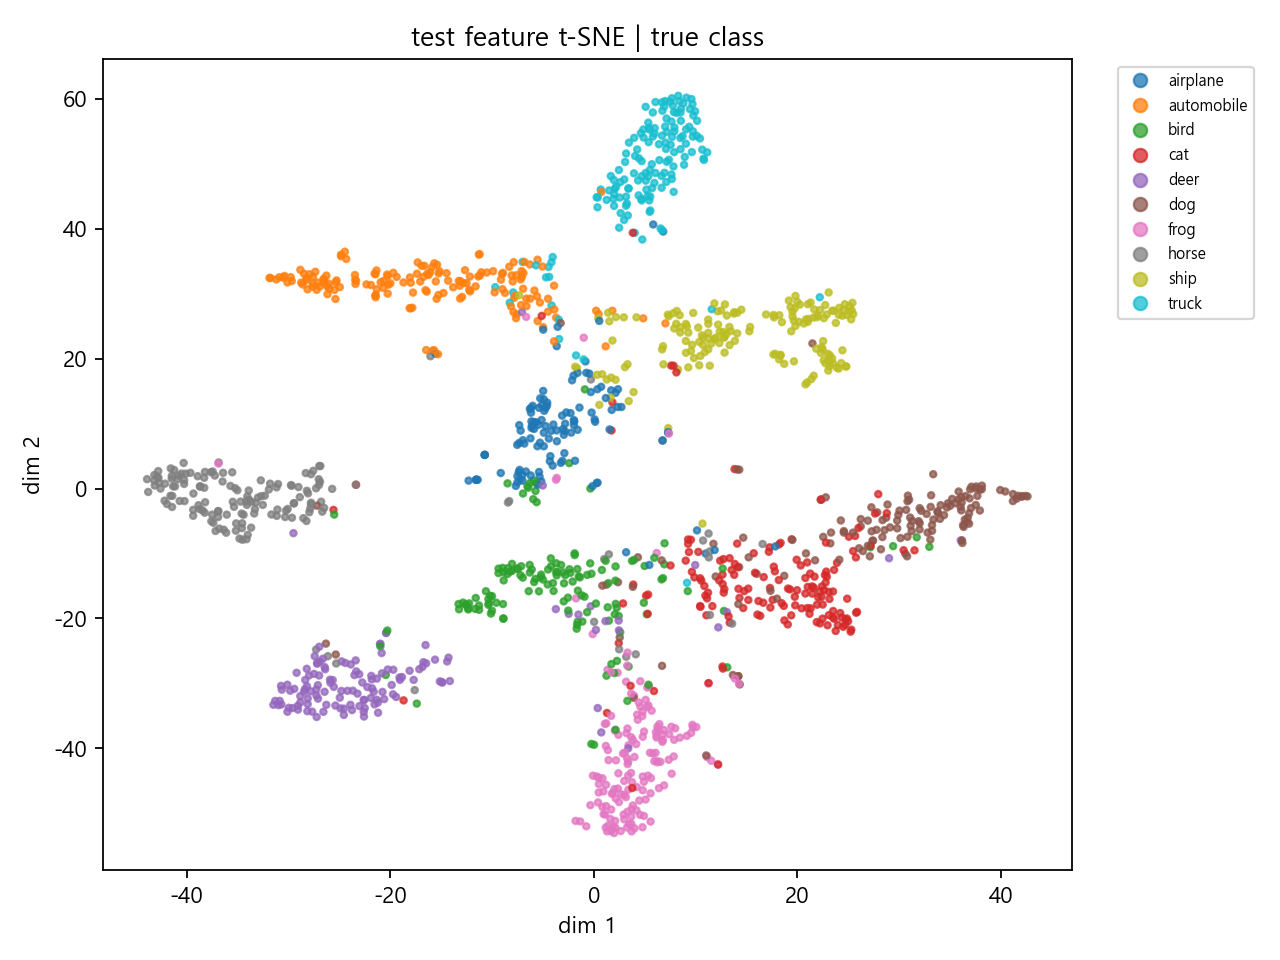
\includegraphics[width=\linewidth]{cifar10_resnet_kmeans_tsne_true.png}
        \caption{True class}
    \end{subfigure}
    \begin{subfigure}{0.48\linewidth}
        \centering
        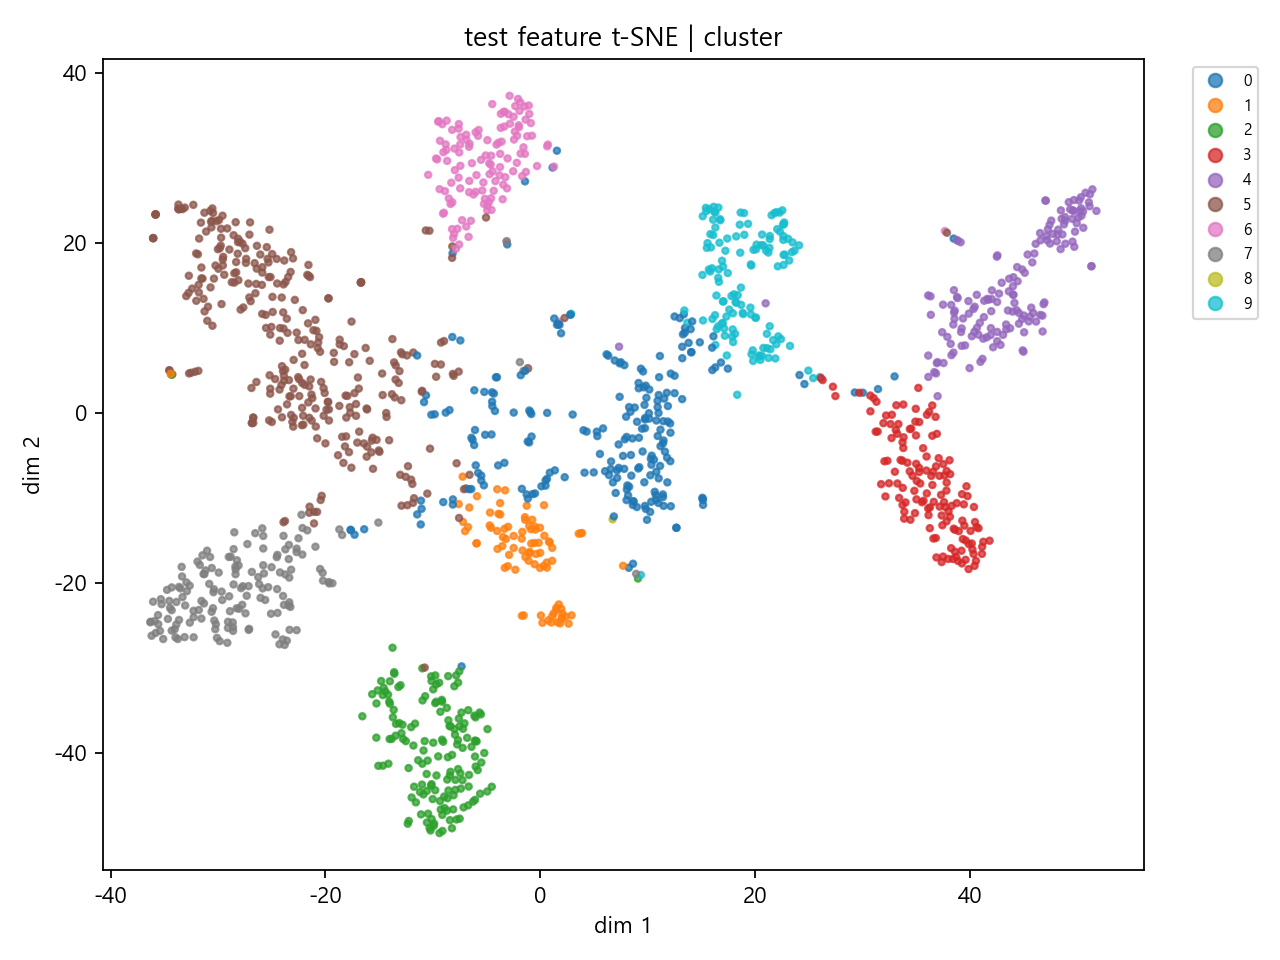
\includegraphics[width=\linewidth]{cifar10_resnet_kmeans_tsne_cluster.png}
        \caption{K-means cluster}
    \end{subfigure}
    \caption{CIFAR-10 ResNet18 + K-means t-SNE visualization on the test set.}
    \label{fig:cifar-tsne}
\end{figure}

Figure~\ref{fig:cifar-heatmap}은 K-means 와 GMM 의 cluster-class heatmap 이다.
K-means 는 상대적으로 class 별 대응이 유지되지만, GMM 은 큰 component 가 여러 class 를 흡수하여 cluster imbalance 가 심해진다.
이 때문에 GMM 은 NMI 0.5578 로 어느 정도 class 정보를 남기지만, ARI 와 purity 는 크게 낮아졌다.

\begin{figure}[H]
    \centering
    \begin{subfigure}{0.48\linewidth}
        \centering
        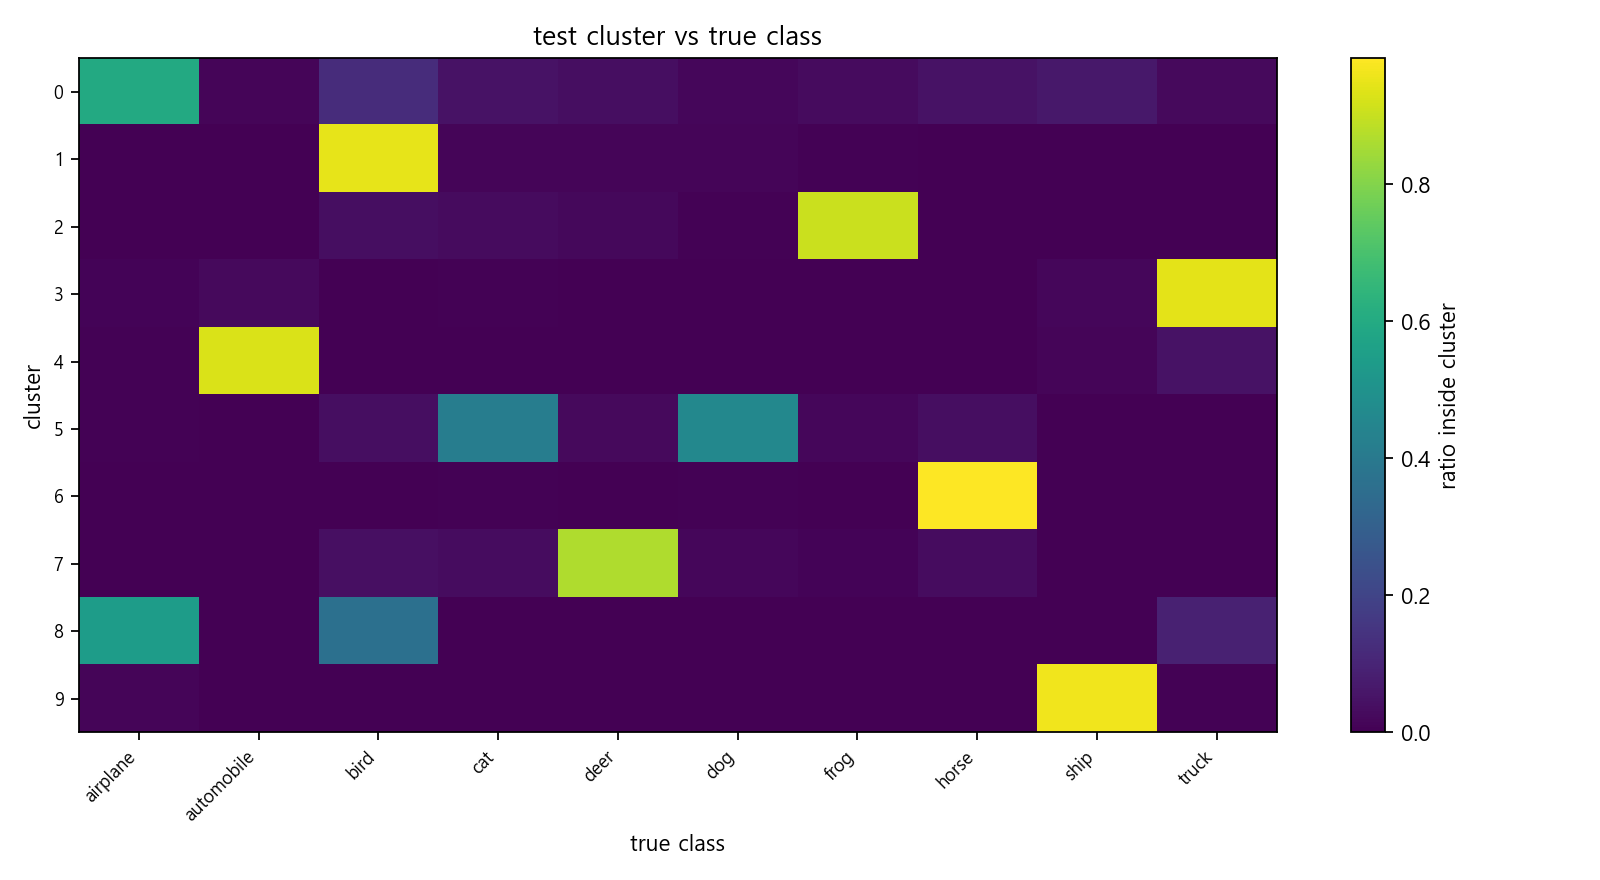
\includegraphics[width=\linewidth]{cifar10_resnet_kmeans_heatmap.png}
        \caption{K-means}
    \end{subfigure}
    \begin{subfigure}{0.48\linewidth}
        \centering
        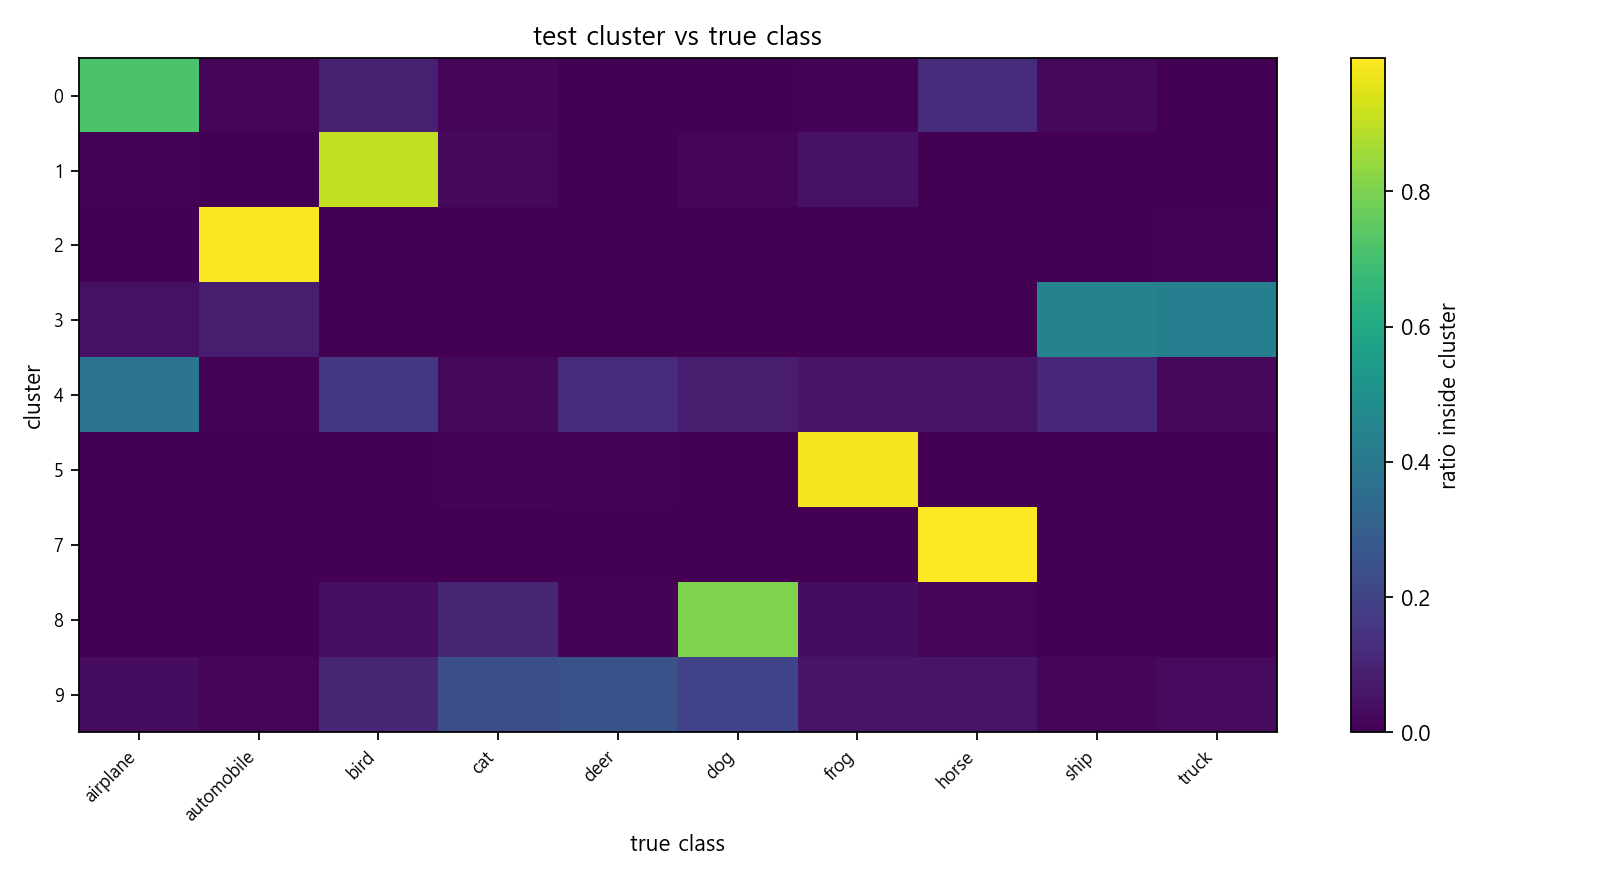
\includegraphics[width=\linewidth]{cifar10_resnet_gmm_heatmap.png}
        \caption{GMM}
    \end{subfigure}
    \caption{CIFAR-10 cluster-class relationship for ResNet18 full-split features.}
    \label{fig:cifar-heatmap}
\end{figure}

\begin{table}[H]
    \centering
    \caption{Most frequent CIFAR-10 mapped-class mismatch pairs on the test set.}
    \label{tab:cifar-mismatch-pairs}
    \begin{tabular}{llc}
        \toprule
        Run & True \(\rightarrow\) mapped class & Count\\
        \midrule
        ResNet18 + K-means full & cat \(\rightarrow\) dog & 842\\
        ResNet18 + K-means full & bird \(\rightarrow\) airplane & 204\\
        ResNet18 + K-means full & ship \(\rightarrow\) airplane & 101\\
        ResNet18 + K-means full & bird \(\rightarrow\) dog & 76\\
        ResNet18 + K-means full & cat \(\rightarrow\) airplane & 75\\
        \midrule
        ResNet18 + GMM full & cat \(\rightarrow\) deer & 929\\
        ResNet18 + GMM full & truck \(\rightarrow\) ship & 869\\
        ResNet18 + GMM full & dog \(\rightarrow\) deer & 768\\
        ResNet18 + GMM full & bird \(\rightarrow\) deer & 409\\
        ResNet18 + GMM full & frog \(\rightarrow\) deer & 221\\
        \bottomrule
    \end{tabular}
\end{table}

Table~\ref{tab:cifar-mismatch-pairs}에서 K-means 의 가장 큰 오인은 cat \(\rightarrow\) dog 이다.
Dog cluster 안에 cat sample 이 많이 들어간 것은 두 class 가 fur texture, face shape, indoor/background pattern 을 공유하기 때문이다.
Bird \(\rightarrow\) airplane 과 ship \(\rightarrow\) airplane 은 object 자체가 비슷하다기보다, 작은 object 와 넓은 배경, 수평적인 edge 가 feature space 에서 가까워진 경우로 볼 수 있다.
GMM 의 경우는 오인이 더 구조적이다.
Cat, deer, dog, bird 가 deer 쪽 component 로 크게 흡수되고, truck 이 ship component 로 들어가면서 K-means 보다 훨씬 큰 mixed component 를 만들었다.

Figure~\ref{fig:cifar-mismatch}는 CIFAR-10 에서 잘못 mapping 된 sample 들이다.
자연 이미지에서는 배경, pose, texture, object shape 이 다양하고, 동물 class 간 시각적 유사성이 크기 때문에 KMNIST 보다 semantic cluster 를 만들기 어렵다.

\begin{figure}[H]
    \centering
    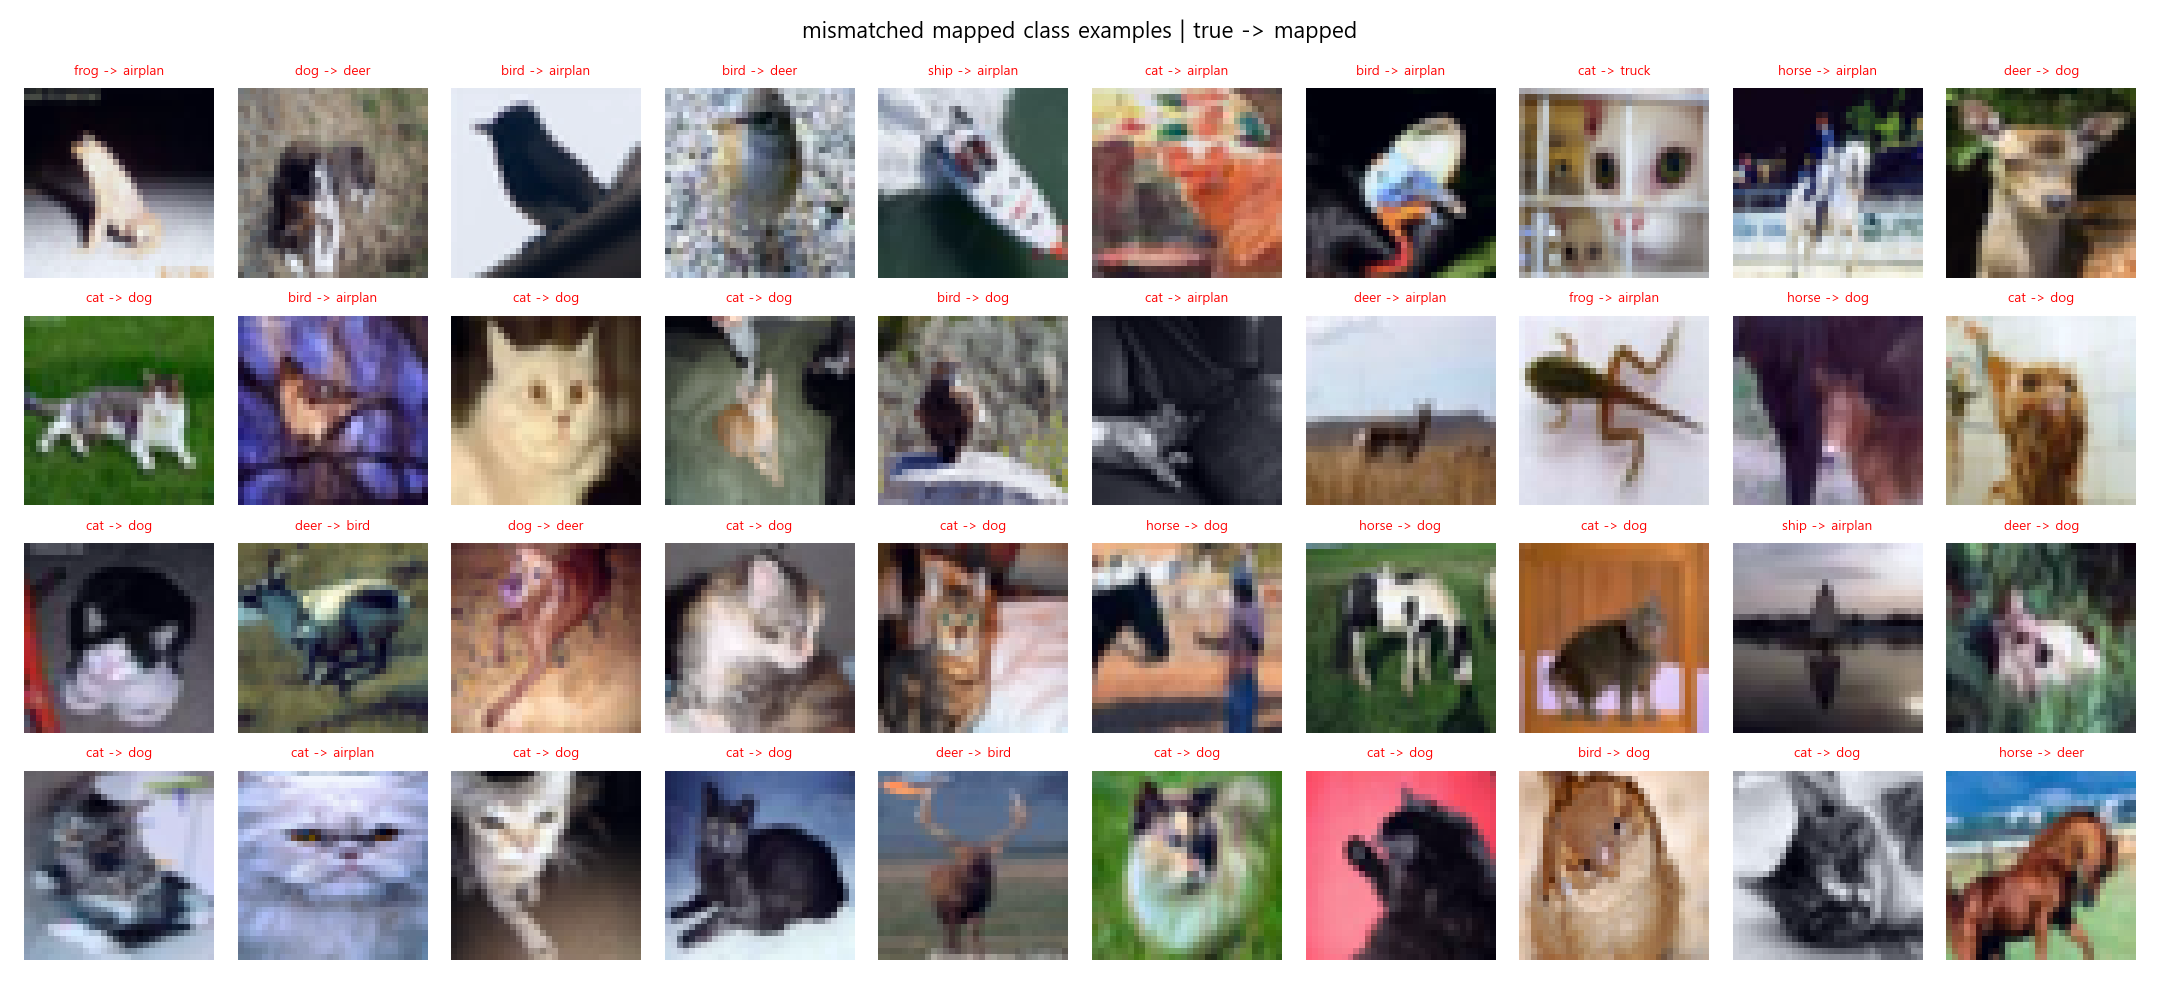
\includegraphics[width=0.86\linewidth]{cifar10_resnet_kmeans_mismatches.png}
    \caption{CIFAR-10 examples whose true class and mapped cluster class differ.}
    \label{fig:cifar-mismatch}
\end{figure}

\section{Optional Extension: DINOv2 Feature on CIFAR-10}

Required experiments 를 마친 뒤, CIFAR-10 에 대해 DINOv2 feature 를 optional extension 으로 적용하였다.
DINOv2 는 DINOv2: Learning Robust Visual Features without Supervision 논문에서 제안된 self-supervised visual feature model 이다.
본 실험에서는 DINOv2 ViT-S/14 pretrained weight 를 fine-tuning 하지 않고 고정한 상태로 사용하였다.
즉 CIFAR-10 train label 로 DINOv2 를 다시 학습하지 않았고, image embedding 만 추출한 뒤 K-means 를 적용하였다.

\subsection{DINOv2 Structure}

DINOv2 의 backbone 은 Vision Transformer(ViT)이다.
CNN 이 convolution filter 를 이미지 위에서 이동시키며 local feature map 을 만드는 것과 달리, ViT 는 이미지를 작은 patch sequence 로 바꾼 뒤 Transformer block 으로 token 사이의 관계를 계산한다.
본 실험에서 사용한 ViT-S/14 는 입력 이미지를 \(224\times224\)로 resize 하고, 이를 \(14\times14\) 크기의 patch 로 나눈다.
따라서 한 이미지는 \(16\times16=256\)개의 patch token 으로 표현된다.
여기에 image 전체를 대표하는 class token 이 추가되고, token 들은 여러 Transformer self-attention block 을 통과한다.
최종 class token 또는 image-level output 은 이미지 전체의 semantic representation 으로 볼 수 있으며, 본 실험에서는 이 vector 를 clustering feature 로 사용하였다.

\begin{figure}[H]
    \centering
    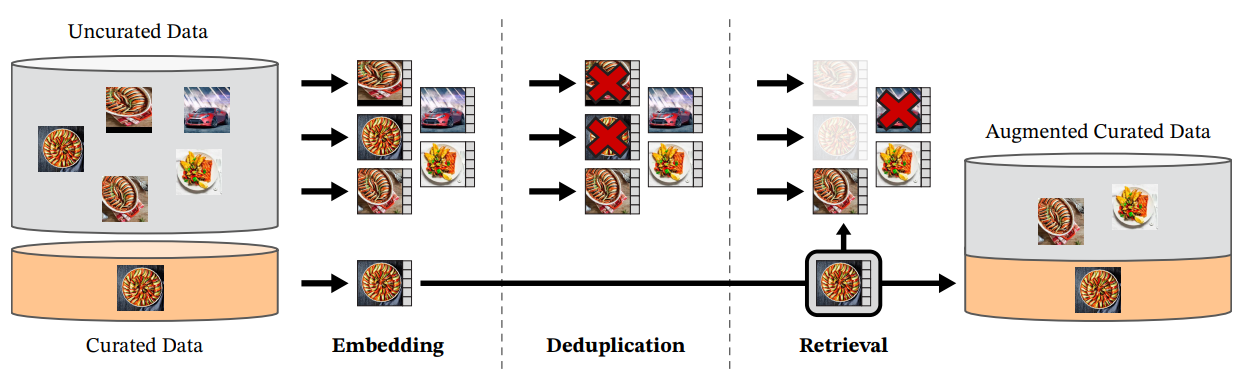
\includegraphics[width=0.86\linewidth]{dinov2_structure_img.png}
    \caption{DINOv2 structure. The model converts an image into patch tokens, processes them with a Vision Transformer, and produces an image-level feature representation.}
    \label{fig:dinov2-structure}
\end{figure}

DINOv2 의 핵심은 이 ViT backbone 을 human label 없이 학습한다는 점이다.
일반 supervised CNN 은 image 와 class label 을 함께 보고 cross-entropy loss 로 학습한다.
반면 DINO 계열 방법은 같은 image 에서 만들어진 서로 다른 augmented view 를 보고, 서로 일관된 representation 을 만들도록 학습한다.
개념적으로는 teacher network 가 만든 target representation 을 student network 가 따라가도록 만드는 self-distillation 구조이다.
이 과정에서 class label 은 사용하지 않지만, 충분히 다양한 이미지로 학습하면 object shape, texture, part relation 과 같은 시각적 구조가 embedding 안에 남는다.
DINOv2 는 이런 self-supervised ViT feature 를 대규모 curated image data 에서 학습하여, fine-tuning 없이도 여러 vision task 에 사용할 수 있는 general-purpose feature 를 목표로 한다.

\subsection{Experimental Use}

CIFAR-10 이미지는 원래 \(32\times32\) RGB image 이지만, DINOv2 입력 크기에 맞추어 \(224\times224\)로 resize 하였다.
그 뒤 pretrained DINOv2 ViT-S/14 에 넣어 384차원 image embedding 을 얻었다.
이 embedding 은 StandardScaler 로 scaling 한 뒤, 기존 실험과 같은 K-means \(k=10\)에 넣었다.
Train split 은 K-means center 를 fit 하는 데만 사용하고, test split 은 학습된 K-means model 로 cluster 를 예측하였다.
Label 은 clustering model 학습에는 사용하지 않고, ARI/NMI/purity 계산에서만 사용하였다.

DINOv2 는 CIFAR-10 에만 적용하였다.
CIFAR-10 은 자연 이미지 데이터셋이므로 대규모 자연 이미지로 학습된 pretrained encoder 와 domain 이 비교적 잘 맞는다.
반면 KMNIST 는 손글씨 문자 이미지라서, 자연 이미지 foundation feature 를 바로 적용했을 때의 해석이 CIFAR-10 보다 덜 직접적이다.

\begin{table}[H]
    \centering
    \caption{Optional DINOv2 feature result on CIFAR-10 test split. All rows use K-means with \(k=10\).}
    \label{tab:cifar-foundation-results}
    \begin{tabular}{lcccc}
        \toprule
        Feature & ARI & NMI & Purity & Silhouette\\
        \midrule
        ResNet18 supervised full & 0.6408 & 0.7252 & 0.7825 & 0.2747\\
        DINOv2 ViT-S/14 & \textbf{0.7969} & \textbf{0.8414} & \textbf{0.9053} & 0.0789\\
        \bottomrule
    \end{tabular}
\end{table}

Table~\ref{tab:cifar-foundation-results}와 Figure~\ref{fig:cifar-foundation-metrics}를 보면, DINOv2 feature 가 ARI, NMI, purity 에서 가장 높다.
ResNet18 full run 은 CIFAR-10 label 로 20 epochs 학습한 feature 인데도, DINOv2 frozen feature 보다 낮았다.
이는 대규모 image pretraining 으로 얻은 representation 이 CIFAR-10 의 object-level structure 를 더 잘 보존할 수 있음을 보여준다.

\begin{figure}[H]
    \centering
    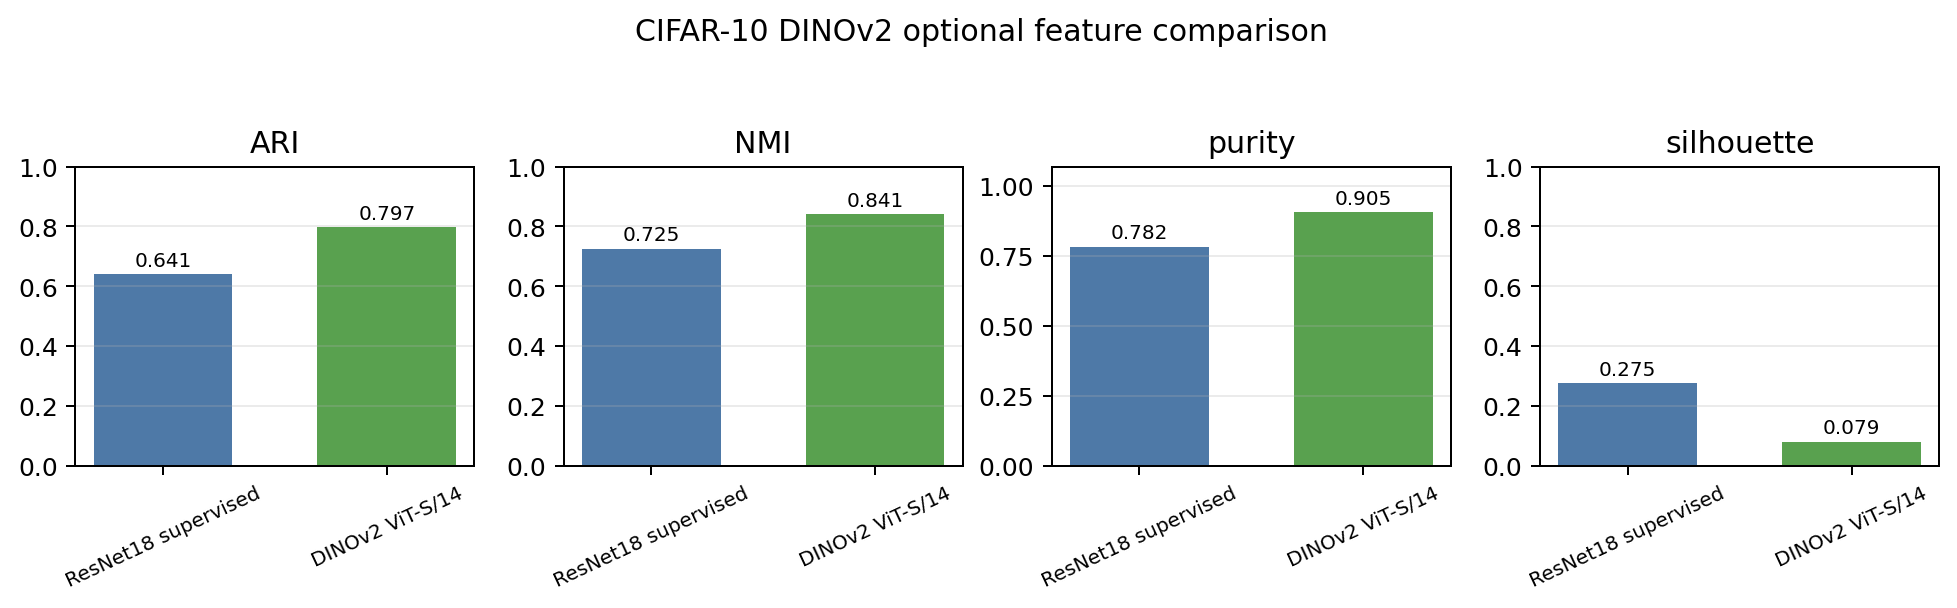
\includegraphics[width=\linewidth]{cifar10_optional_foundation_metrics.png}
    \caption{CIFAR-10 optional DINOv2 feature comparison. DINOv2 improves label-based clustering metrics over the supervised ResNet18 full run.}
    \label{fig:cifar-foundation-metrics}
\end{figure}

Silhouette 은 반대로 ResNet18 이 더 높았다.
이 결과는 ARI/NMI/purity 와 다른 방향이다.
Silhouette 은 label 을 보지 않고 feature space 의 geometric compactness 만 측정한다.
DINOv2 feature 는 class 정보를 더 많이 보존하지만, K-means cluster 가 Euclidean distance 기준으로 ResNet18 feature 보다 더 compact 하게 보이지는 않았다.
따라서 optional comparison 에서는 label correspondence 를 보는 ARI, NMI, purity 를 더 중요하게 해석하였다.

\begin{figure}[H]
    \centering
    \begin{subfigure}{0.49\linewidth}
        \centering
        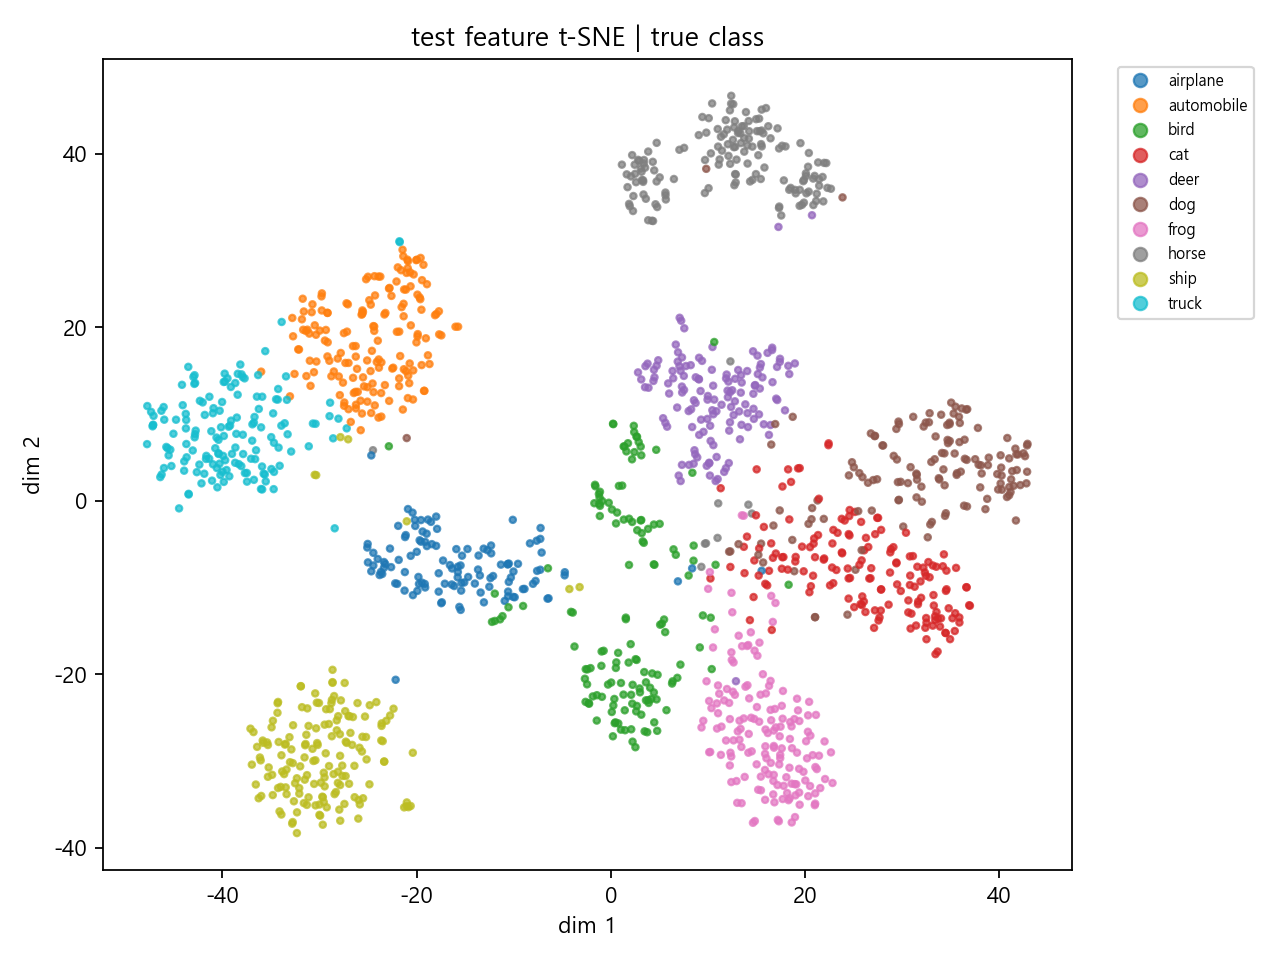
\includegraphics[width=\linewidth]{cifar10_dinov2_tsne_true.png}
        \caption{True class}
    \end{subfigure}
    \begin{subfigure}{0.49\linewidth}
        \centering
        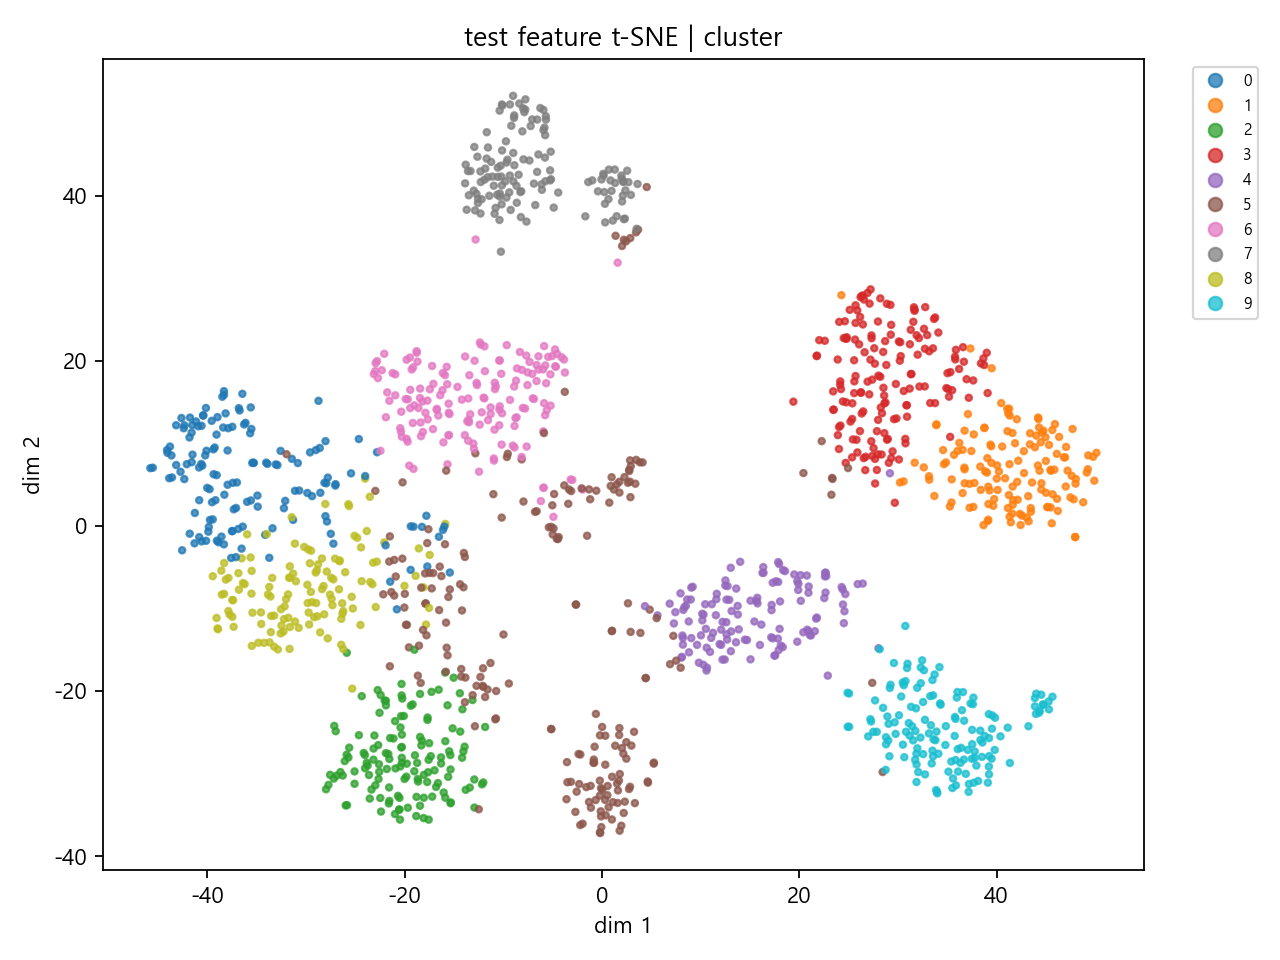
\includegraphics[width=\linewidth]{cifar10_dinov2_tsne_cluster.png}
        \caption{K-means cluster}
    \end{subfigure}
    \caption{DINOv2 feature t-SNE visualization on CIFAR-10 test split. The cluster view follows the true-class structure more clearly than PCA/AE/CNN baseline visualizations.}
    \label{fig:cifar-dinov2-tsne}
\end{figure}

Figure~\ref{fig:cifar-dinov2-tsne}에서도 DINOv2 feature 는 여러 class 를 비교적 분리된 island 로 만든다.
완전히 분리되지는 않지만, Table~\ref{tab:cifar-foundation-results}의 높은 ARI/NMI 와 같은 방향이다.

\begin{figure}[H]
    \centering
    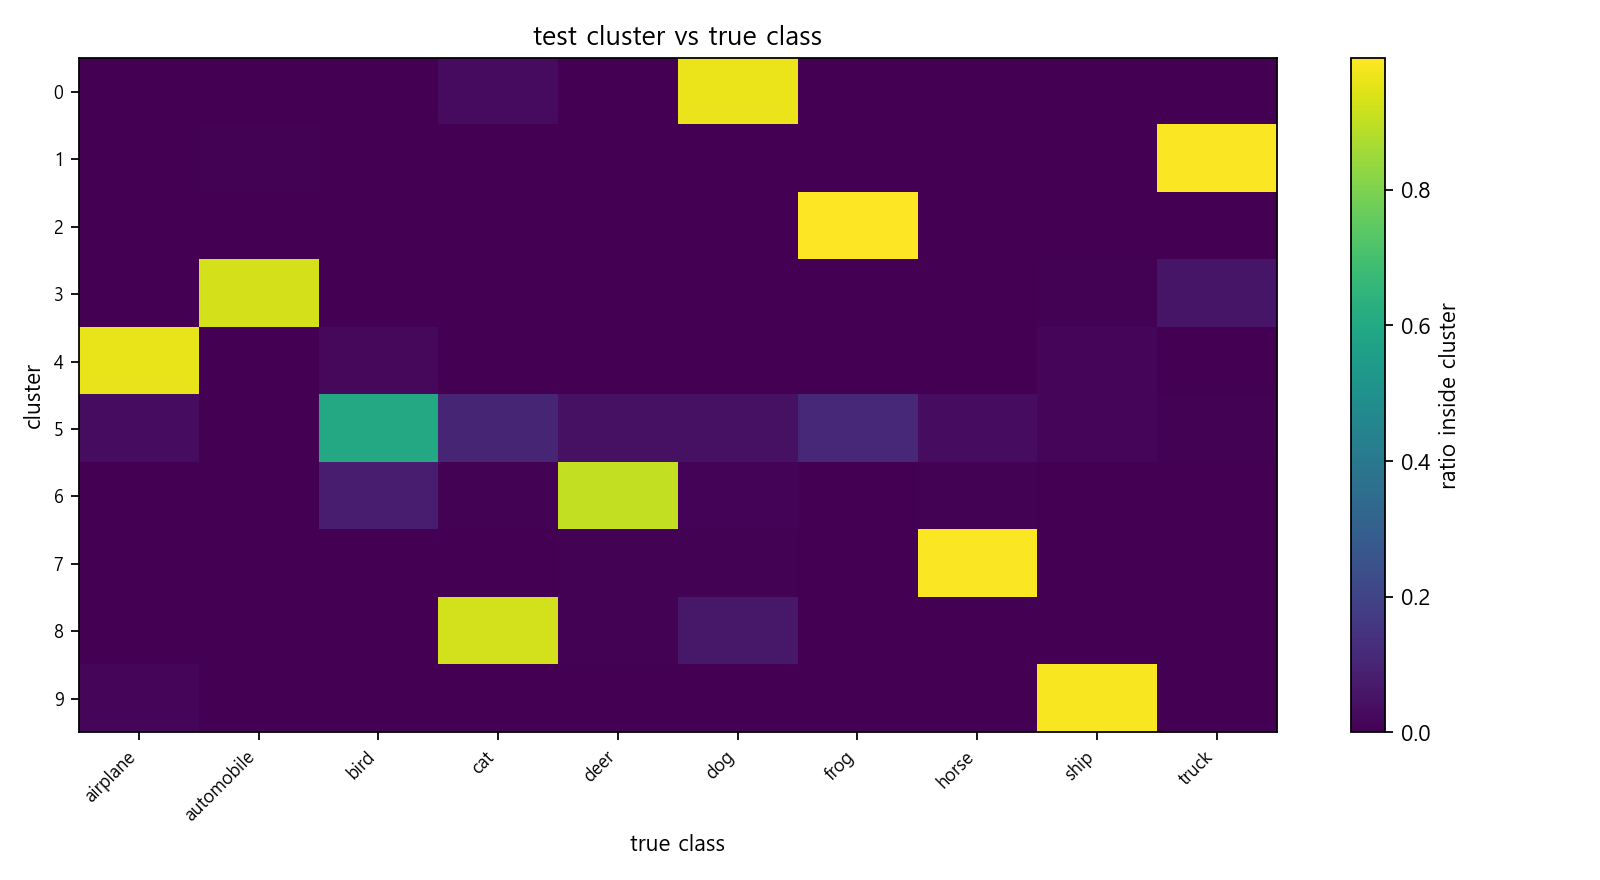
\includegraphics[width=0.72\linewidth]{cifar10_dinov2_heatmap.png}
    \caption{Cluster-class heatmap for DINOv2 feature on CIFAR-10. Several clusters have clear dominant classes, explaining the higher ARI/NMI/purity.}
    \label{fig:cifar-foundation-heatmaps}
\end{figure}

이 optional 실험의 한계도 있다.
DINOv2 는 이미 대규모 외부 데이터로 학습된 모델이므로, required component 의 PCA/AE/CNN 비교와 같은 조건은 아니다.
또한 이 실험은 frozen feature 를 바로 사용한 것이며, CIFAR-10 에 맞춘 fine-tuning, self-labeling, contrastive clustering 까지는 수행하지 않았다.
그럼에도 DINOv2 결과는 CIFAR-10 clustering 에서 feature representation 의 품질이 clustering algorithm 선택만큼 중요하다는 점을 보여준다.

\section{Cross-Dataset Discussion}

\subsection{Overall Metric Comparison}

Figure~\ref{fig:selected-metrics}는 주요 실험의 metric 을 한 번에 비교한 것이다.
Required main \(k=10\) experiments 에서는 두 데이터셋 모두 ResNet18 + K-means full split 이 가장 좋은 조합이었다.
그러나 그 의미는 조금 다르다.
KMNIST 는 SmallCNN 만으로도 ARI 0.6492 를 얻었고, ResNet18 로 구조를 바꾸면 12k subset 에서도 ARI 0.8916 까지 상승하였다.
CIFAR-10 은 SmallCNN 과 ResNet18 12k subset 의 차이가 크지 않았지만, full train set 으로 학습했을 때 ResNet18 feature 의 성능이 크게 올라갔다.
Optional extension 에서는 CIFAR-10 DINOv2 frozen feature 가 ResNet18 full run 보다 더 높은 ARI/NMI/purity 를 보였지만, 이는 대규모 외부 pretraining 을 사용한 별도 비교로 해석하였다.

\begin{figure}[H]
    \centering
    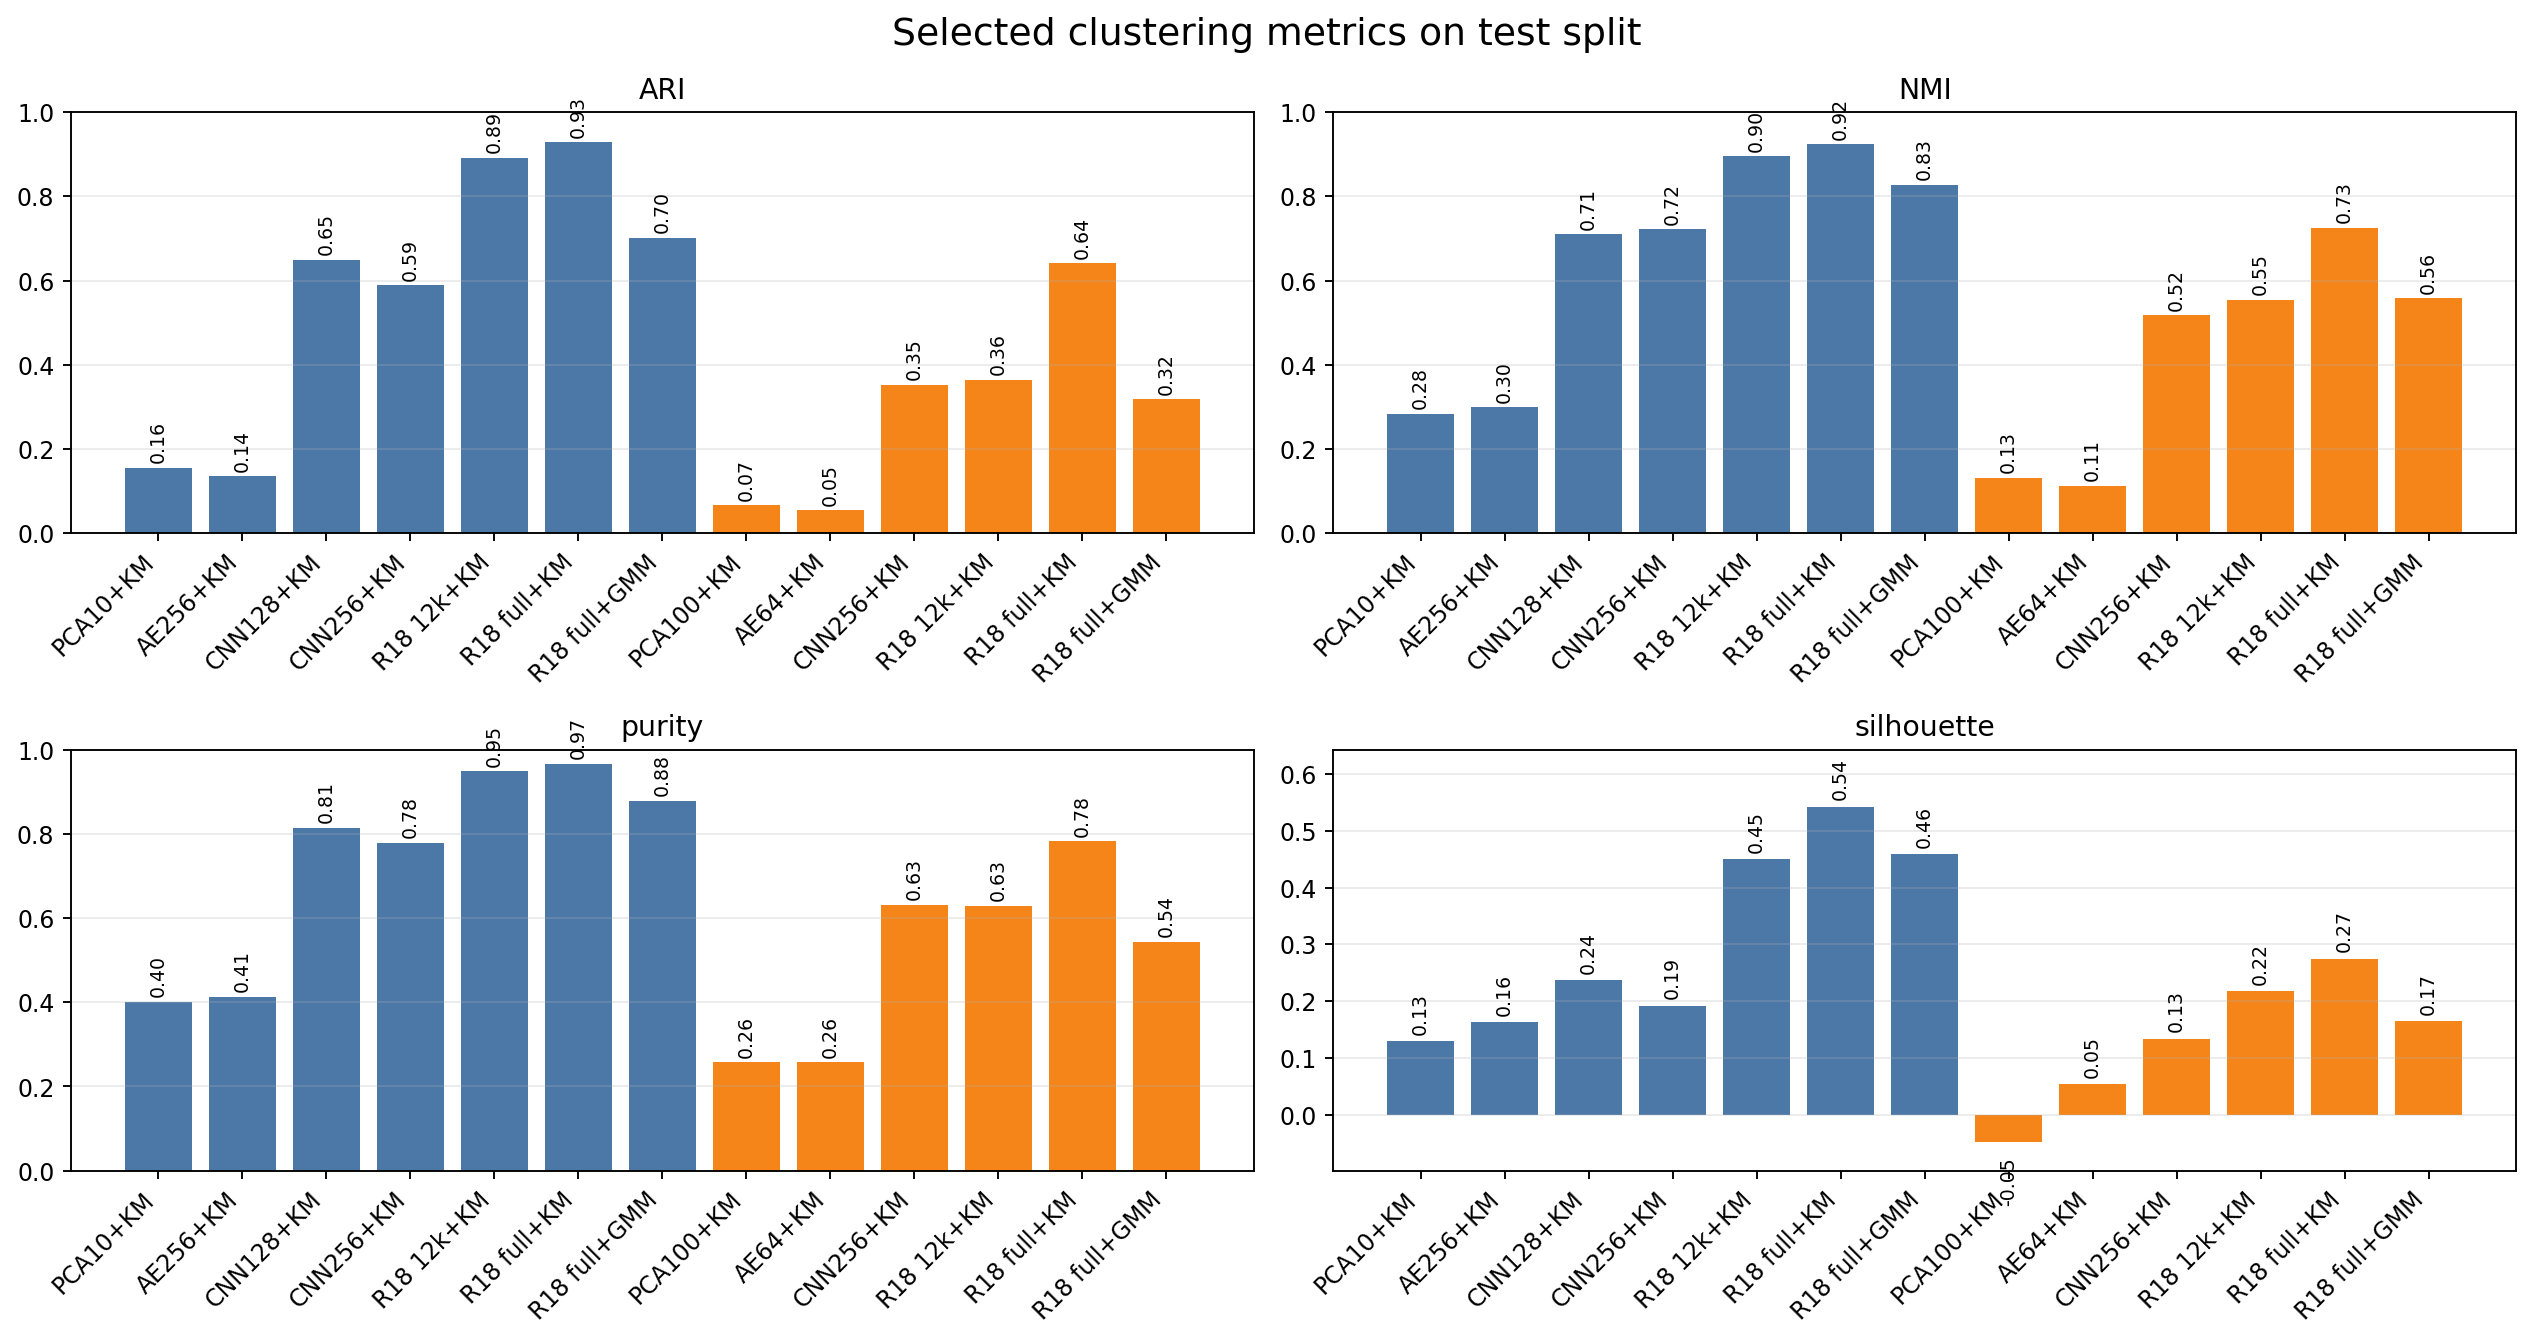
\includegraphics[width=\linewidth]{selected_metric_bars.png}
    \caption{Selected quantitative results on test split. Blue bars are KMNIST runs and orange bars are CIFAR-10 runs.}
    \label{fig:selected-metrics}
\end{figure}

PCA 와 AutoEncoder 는 두 데이터셋 모두에서 CNN 계열 feature 보다 낮았다.
PCA 는 pixel-level variance 를 보존하지만 semantic class 를 직접 분리하지 않는다.
AutoEncoder 도 reconstruction 을 잘하도록 학습되므로, latent space 가 class 별로 분리되도록 강제되지 않는다.
반면 supervised CNN feature 는 label prediction 을 위해 class-discriminative feature 를 학습하므로, K-means 가 사용할 수 있는 더 의미 있는 embedding 을 만들었다.

\subsection{Cluster Number Sensitivity}

Feature dimension 에 대한 sensitivity 는 Figure~\ref{fig:pca-component-sweep}--\ref{fig:ae-epoch-sweep}에서 feature 설정과 함께 확인하였다.
여기서는 최종 feature 인 ResNet18 full embedding 에서 K-means cluster 수 \(k\)만 바꾸었을 때의 변화를 비교한다.

\begin{figure}[H]
    \centering
    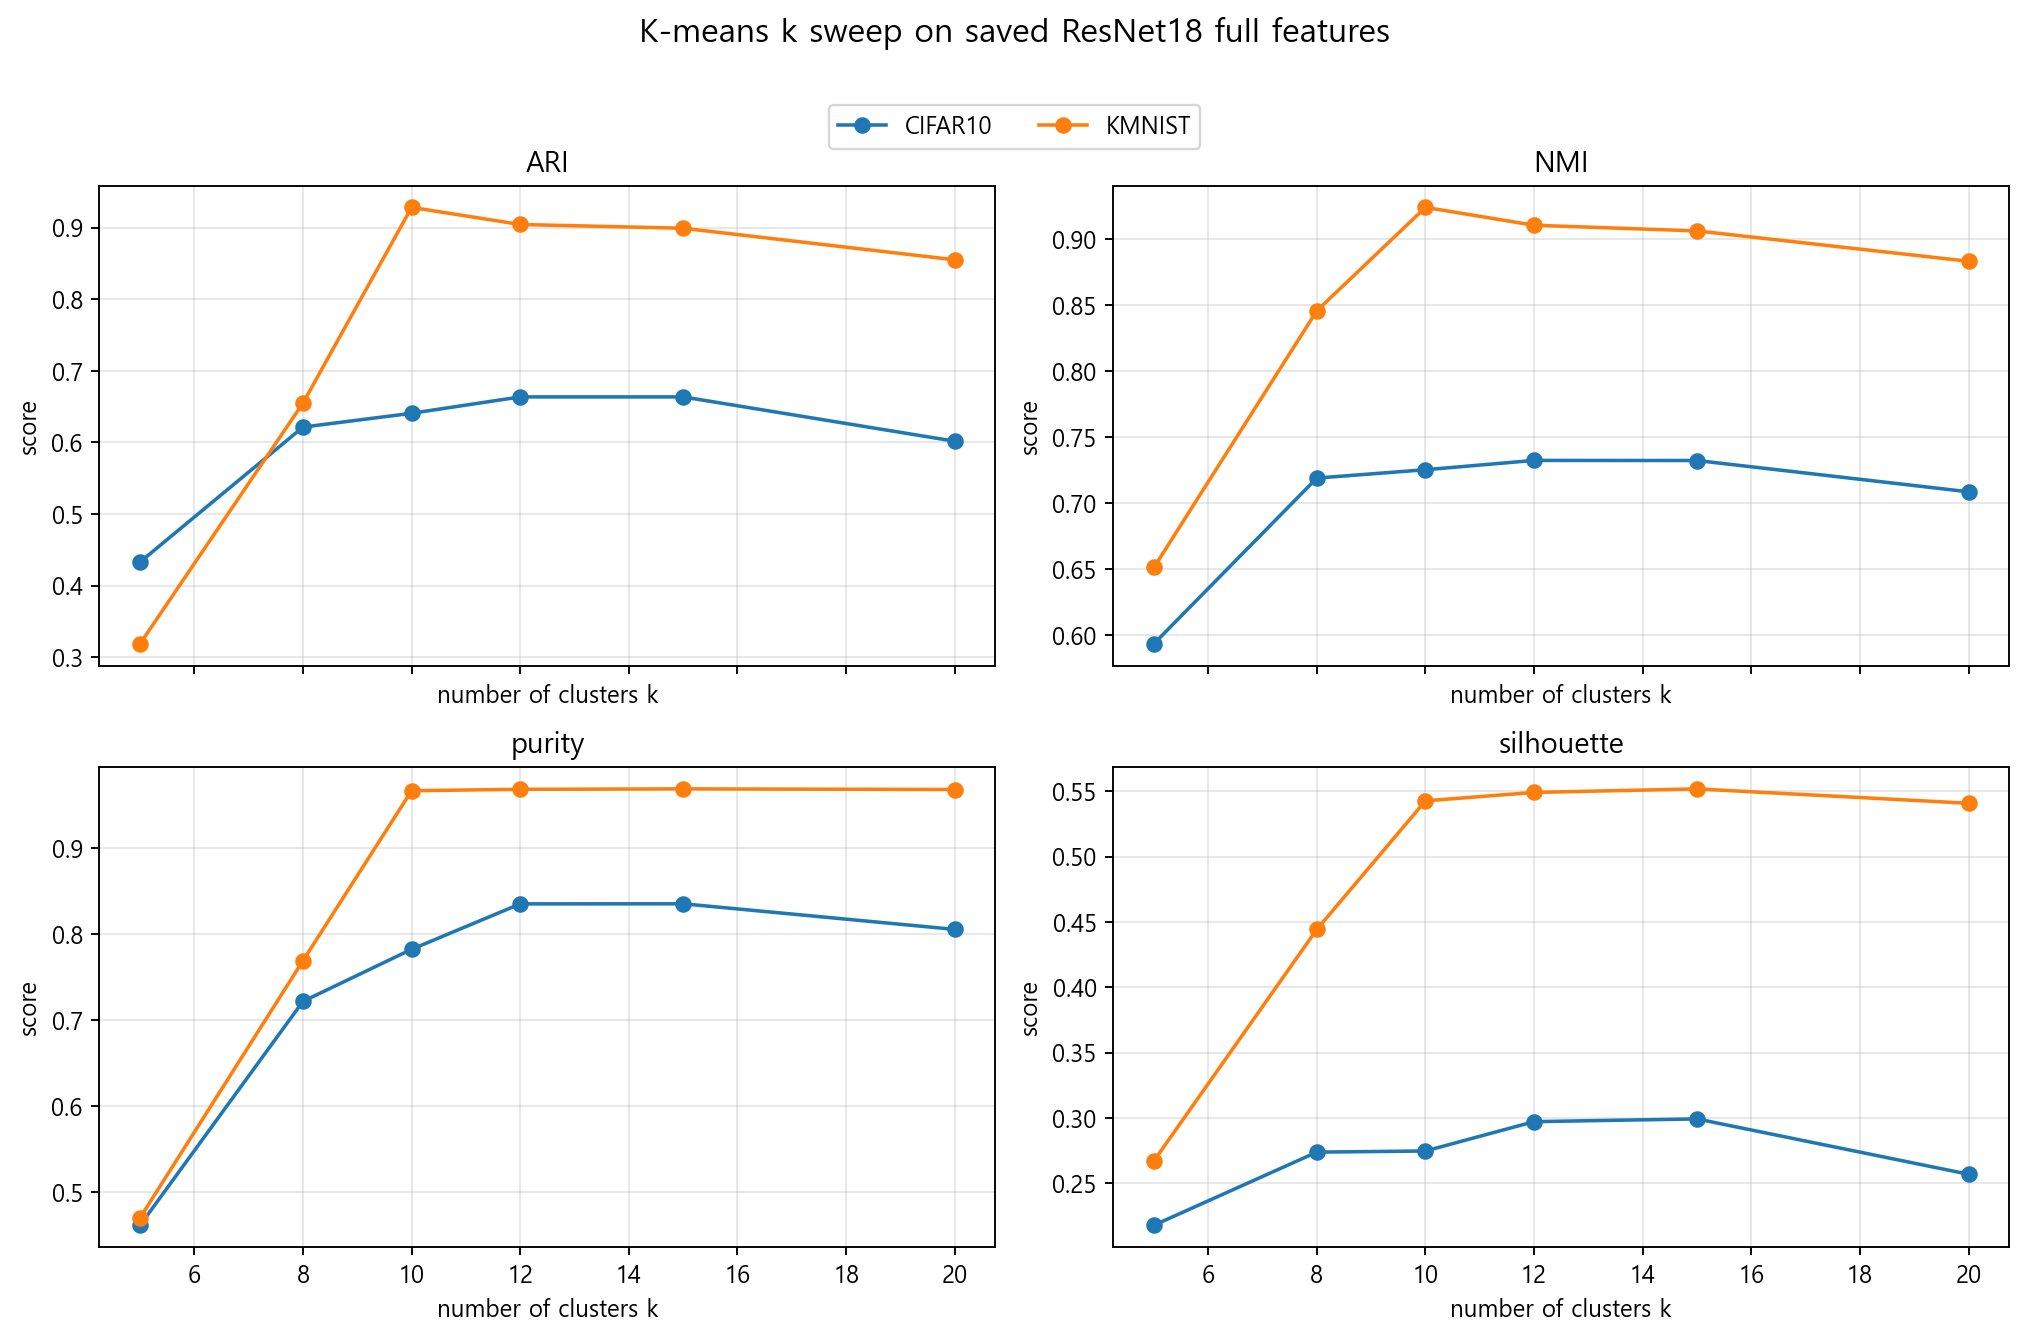
\includegraphics[width=\linewidth]{k_sweep_resnet_full_metrics.png}
    \caption{K-means \(k\) sweep on saved ResNet18 full features. The main experiments use \(k=10\) because both datasets have 10 classes.}
    \label{fig:k-sweep}
\end{figure}

Figure~\ref{fig:k-sweep}는 최종 feature 인 ResNet18 full embedding 에서 \(k\)만 바꾸어 K-means 를 다시 수행한 결과이다.
KMNIST 는 \(k=10\)에서 ARI 0.9284, NMI 0.9238 로 가장 좋았다.
\(k=12\)와 \(k=15\)에서는 purity 가 0.9688, 0.9693 으로 아주 조금 높아졌지만, ARI 와 NMI 는 낮아졌다.
Purity 는 cluster 수가 늘어나면 올라가기 쉬운 지표이므로, KMNIST 에서는 class 수와 같은 \(k=10\) 설정이 가장 설득력 있었다.

CIFAR-10 은 \(k=10\)에서 ARI 0.6408 이었고, \(k=12\)와 \(k=15\)에서 ARI 0.6637 수준까지 올라갔다.
이는 CIFAR-10 feature space 에서 일부 semantic class 가 하나의 compact cluster 로 모이기보다 여러 subtype 으로 나뉠 수 있음을 의미한다.
예를 들어 같은 class 안에서도 pose, background, object scale 이 크게 달라질 수 있다.
다만 과제의 기본 비교는 10개 class 를 기준으로 하므로, 최종 표와 주 비교에서는 \(k=10\)을 유지하였다.

\subsection{K-means vs. GMM}

본 실험에서는 GMM 이 K-means 보다 일관되게 좋지 않았다.
특히 full ResNet18 feature 에서 K-means 와 GMM 은 같은 CNN feature 를 사용했기 때문에, 차이는 feature extractor 가 아니라 clustering 단계에서 발생한 것이다.
Figure~\ref{fig:cluster-size}는 K-means 와 GMM 의 cluster size 를 비교한다.
K-means 는 cluster size 가 비교적 균형을 이루지만, GMM 은 큰 component 가 여러 class 를 흡수하는 경향을 보였다.

\begin{figure}[H]
    \centering
    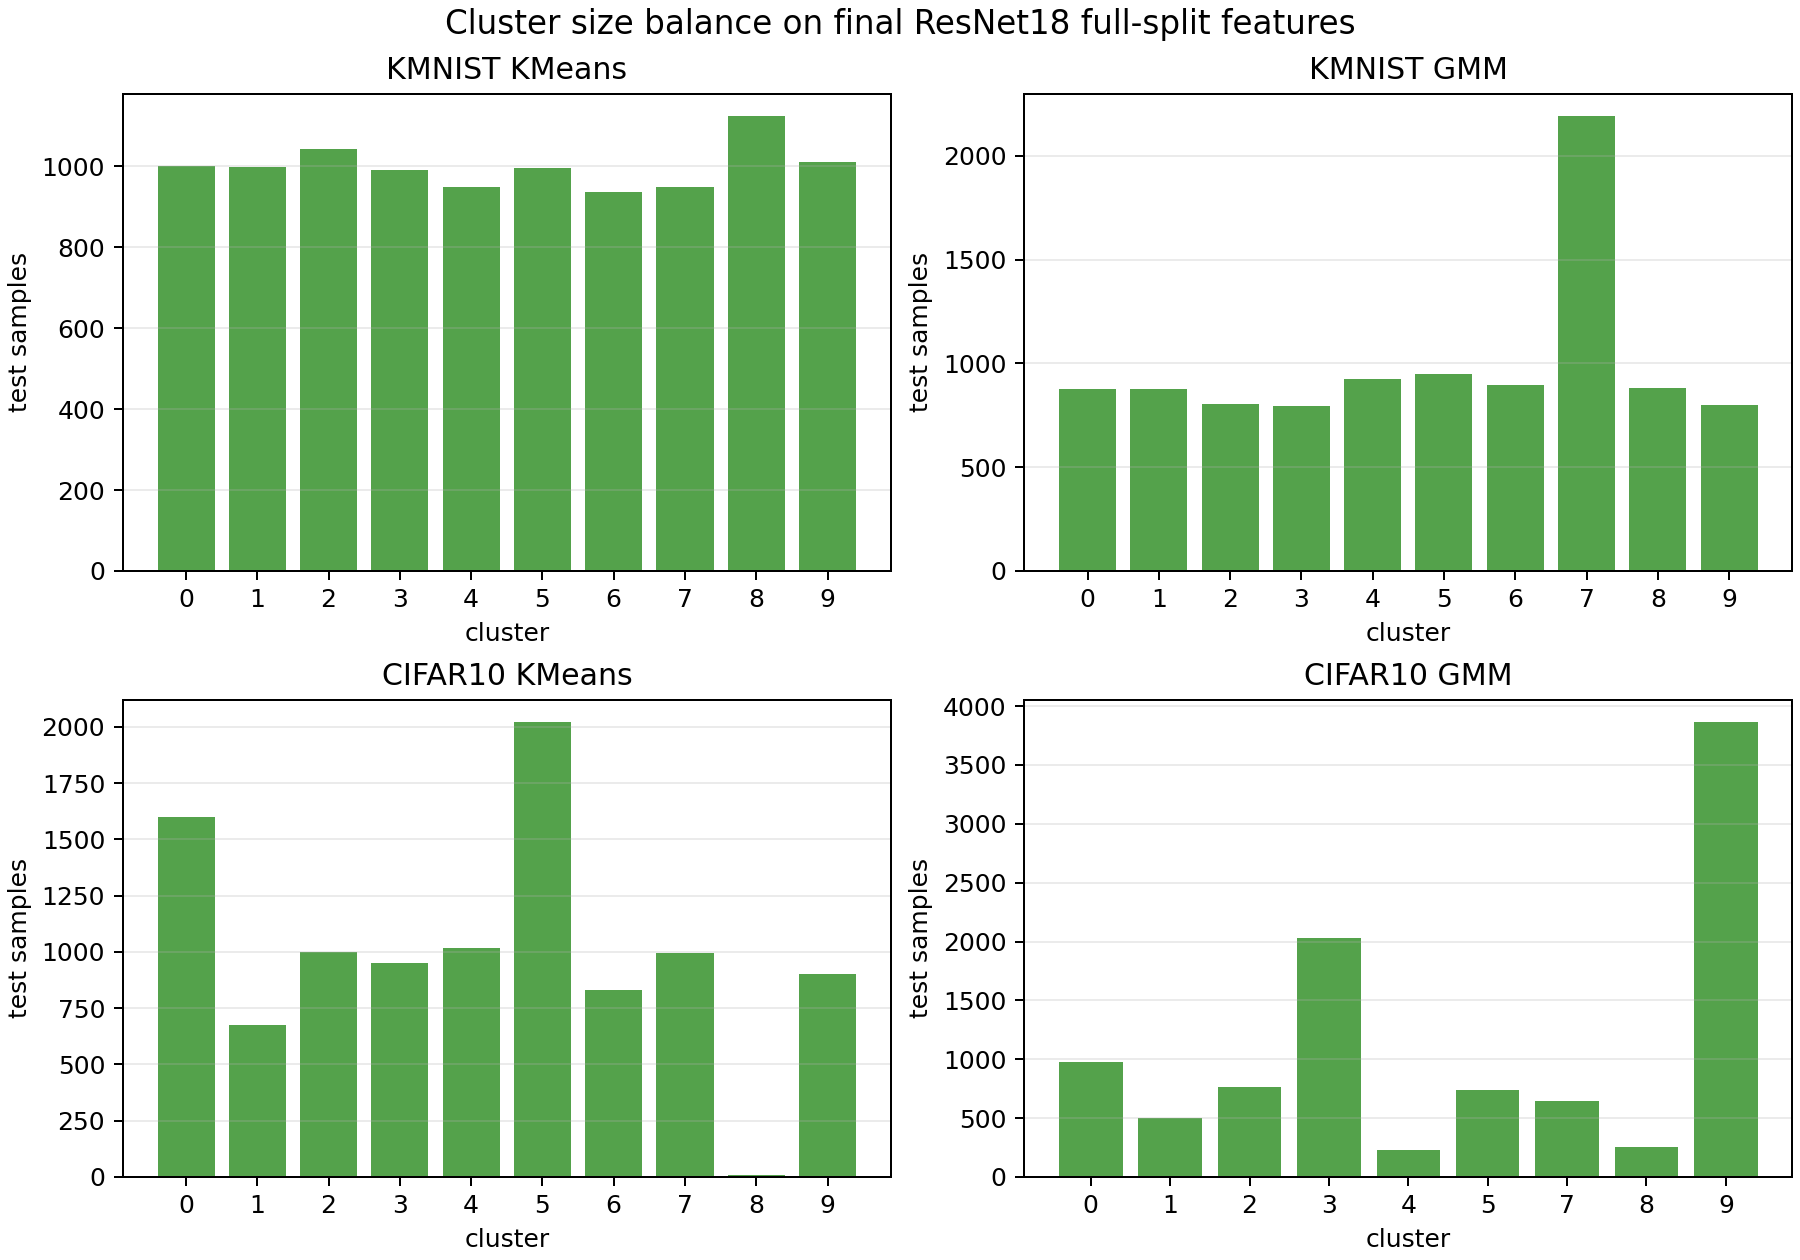
\includegraphics[width=0.88\linewidth]{resnet_full_cluster_sizes.png}
    \caption{Cluster size balance for ResNet18 full-split features. GMM produces more imbalanced clusters, especially on CIFAR-10.}
    \label{fig:cluster-size}
\end{figure}

CIFAR-10 GMM full run 에서는 test set cluster size 가 3863개, 2026개인 큰 cluster 가 생겼다.
이 cluster 들은 여러 class 를 섞어서 포함했고, 그 결과 ARI 는 0.3178 로 낮았다.
GMM 은 각 component 가 Gaussian distribution 을 따른다는 가정을 사용한다.
그러나 CNN embedding 의 class manifold 는 반드시 diagonal Gaussian mixture 로 잘 설명되지 않는다.
따라서 더 복잡한 probabilistic model 이 항상 더 좋은 clustering 을 보장하지 않으며, 본 실험에서는 K-means 가 더 안정적이었다.

\section{Conclusion}

Required components 기준으로 본 프로젝트의 최종 추천 pipeline 은 다음과 같다.

\begin{equation}
    \text{Image} \rightarrow \text{ResNet18 supervised feature} \rightarrow \text{StandardScaler} \rightarrow \text{K-means}(K=10).
\end{equation}

KMNIST 에서는 이 조합이 ARI 0.9284, NMI 0.9238, purity 0.9672 를 얻었다.
CIFAR-10 에서는 ARI 0.6408, NMI 0.7252, purity 0.7825 를 얻었다.
Required comparison 에서는 두 데이터셋 모두 같은 pipeline 이 가장 좋았지만, 데이터셋별 해석은 달랐다.
KMNIST 는 문자 이미지이므로 비교적 simple CNN feature 만으로도 일정 수준 이상 분리되었고, ResNet18 은 이를 크게 개선하였다.
CIFAR-10 은 자연 이미지라서 sample 수와 feature extractor capacity 의 영향이 훨씬 컸으며, full train set 을 사용했을 때 성능이 크게 향상되었다.

PCA 와 AutoEncoder latent feature 는 required baseline 으로 의미가 있었지만, class-level clustering 에는 부족했다.
PCA 는 저차원 분산 구조를 잘 잡지만 semantic label 을 직접 반영하지 않고, vanilla AutoEncoder 는 reconstruction objective 때문에 class separation 을 보장하지 않는다.
CNN feature 는 label prediction 을 통해 class-discriminative embedding 을 만들 수 있었고, 이 embedding 에서 K-means 가 가장 의미 있는 cluster 를 형성하였다.
Feature dimension sweep 결과도 이 결론을 뒷받침한다.
PCA component 수와 AutoEncoder latent dimension 또는 epoch 를 바꾸어도 CNN 계열 feature 와의 성능 격차는 줄어들지 않았다.

Optional extension 으로는 CIFAR-10 에 DINOv2 image encoder feature 를 적용하였다.
그 결과 DINOv2 + K-means 는 ARI 0.7969, NMI 0.8414, purity 0.9053 을 얻어 CIFAR-10 ResNet18 full result 를 크게 넘어섰다.
이 결과는 natural image clustering 에서 대규모 pretrained visual representation 이 강력한 baseline 이 될 수 있음을 보여준다.

한계도 있다.
ResNet18 은 20 epochs 만 학습했기 때문에 CIFAR-10 feature extractor 가 아직 완전히 수렴했다고 보기는 어렵다.
더 긴 학습, learning rate scheduler, contrastive pretraining, self-labeling 같은 방법을 사용하면 추가 개선 가능성이 있다.
또한 DINOv2 는 외부 대규모 pretraining 을 사용하므로, required component 와 동일 조건의 비교는 아니다.
본 보고서의 범위에서는 required components 를 모두 포함한 기본 결론으로 ResNet18 feature 와 K-means 를 제시하고, optional extension 으로 DINOv2 feature 가 CIFAR-10 에서 더 높은 성능을 낼 수 있음을 확인하였다.

\section{Appendix: Reproducibility}

실험은 Python 코드로 실행하였다.
주요 설정은 \texttt{configs/experiments.csv}에 저장되어 있으며, 각 run 의 결과 폴더에는 사용한 \texttt{config.yaml}, \texttt{metrics.json}, feature file, model file, plot 이 함께 저장된다.
Batch 실행 명령은 다음과 같다.

\begin{lstlisting}
python final_project/run.py --config final_project/configs/base.yaml --plan final_project/configs/experiments.csv
\end{lstlisting}

Optional DINOv2 feature row is also included in \texttt{experiments.csv}.
DINOv2 weight is loaded through \texttt{torch.hub} from \texttt{facebookresearch/dinov2}.

PCA component sweep, AutoEncoder sweep, 저장된 ResNet18 feature 를 이용한 K-means \(k\) sweep plot 은 다음 명령으로 생성하였다.

\begin{lstlisting}
python final_project/generate_sweep_plots.py
\end{lstlisting}

최신 batch 비교 결과는 \texttt{outputs/comparisons/final\_representative\_20260621\_184548}에 저장되었다.
Parameter sweep 결과는 \texttt{outputs/sweeps/20260621\_183235}에 저장되었다.
보고서에 사용한 그림은 해당 output 에서 복사하거나 정리하여 \texttt{report\_figures} 폴더에 저장하였다.

\section{References}

\begin{itemize}[leftmargin=*]
    \item Oquab et al., DINOv2: Learning Robust Visual Features without Supervision, 2023. \url{https://arxiv.org/abs/2304.07193}
    \item DINOv2 official code and pretrained models. \url{https://github.com/facebookresearch/dinov2}
\end{itemize}

\end{document}
